%% 
%% Copyright 2019-2020 Elsevier Ltd
%% 
%% This file is part of the 'CAS Bundle'.
%% --------------------------------------
%% 
%% It may be distributed under the conditions of the LaTeX Project Public
%% License, either version 1.2 of this license or (at your option) any
%% later version.  The latest version of this license is in
%%    http://www.latex-project.org/lppl.txt
%% and version 1.2 or later is part of all distributions of LaTeX
%% version 1999/12/01 or later.
%% 
%% The list of all files belonging to the 'CAS Bundle' is
%% given in the file `manifest.txt'.
%% 
%% Template article for cas-sc documentclass for 
%% double column output.

%\documentclass[a4paper,fleqn,longmktitle]{cas-sc}
\documentclass[a4paper,fleqn]{cas-sc}

% \usepackage[numbers]{natbib}
%\usepackage[authoryear]{natbib}
\usepackage[authoryear]{natbib}
\usepackage{booktabs}
\usepackage{tabularx}
\usepackage{array}
\newcommand{\pos}[1]{\left(#1\right)^{+}}
\newcommand{\E}{\mathbb{E}}
\newcommand{\Prob}{\mathbb{P}}          % 概率
\newcommand{\ind}{\mathbf{1}}           % 示性函数
\newcommand{\diag}{\operatorname{diag}}
\newcommand{\risk}{\mathrm{risk}}
\newcommand{\rhoj}{\rho}                % 谱半径（如果你用了 \rhoj）
\newcommand{\SUE}{\mathrm{SUE}}         % SUE 算子

\newcommand{\ov}{\mathrm{ov}}           % 上标 overload
\usepackage{amsthm}
\newtheorem{proposition}{Proposition}
\newtheorem{definition}{Definition}
\newtheorem{theorem}{Theorem}
\usepackage{makecell}
\DeclareMathOperator*{\argmin}{arg\,min}
\newcommand{\norm}[1]{\left\lVert #1 \right\rVert}
\usepackage{graphicx}
\usepackage{subcaption}
\usepackage{float}
\usepackage{placeins}
\usepackage{array}
\usepackage{ragged2e}
\usepackage{cleveref}
\usepackage{longtable}

\usepackage{algorithm}
\usepackage{algpseudocode}

\usepackage{xcolor}
\usepackage{graphicx}
\usepackage{xcolor}
\usepackage{tikz}
\usetikzlibrary{arrows.meta,positioning,calc,bending}

\usepackage{booktabs}
\usepackage{longtable}
\usepackage{pdflscape}


\usepackage{tikz}
\usepackage{amsmath}
\usetikzlibrary{arrows.meta,positioning,calc,bending}
\definecolor{softgray}{RGB}{238,238,238}
\definecolor{gatewayred}{RGB}{200,60,50}
\definecolor{adaptiveblue}{RGB}{40,90,180}
\definecolor{coordgreen}{RGB}{40,140,80}


%%%Author definitions
\def\tsc#1{\csdef{#1}{\textsc{\lowercase{#1}}\xspace}}
\tsc{WGM}
\tsc{QE}
\tsc{EP}
\tsc{PMS}
\tsc{BEC}
\tsc{DE}
%%%

% Uncomment and use as if needed
%\newtheorem{theorem}{Theorem}
%\newtheorem{lemma}[theorem]{Lemma}
%\newdefinition{rmk}{Remark}
%\newproof{pf}{Proof}
%\newproof{pot}{Proof of Theorem \ref{thm}}

\begin{document}
\let\WriteBookmarks\relax
\def\floatpagepagefraction{1}
\def\textpagefraction{.001}

% Short title
\shorttitle{Prediction-Informed Mitigation of Port--Landbridge Congestion under Chokepoint Disruption}

% Short author
\shortauthors{Ruoyu and Yehan}

% Main title of the paper
\title [mode = title]{Prediction-Informed Mitigation of Port--Landbridge Congestion under Chokepoint Disruption}
% Title footnote mark
% eg: \tnotemark[1]
\tnotemark[1,2]

% Title footnote 1.
% eg: \tnotetext[1]{Title footnote text}
% \tnotetext[<tnote number>]{<tnote text>} 
% \tnotetext[1]{This document is the results of the research
%   project funded by the National Science Foundation.}

%\tnotetext[2]{The second title footnote which is a longer text matter
  % to fill through the whole text width and overflow into
  % another line in the footnotes area of the first page.}


% First author
%
% Options: Use if required
% eg: \author[1,3]{Author Name}[type=editor,
%       style=chinese,
%       auid=000,
%       bioid=1,
%       prefix=Sir,
%       orcid=0000-0000-0000-0000,
%       facebook=<facebook id>,
%       twitter=<twitter id>,
%       linkedin=<linkedin id>,
%       gplus=<gplus id>]
% =========================
% Authors
% =========================

% First author
%\author[1]{Yehan Dou}
%\fnmark[1]
%\ead{yehan.dou@mq.edu.au}
%\credit{Conceptualization, Methodology, Software, Formal analysis, Writing - Original Draft}

% Second author
%\author[2]{Ruoyu Li}
%\fnmark[2]
%\ead{lruoyu@uow.edu.au}
%\credit{Methodology, Data curation, Writing - Review \& Editing}

% Third author (Corresponding)
%\author[1]{Peter Shi}
%\cormark[1]
%\fnmark[3]
%\ead{peter.shi@mq.edu.au}
%\credit{Supervision, Funding acquisition, Writing - Review \& Editing}

% Fourth author
%\author[2]{Tieling Zhang}
%\fnmark[4]
%\ead{tieling@uow.edu.au}
%\credit{Investigation, Validation, Writing - Review \& Editing}

% Fifth author
%\author[3]{Constantin Blome}
%\fnmark[5]
%\ead{Constantin.Blome@hhs.se}
%\credit{Investigation, Validation, Writing - Review \& Editing}

% =========================
% Affiliations
% =========================

%\affiliation[1]{organization={Department of Management, Macquarie University},
  %city={Sydney},
 % state={NSW},
  %country={Australia}}

%\affiliation[2]{organization={Faculty of Engineering and Information Sciences, The University of Wollongong},
 % city={Wollongong},
 % state={NSW},
 % country={Australia}}

%\affiliation[3]{organization={Department of Entrepreneurship, Innovation and Technology, Stockholm School of %Economics},
 % city={Stockholm},
 % country={Sweden}}

% =========================
% Corresponding author text
% =========================
\cortext[cor1]{Corresponding author.}


% Footnote text
%\fntext[fn1]{This is the first author footnote. but is common to third
 % author as well.}
%\fntext[fn2]{Another author footnote, this is a very long footnote and
%  it should be a really long footnote. But this footnote is not yet
 % sufficiently long enough to make two lines of footnote text.}

% For a title note without a number/mark
%\nonumnote{This note has no numbers. In this work we demonstrate $a_b$
  %the formation Y\_1 of a new type of polariton on the interface
 % between a cuprous oxide slab and a polystyrene micro-sphere placed
  %on the slab.
  %}

% Here goes the abstract
\begin{abstract}
Severe chokepoint impairment creates a coordination problem before it becomes a
port-capacity problem. Some cargo is already committed to an emergency gateway,
while the remaining cargo can reroute, wait outside the port system, or exit the
operating window. We formulate this process as a route-and-waiting stochastic
user equilibrium coupled with route-tagged berth, yard, gate, and landbridge
queues. The formulation identifies an optimistic absorption boundary for
committed cargo and preserves waiting and exit in the physical conservation
system. A two-state hidden Markov model supplies released multi-horizon risk
beliefs to a lead-time-constrained readiness decision, without treating the
latent state as a closure forecast. For sequential control, stochastic model
predictive control provides both an online benchmark and fresh teacher data. A
phase-aware constrained soft actor-critic policy is then initialized by behavior
cloning, refined in the exact environment, and deployed through a structural
selector over the cloned and refined proposals. The framework is tested on a
21-week replay of the 2026 Strait of Hormuz impairment constructed from one
frozen IMF PortWatch vintage and an out-of-sample no-disruption counterfactual.
Stochastic model predictive control produces the lowest mean operational loss,
5474.36 compared with 6046.12 under passive equilibrium. Behavior cloning is
within 1.70 percent of that loss at 3.56 milliseconds per decision, whereas the
refined policy records 5643.31 and transfers more cargo into external waiting.
The released HMM forecast does not trigger readiness on the historical path,
and designed high-signal and false-warning tests show that activation alone does
not establish economic value. The results therefore locate the value of
coordination in explicit cargo recourse, information timing, and congestion
transfer rather than in algorithm novelty.
\end{abstract}

% Use if graphical abstract is present
% \begin{graphicalabstract}
% \includegraphics{figs/grabs.pdf}
% \end{graphicalabstract}

% Research highlights
%\begin{highlights}
%\item Research highlights item 1
%\item Research highlights item 2
%\item Research highlights item 3
%\end{highlights}

% Keywords
% Each keyword is seperated by \sep
\begin{keywords}
port congestion \sep chokepoint disruption \sep stochastic user equilibrium
\sep constrained reinforcement learning \sep model predictive control
\sep event replay
\end{keywords}


\maketitle

\section{Introduction}

The Strait of Hormuz is both a maritime passage and a coordination boundary.
When access through the strait is severely reduced, Gulf bound cargo does not
simply disappear from one shipping lane and reappear at another port. Some
shipments are already tied to an emergency gateway by voyage position, carrier
instruction, terminal arrangement, or contractual commitment. Other shipments
retain a choice among external gateways, can remain outside the terminal system
while awaiting better information, or can leave the operating window through
cancellation or substitution. Immediate diversion raises arrivals. Waiting
defers that pressure but accumulates inventory and delay. Exit reduces physical
congestion but represents an unserved demand outcome. A useful mitigation model
must distinguish these responses before it evaluates any policy.

This distinction becomes more important when congestion propagates through
external gateways. A gateway is not a single capacity number. Cargo passes
through berth, yard, gate or customs, and an inland corridor. Congestion at the
road or border can slow gate evacuation, increase yard occupancy, and reduce
effective berth service. Independent carriers and forwarders observe these
delays and revise the gateway choices that remain flexible. Physical queues
therefore change behavioral costs, and behavioral reallocation changes later
queues. A policy that reduces one gateway queue may only transfer the burden to
external waiting, another gateway, or a later clearance period.

Existing research explains important parts of this process but does not join
them under one auditable event and information structure. Maritime network
studies show how port failures and load redistribution create cascades, but
usually represent ports as aggregate nodes and use fixed or centrally chosen
redistribution rules \citep{XuEtAl2022,XuEtAl2025,LuEtAl2024,CaoEtAl2025}.
Port operations studies resolve berth, yard, gate, and inland interference, but
commonly treat the arrival stream or gateway set as given
\citep{TalleyNg2016,Zhen2016,ZhangEtAl2025,LeiJia2026}. Dynamic assignment can
represent an endogenous response to congestion, while predictive control can
represent sequential decisions under uncertainty. Combining them remains
difficult because a controller must forecast with information available at the
beginning of each period, solve a behavioral fixed point, preserve cargo cohorts
through several physical stages, and respect the fact that committed cargo
cannot be reassigned.

The empirical obstacle is equally consequential. Observed traffic during a
disruption does not reveal the amount that would have moved without the
disruption. An event path therefore requires an observed series and a
leakage-safe counterfactual. Public automatic identification system data can
support this comparison, but their carrying capacity fields are activity
proxies rather than handled throughput. They do not reveal cargo ownership,
commitment, diversion destination, waiting, exit, or usable weekly service at
each terminal stage. Combining observed and predicted data is consequently not
a detail confined to the numerical section. The observed and counterfactual
quantities define the event input in the model. Their estimation and release
clock belong to the methodology. Their empirical adequacy belongs to the
numerical evidence.

Against this background, the study addresses two questions. RQ1 asks how a
severe chokepoint disruption propagates when exposed cargo is divided into
gateway locked, divertible, waiting, and exited responses and gateway choice
reacts endogenously to expected multistage congestion. RQ2 asks whether a
model-guided constrained reinforcement learning policy creates incremental
operational value beyond passive equilibrium, reactive coordination,
behavior cloning, vanilla deep reinforcement learning, and stochastic model
predictive control, and under which commitment, information, and reclosure
conditions that value persists.

We answer these questions with an event-anchored stochastic equilibrium control
model. Weekly observed Hormuz transit is compared with a no-disruption forecast
selected by rolling-origin validation. The derived impairment path generates
only the share of flow represented by the operational network. After explicit
exit and gateway commitment decisions, newly flexible cargo and previously
waiting cargo choose among complete gateway and landbridge itineraries or
continued waiting. The route and waiting decision is a logit stochastic user
equilibrium because anticipated queues affect choice. Dispatched cargo enters
commitment-specific and route-specific maritime cohorts, then passes through
conserved berth, yard, gate, and landbridge queues. A regional coordinator can
alter release pacing, bounded route guidance, and temporary service, but cannot
assign adaptive cargo or reverse existing gateway commitments.

The solution architecture preserves the same information clock. At the
beginning of week $t$, a policy observes operational outcomes only through week
$t-1$ and uses an online serviceability forecast for week $t$ onward. A
release-aware hidden Markov model supplies the filtered geopolitical risk state
and the one to three month forecast $\alpha_tP^h$. The forecast is aligned with
the lead time of reversible readiness and is never interpreted as a closure
probability. A residual-controlled method of successive averages solves every
route and waiting equilibrium. Stochastic MPC evaluates projected actions
through the model consistent tagged queue transition. It serves as an interpretable
benchmark and produces fresh teacher trajectories. The principal online method,
MG-PC-SAC, first learns from those trajectories and then refines a phase-aware
constrained soft actor critic policy in the same equilibrium environment. At
deployment, the teacher-imitation and SAC actors both propose feasible actions,
and a two-proposal structural lookahead selects the lower forecast-model loss
under the same scenario criterion used by the teacher. Hard
authority and budget constraints are imposed by action masking and projection,
not left to reward penalties.

The study makes three contributions. First, it develops a four-response flow
construction that prevents lost chokepoint transit from being converted
mechanically into same-week gateway arrivals. Waiting is both a choice and a
stock, while exit is an explicit sink. This construction is coupled to
route-tagged multistage queues and yields controllability, committed absorption,
and local amplification boundaries. Second, it provides a model-guided learning
architecture in which released HMM forecasts support readiness, stochastic MPC
acts as teacher and benchmark, and constrained SAC supplies an active learned
proposal within a lightweight model-guided selector without removing the
equilibrium or conservation structure. Third, it connects
one frozen public-data vintage to four distinct forms of evidence. These are
actual event replay, matched counterfactual uncertainty, designed structural
boundary tests, and recurrent closure stress. The algorithm comparison uses the
same state, action authority, budget, loss, and test paths for every feasible
policy.

The evidence remains deliberately conditional. Public observations identify a
severe and nonmonotone access impairment and relative gateway activity. Cargo
commitment, exit, stage service, operational thresholds, control costs, and the
network exposure factor remain designed quantities and are varied only within
declared experiments. The analysis therefore supports operational mechanisms
and decision boundaries under partial identification. It does not claim a
calibrated digital twin, causal policy effects from field deployment, or a
forecast of the next closure event.


\section{Literature Review}



\subsection{Port Congestion}

Port congestion reflects a persistent mismatch between cargo and vessel demand and the service capacity available across maritime and landside operations \citep{FanEtAl2012,WangEtAl2020}. Different scholars attribute this mismatch to external disruptions \citep{WangZhang2018,XiaEtAl2024} and to internal operational conditions \citep{LeachmanJula2011,LeiJia2026}. As summarised in Table~\ref{tab:congestion_causes}, external drivers arise outside the focal port system and alter the volume, timing, or feasibility of cargo movements \citep{CaoEtAl2025}. Common examples include rapid demand growth \citep{FanEtAl2012}, pandemics and natural hazards \citep{CaoEtAl2025}, labour disruptions, regional conflicts, climate related risks \citep{XiaEtAl2024}, and interruptions at upstream ports \citep{LuEtAl2024}, and such events can create sudden vessel bunching, cargo surges, and shifts toward alternative gateways \citep{XuEtAl2025,XiaEtAl2024}. Internal drivers instead emerge from the organisation and capacity of port services. Because berths, yards, gates, equipment, and inland connections are used jointly, a delay at one stage can transmit to others rather than remain contained \citep{TalleyNg2016,Zhen2016,ZhangEtAl2025}. This transmission is amplified when limited reserve capacity, concentrated truck arrivals, imperfect scheduling, fragmented decision rights, or strategic underinvestment leave little slack to absorb the initial delay, so that local interference accumulates into system wide queues \citep{PhanKim2015,PhanKim2016,ChenLiu2016,YangEtAl2025}. External disruptions shape the magnitude and temporal concentration of the initial congestion pressure by altering cargo demand, port accessibility, and effective service capacity \citep{FanEtAl2012,WangZhang2018,XiaEtAl2024,CaoEtAl2025}. Whether this pressure is absorbed, amplified, or transferred depends on reserve capacity, international operational interdependence, and carrier responses such as waiting, call skipping, alternative port selection, and cooperative load redistribution \citep{TalleyNg2016,Zhen2016,ZhangEtAl2025,XuEtAl2022,XuEtAl2025,LuEtAl2024}. Prior research has separately established the importance of alternative port redistribution and internal service interactions \citep{XuEtAl2022,XuEtAl2025,ZhangEtAl2025}. The present study connects these mechanisms by coupling an external chokepoint trigger with the berth, yard, gate, and road dynamics of the receiving gateways and with the subsequent redistribution of adaptive cargo.

\begin{longtable}{>{\RaggedRight\arraybackslash}p{0.16\textwidth}
                  >{\RaggedRight\arraybackslash}p{0.14\textwidth}
                  >{\RaggedRight\arraybackslash}p{0.16\textwidth}
                  >{\Centering\arraybackslash}p{0.10\textwidth}
                  >{\Centering\arraybackslash}p{0.10\textwidth}
                  >{\Centering\arraybackslash}p{0.10\textwidth}
                }
\caption{Port congestion research and the gap}\label{tab:congestion_causes}\\
\toprule
Citation & External trigger & Internal operations & Link disruption & Committed/ adaptive & Port--road feedback \\
\midrule
\endfirsthead
\toprule
Citation & External trigger & Internal operations & Link disruption & Committed/ adaptive & Port--road feedback \\
\midrule
\endhead
\bottomrule
\endfoot
\citet{XuEtAl2022}       & Node failure          & None                    & No  & No  & No \\
\citet{XuEtAl2025}       & Multi-port failure    & None                    & No  & No  & No \\
\citet{LuEtAl2024}       & Port interruption     & None                    & No  & No  & No \\
\citet{CaoEtAl2025}      & Hazard, conflict      & None                    & No  & No  & No \\
\citet{FanEtAl2012}      & Import growth         & None                    & No  & No  & No \\
\citet{LeachmanJula2011} & Import growth         & None                    & No  & No  & Partial \\
\citet{ChenLiu2016}      & Demand uncertainty    & None                    & No  & No  & No \\
\citet{WangZhang2018}, \citet{XiaEtAl2024} & Climate, disaster risk & None & No & No & No \\
\citet{TalleyNg2016}     & None                  & Berth--yard--gate clash & No  & No  & No \\
\citet{Zhen2016}         & None                  & Yard truck delay        & No  & No  & No \\
\citet{ZhangEtAl2025}    & Local disruption      & Terminal-sector queues  & No  & No  & Partial \\
\citet{LeiJia2026}       & Arrival bunching      & Berth queue, capacity   & No  & No  & No \\
\citet{WanEtAl2016}      & None                  & None                    & No  & No  & Partial \\
\citet{YangEtAl2025}     & None                  & Berth waiting           & No  & No  & No \\
\midrule
This study     & Chokepoint closure & Berth--yard--gate--road queues & Yes & Yes & Yes \\
\end{longtable}


This first stream models externally driven congestion at the level of the maritime network, representing each port as an aggregate load and capacity node and asking how a given shock redistributes across the topology \citep{XuEtAl2025,CaoEtAl2025}. \citet{XuEtAl2022} build a cascading failure model of the global liner shipping network in which the failure of one port forces services to adjust their rotations by skipping the failed port or calling at alternatives, and this redistribution overloads other ports and spreads congestion downstream. However, the port is nonetheless represented as an aggregate load and capacity node, without berth, yard, gate, or hinterland detail, and without a corridor-level link disruption that makes several destination ports unreachable at once. \citet{XuEtAl2025} extend this line to identifying critical sets of ports whose simultaneous failure triggers the largest cascade, but behaviour is captured through fixed rotation rules and the load is redistributed by topology, so cost-based adaptive choice and coupled port and road operations remain outside the model. \citet{LuEtAl2024} study dynamic resilience of the liner shipping network and design load redistribution together with a cooperative mechanism that limits deep cascades, yet cooperation operates at an aggregate maritime level, without terminal queues, road landbridges, or a distinction between committed and still flexible cargo. \citet{CaoEtAl2025} formulate a multi-objective, stepwise redistribution that preserves network function under epidemics, hazards, and regional conflicts, but mitigation begins only after the disrupted ports are known, and the redistribution is centrally optimised, so decentralised committed and adaptive choices and the cost of false warnings are not represented.

Mitigation in this stream mostly changes the demand each facility observes or expands the capacity available to it. Network flow studies allocate imports across ports and inland channels by weighing handling cost, transport cost, flow time, and capacity \citep{JulaLeachman2011,LeachmanJula2011,FanEtAl2012}, and cascading failure studies redirect loads toward alternative or downstream ports to preserve function \citep{LuEtAl2024,CaoEtAl2025}. Capacity-based studies instead examine berth, yard, gate, and accessibility investment, showing that expansion reduces waiting when the marginal value of capacity remains positive, although competitive investment can deviate from the social optimum under uncertain demand and climate risk \citep{FanEtAl2012,ChenLiu2016,WangZhang2018,XiaEtAl2024}. A common feature is that the redistribution rule is chosen by a central planner or represented through fixed behavioural probabilities, and that capacity decisions require substantial capital and offer limited flexibility once an abrupt diversion has begun. This treatment provides valuable guidance for long-term resilience planning, but limited insight into how already committed cargo and still flexible cargo respond differently in the short operational window after a sudden corridor loss.



This second stream models internally driven congestion at the level of the individual terminal, representing the port through its berth, yard, and gate operations and asking how a given arrival stream turns into queues under the terminal's own capacity constraints \citep{AlvarezEtAl2015,LeiJia2026}. \citet{TalleyNg2016} explains multi-service congestion as interference among users who share berths, yards, gates, and connecting links, but the analysis stays within a single port and does not model disruption-induced gateway substitution or interaction across several ports and corridors. \citet{Zhen2016} quantifies yard congestion through yard truck interruptions and optimises the yard template accordingly, so the unit of analysis is the container yard and gateway choice, road capacity, and inter-port interaction remain outside the model. \citet{ZhangEtAl2025} trace the internal ripple effects of local disruptions across liner, feeder, rail, trucking, and yard sectors and show that yard congestion delays seaside operations, which is close to the reverse landside to seaside feedback of interest here, yet the model is confined to one multimodal terminal and includes neither a corridor disruption nor shipping line choice among alternative gateways. \citet{LeiJia2026} integrate vessel demand shifting with queueing and data-driven capacity allocation and demonstrate that temporal smoothing and resource coordination can reduce total system cost, but the framework coordinates demand and capacity within one large port and does not consider spatial diversion among gateways or geopolitical uncertainty.

Mitigation in this stream improves the use, coordination, or governance of existing terminal resources. Yard template optimisation reduces internal truck interference and expected movement time \citep{Zhen2016}; gate appointment systems and collaborative truck scheduling smooth concentrated truck arrivals and shorten gate queues \citep{GiulianoOBrien2007,PhanKim2015,PhanKim2016}; and storage pricing alters cargo allocation and dwell time under stochastic yard conditions \citep{MartinEtAl2014,WangEtAl2020}. Cooperation and information add further instruments: port and inland service integration can improve chain coordination, though its welfare effect depends on capacity, market distance, and regulation \citep{AlvarezEtAl2015}; inter port and inter regional cooperation can support accessibility investment and load sharing \citep{WanEtAl2016,LuEtAl2024}; capacity sharing can relieve one port while transferring volume to another \citep{LyuYang2026}; and shipping alliances can improve vessel coordination, with an ambiguous effect on investment \citep{ShangEtAl2026}. Smart port investment can raise operational visibility, yet greater information may also concentrate demand at ports that appear more attractive and worsen congestion when capacity is tight, and demand is correlated \citep{NiuEtAl2024,NiuEtAl2026}. These instruments are detailed and effective within a focal terminal, but they generally assume that the set of calling vessels and available gateways is already known, and they leave open the decision rule that converts information and prediction into diversion and resource allocation once several gateways are coupled.


\subsection{Congestion Propagation}
Once congestion appears, it rarely stays at its point of origin. The literature describes two distinct propagation channels. The first is intra-port propagation \citep{TalleyNg2016,OsorioBierlaire2009}, in which congestion spreads across the operational stages of a single terminal through shared resources and blocking. The second is network-wide propagation \citep{BellEtAl2023,CaoEtAl2025}, in which a disruption at one port spreads to others through rotation adjustment, schedule displacement, and cargo redistribution. The first channel models propagation inside a single terminal, taking the arrival stream as given and asking how congestion at one stage transmits to connected stages \citep{TalleyNg2016,TalleyNg2024}. \citet{TalleyNg2016} formalise this as port multi-service congestion. Because berths, yards, gates, and connecting links are shared, congestion at one node interferes with another service and spreads to connected nodes, so a single facility's queues are not independent. The analysis, however, remains conceptual and stays within one port, without an external trigger or interaction across gateways. \citet{Zhen2016} treats a more microscopic layer, showing that container placement determines yard-truck routing, and that concentrating vehicles in the same area produces truck interference, longer internal travel time, and lower handling productivity, and the yard template is then optimised to relieve this. The propagation scope is confined to the yard, and gateway choice, road capacity, and inter-port interaction lie outside the model. \citet{ZhangEtAl2025} is the closest intra-port reference to the present work. Using a system-dynamics model, they trace ripple effects among liner, feeder, yard, rail, and trucking sectors and show that yard congestion delays seaside operations and drives further container accumulation, giving propagation a bidirectional, seaside-to-landside and landside-to-seaside character. The model is nonetheless confined to one multimodal terminal and includes neither a corridor disruption nor shipping-line choice among alternative gateways. Methodologically, the queueing foundation for this channel is well established, including finite-capacity queueing-network models with explicit blocking that capture how congestion and spillback move between capacity-constrained nodes \citep{OsorioBierlaire2009}, and feedback queueing-network representations borrowed from epidemiological Queue-SEIAR formulations show how congestion propagates nonlinearly and stochastically within a closed, linked system \citep{WuEtAl}. We adopt this intra-port logic for each gateway but embed it in a multi-gateway, corridor-triggered setting in which the arrival stream is itself endogenous rather than given.


The second channel models propagation across the maritime network, and within this channel, two mechanisms can be distinguished. The first is rotation and schedule propagation. \citet{BellEtAl2023} use system dynamics on the trans-Pacific lane during the pandemic and show that reduced productivity at one port lengthens vessel dwell time, displaces schedules, and disrupts arrivals at downstream ports on the same rotation. Propagation here travels through the schedule and rotation links and does not require cargo to change its destination port. The second mechanism is load redistribution and cascading overload. \citet{XuEtAl2022} build a cascading-failure model of the global liner network in which, once load exceeds a port's capacity, that port fails, its services skip it or call at alternatives, and the redistributed load can push other ports past their capacity in the next round. Using real liner-route data, they find that alternative-port selection raises the cascade vulnerability of the network. \citet{XuEtAl2025} extend the initial shock to several simultaneous port failures and incorporate waiting, call skipping, and alternative-port selection, aiming to identify the port sets that trigger the largest cascade. Ports remain aggregate load-and-capacity nodes with pre-set redistribution rules, and these rules do not fully reflect real capacity and throughput differences. \citet{LuEtAl2024} shift the focus from identifying propagation to mitigating it, designing two topology-dependent load-redistribution schemes together with a port-cooperation mechanism that transfers flow toward downstream ports and lowers the network congestion rate, port failure rate, and shipper loss. \citet{CaoEtAl2025} advance from rule-based to optimisation-based redistribution, formulating a multi-objective, stepwise procedure that, at each cascade round, locates all available target ports and determines the equilibrium volume sent to each to reduce transit time and port overload while preserving network structure.

Methodologically, this channel is therefore dominated by three families including system-dynamics simulation \citep{BellEtAl2023}, rule- or topology-based cascading-failure models \citep{XuEtAl2022,XuEtAl2025,LuEtAl2024}, and one-shot or stepwise mathematical optimisation \citep{CaoEtAl2025}. All three share a common limitation for the present setting that redistribution is governed either by fixed behavioural rules \citep{XuEtAl2022,XuEtAl2025} or by a central planner that re-optimises once the disrupted ports are already known \citep{LuEtAl2024,CaoEtAl2025}, so none of them learns a diversion policy that anticipates how congestion will build across coupled berth, yard, gate, and road stages, nor adapts sequentially as port and road conditions evolve after the shock. RL speaks directly to these two limitations, though so far outside the port setting. Against the first limitation, that redistribution follows fixed rules or is re-optimised only after the disruption is known, \citet{yang2026optimal} show that a learned policy can instead control congestion sequentially as the system state evolves. Combining a traffic-flow physical model with reinforcement learning for variable speed limits on a heterogeneous freeway corridor, they let an actor-critic scheme learn state-dependent control within the environment that the physical model provides. This matters here because it shows the learned policy need not replace the structural model but can be trained inside it, which parallels the present coupling of a stochastic user-equilibrium assignment and port--road queue dynamics with a learned diversion policy. Against the second limitation, that these models do not anticipate how congestion builds and spreads, \citet{chen2022novel} show that learning can also predict propagation, using deep reinforcement learning to track the evolving spatio-temporal dependencies among detector stations for network-wide flow prediction. This predictive capability is relevant to nowcasting gateway and corridor conditions, even though the task there is prediction rather than a diversion policy.


\section{Problem Description and Model Formulation}
\label{sec:model}

Under normal operating conditions, Gulf-bound container cargo reaches its
destination ports through maritime itineraries that pass through the Strait
of Hormuz \citep{saidi2026logistical}. A conflict-induced closure or severe reduction in strait capacity
changes this transport structure. The original Gulf destination ports may
remain operational, while their normal maritime accessibility becomes
restricted. Cargo that can no longer complete its original itinerary must
therefore terminate the maritime leg at an external gateway and continue to
its final Gulf market through a road landbridge and, where relevant, a border
crossing. Khor Fakkan, Fujairah, and Sohar are used as illustrative external
gateways in the application \citep{elsafty2026hormuz}, as shown in Figure \ref{hormuz}.

\begin{figure}
    \centering
    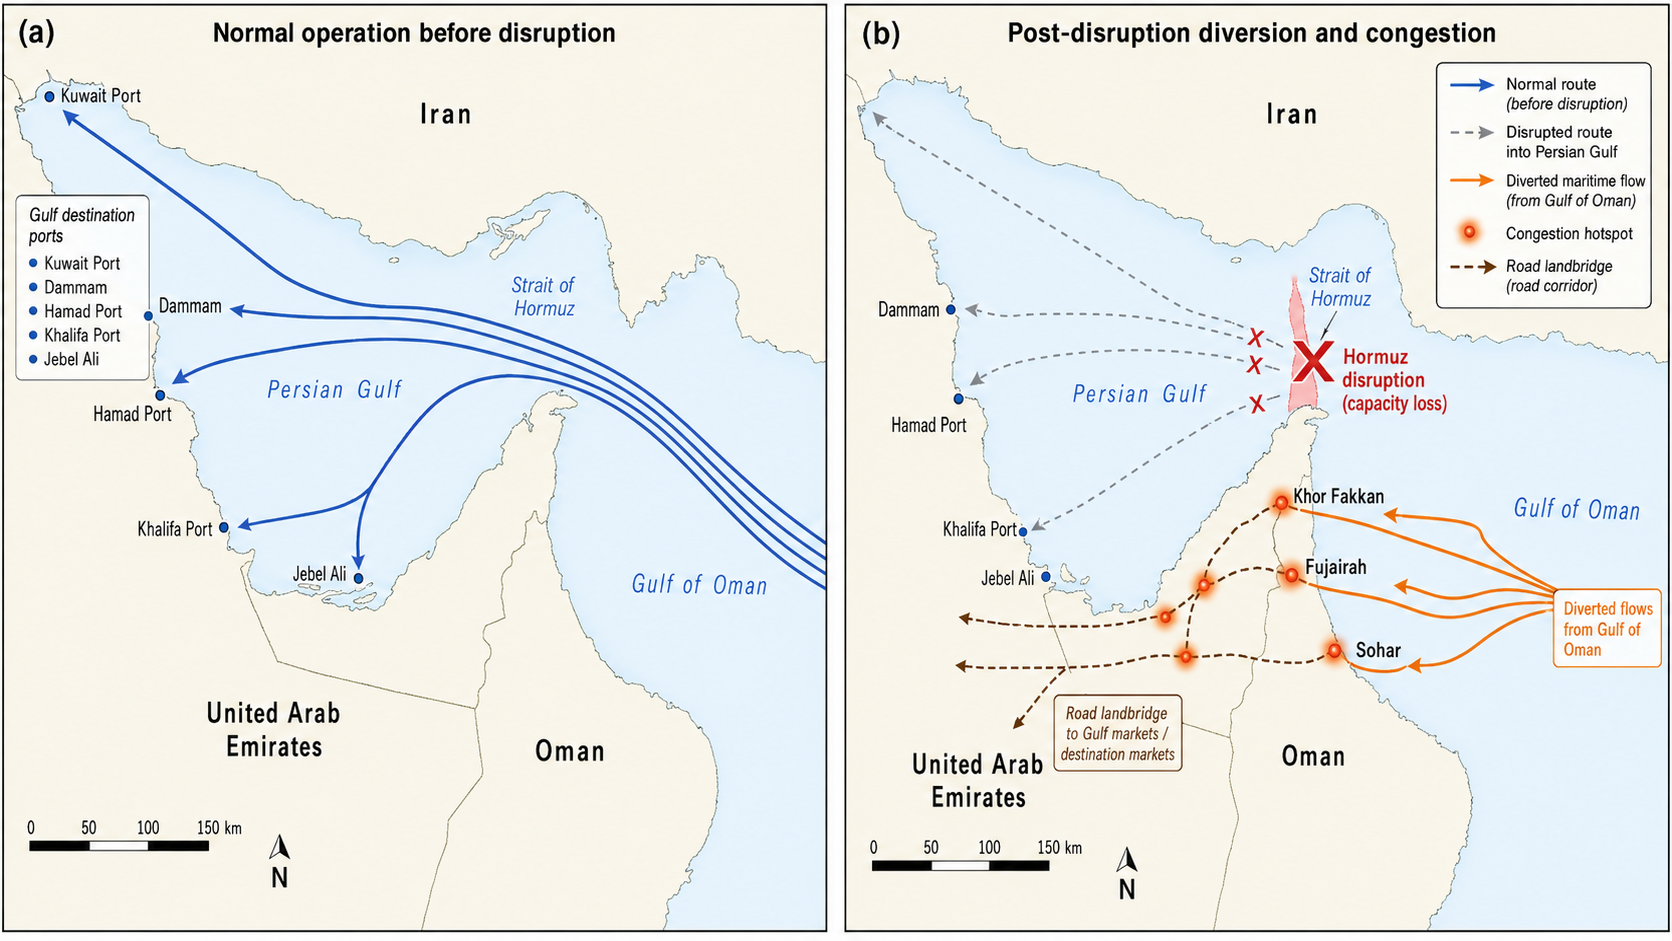
\includegraphics[width=0.75\linewidth]{figures/hormuz comparisation.png}
    \caption{Transportation through the Strait of Hormuz }
    \label{hormuz}
\end{figure}

The resulting diversion does not occur as a single homogeneous flow. Shortly
after the disruption, some vessels and cargoes are already assigned to
particular gateways because of their voyage position, emergency carrier
instructions, terminal arrangements, or short-term contractual commitments.
This component constitutes the committed diversion wave. Its gateway
allocation is treated as exogenous within the relevant operational lead time,
and receiving gateways can respond mainly by mobilising handling and
landside capacity. The remaining flow retains the ability to wait or select
among feasible gateway--landbridge itineraries and forms the adaptive
component, and it has two sources. The portion of the initially blocked cargo whose
gateway is not yet fixed, and newly generated Gulf-bound cargo that arrives
after the disruption and must be routed without recourse to the Hormuz
corridor. Both sources face the same decision and are therefore treated
together. This adaptive component responds to updated and dynamic sailing time, port delay,
handling cost, road congestion, border delay, service reliability, and any
bounded guidance or incentive provided by the regional coordinator. The
committed and adaptive distinction thus reflects whether the gateway assignment
is already locked within the operational lead time, rather than whether the
cargo belongs to the initial blocked wave.

The two components generate different congestion mechanisms. Committed cargo
creates the initial arrival pressure at the receiving gateways. As vessels and
containers accumulate, congestion develops through berth, yard, and
gate/customs operations and subsequently reaches road and border corridors.
Landside congestion reduces the rate at which containers leave the gateway,
which increases yard occupancy and may eventually reduce vessel handling
productivity. Internal port and landside congestion therefore evolve through
a bidirectional physical feedback process. Congestion also affects the later allocation of adaptive cargo. When queues at
one gateway or its connected landbridge increase, the generalised cost of that
itinerary rises. Cargo that remains uncommitted may then select another
gateway, transferring pressure to a previously less congested port and
corridor. Cross-gateway propagation is therefore generated through the
interaction between physical port--hinterland queues and adaptive itinerary
choice. The process can be summarised in Figure \ref{fig:hormuz-structure}.





\begin{figure}
\centering
\definecolor{shockred}{RGB}{192,57,43}
\definecolor{adaptblue}{RGB}{52,152,219}
\definecolor{coordgreen}{RGB}{39,174,96}
\definecolor{queueorange}{RGB}{230,126,34}
\definecolor{softgray}{RGB}{242,244,246}
\begin{tikzpicture}[
    scale=0.82, transform shape,
    >=Latex, font=\small, node distance=10mm and 20mm,
    origin/.style={draw,rounded corners=2pt,align=center,
        minimum height=13mm,text width=28mm,fill=softgray},
    committed/.style={draw=shockred,rounded corners=2pt,align=center,
        minimum height=12mm,text width=28mm,fill=shockred!7},
    adaptive/.style={draw=adaptblue,rounded corners=2pt,align=center,
        minimum height=12mm,text width=28mm,fill=adaptblue!8},
    queue/.style={draw=queueorange!90!black,rounded corners=2pt,align=center,
        minimum height=13mm,text width=32mm,fill=queueorange!8},
    action/.style={draw=coordgreen,rounded corners=2pt,align=center,
        minimum height=13mm,text width=34mm,fill=coordgreen!8},
    commflow/.style={-Latex,very thick,draw=shockred},
    adapflow/.style={-Latex,very thick,dashed,draw=adaptblue},
    phys/.style={-Latex,thick,draw=black!70},
    feedback/.style={-Latex,thick,dashed,draw=adaptblue},
    ctrl/.style={-Latex,thick,draw=coordgreen}
]
% ---- Source splits into committed and adaptive ----
\node[origin] (blocked) {Diverted Gulf-bound\\cargo after disruption};
\node[committed,above right=8mm and 20mm of blocked] (committed)
    {Committed cargo\\gateway fixed};
\node[adaptive,below right=8mm and 20mm of blocked] (adaptive)
    {Adaptive cargo\\gateway selectable};

% ---- Gateway, road, market ----
\node[queue,right=22mm of committed] (gateway)
    {Gateway operations\\Berth $\rightarrow$ Yard $\rightarrow$ Gate};
\node[queue,below=16mm of gateway] (road)
    {Road landbridge\\and border queues};
\node[origin,below right=6mm and 8mm of road,text width=24mm] (market)
    {Gulf inland\\markets};

% ---- Coordinator ----
\node[action,below=16mm of road] (coord)
    {Regional coordinator\\readiness, capacity,\\guidance, incentives};

% ---- Cargo flows ----
\draw[commflow] (blocked) -- (committed);
\draw[adapflow] (blocked) -- (adaptive);
\draw[commflow] (committed) -- (gateway);
\draw[adapflow] (adaptive) -- (gateway.west);

% ---- Physical evacuation ----
\draw[phys] (gateway) -- node[left,font=\scriptsize,pos=0.4]{evacuation} (road);
\draw[phys] (road) -- (market);

% ---- Bidirectional feedback (right side, away from labels) ----
\draw[feedback] (road.east) to[bend right=60]
    node[right,font=\scriptsize,align=left]{landside\\feedback} (gateway.east);

% ---- Adaptive re-selection (label placed low-left to avoid overlap) ----
\draw[feedback] (gateway.south west) to[bend right=15]
    node[below,font=\scriptsize,align=center,pos=0.4]{updated cost}
    (adaptive.north east);

% ---- Coordinator interventions (labels separated) ----
\draw[ctrl] (coord.north west) to[bend left=15]
    node[left,font=\scriptsize,pos=0.6]{capacity} (gateway.south west);
\draw[ctrl] (coord) -- (road);
\draw[ctrl] (coord.west) to[bend left=30]
    node[below,font=\scriptsize,pos=0.5]{incentive} (adaptive.south);

% ---- Legend ----
\node[anchor=west,font=\scriptsize] at ($(coord.south west)+(-0.3,-0.8)$)
    {\textcolor{shockred}{\rule{7mm}{1pt}}\, committed \quad
     \textcolor{adaptblue}{-\,-}\, adaptive / information \quad
     \textcolor{coordgreen}{\rule{7mm}{0.8pt}}\, coordinator action};
\end{tikzpicture}
\caption{Problem structure after a disruption}
\label{fig:hormuz-structure}
\end{figure}


Given this scenario and problem, we focus on predicting and mitigating this port congestion and propagation. Before the
disruption, the coordinator observes a filtered geopolitical risk state and
may undertake reversible readiness actions. Once the disruption is observed,
the coordinator projects diverted cargo and overload risks before physical
congestion fully materialises. It may then activate temporary berth, yard,
gate, truck, and border capacity and modify the information or incentive
component of route costs. The coordinator cannot reverse already committed
gateway assignments and cannot centrally allocate all adaptive cargo.
Independent carriers and forwarders continue to select their own feasible
itineraries.

The research problem is therefore twofold. The first task is to predict where and how severely this disruption will congest the external gateway system, and the second is to decide, within the coordinator's authority, how to mitigate the resulting congestion and its propagation. The model begins from the reduction in Hormuz transit capacity rather than from the military process that produces it. That process is treated as exogenous, and the exact date of the disruption is not assumed to be predictable. Prediction here is therefore understood at two levels. Before any disruption, the coordinator forms a forward-looking assessment of the geopolitical risk state rather than of a precise closure date, using a filtered geopolitical risk index to nowcast the probability that the system is in a crisis regime, and this belief supports low-cost reversible readiness. Once a disruption is observed, the prediction task is to project how much cargo diverts, which gateways and hinterland corridors are most exposed, and when each is likely to cross an operational overload threshold, before physical congestion fully materialises. The mitigation task is to convert this projection into a policy over the coordinator's admissible actions, namely reversible readiness before the disruption and, afterwards, temporary berth, yard, gate, truck, and border capacity together with bounded guidance or incentives on route cost, so as to reduce total congestion, propagation, and cost over the horizon. Because the coordinator can neither reverse committed gateway assignments nor centrally allocate adaptive cargo, the problem is to find such a policy while the diversion and re-selection of cargo remain a decentralised equilibrium response rather than a quantity the coordinator sets directly. Solving it requires a model that captures how the resulting committed and adaptive flows generate, transfer, and potentially amplify congestion across external gateways and their hinterland corridors. 


% Insert the geographical or combined scenario figure here

\subsection{System Setting and Multilayer Network Representation}
\label{subsec:setting}

We consider Gulf-bound container cargo that, following a reduction in Hormuz
transit capacity, can enter the Gulf market through external gateway ports and
road--landbridge/border connections. The unit of flow is 1,000 metric tonnes of
the disclosed AIS-derived activity proxy per decision
period. The period length is chosen to match the finest reliable operational
data, and all service rates, stocks, and costs are converted to that same unit.

There are three actor classes in this problem. First, the external environment generates
the latent geopolitical-risk regime, channel availability, Gulf-bound demand,
market war-risk prices, and unanticipated innovations. These quantities are not
chosen by any actor in the model. Second, a regional coordinator chooses
low-cost readiness before the disruption and, after the disruption, bounded
route guidance and temporary berth, yard, gate, truck, or border capacity. The
coordinator represents an emergency coordination platform rather than a single
port operator. Third, independent carriers and forwarders choose complete
itineraries for cargo that has not yet been committed. Their decentralized
response is a stochastic user equilibrium (SUE), not a centrally assigned flow.





Time is discrete, $t\in\mathcal T=\{0,\ldots,T-1\}$. Let $t_0$ denote the first
period in which the disruption is observed, $t_c$ the first shock-attributable
threshold crossing at a gateway, and $t_p$ the first crossing at another
previously uncongested gateway or a shared landbridge. The general sequence is
\begin{equation}
  t_0 \le t_c \le t_p,
  \label{eq:timeline}
\end{equation}
whenever these stopping times are finite. Equality $t_c=t_0$ represents an
immediate first overload, and $t_p=t_c$ records simultaneous propagation; the
strict ordering in the motivating diagram is the operationally useful warning
window. Before $t_0$, decisions use the filtered
risk-regime belief and are restricted to reversible readiness. From $t_0$
until $t_c$, the disruption state is known, but future duration, arrivals, and
capacity losses remain uncertain; this is the post-shock, pre-congestion
projection window. No formulation below assumes that the exact disruption date
is predictable.

The physical system in period $t$ is
\begin{equation}
  \mathcal G_t=(\mathcal O,\mathcal I,\mathcal D,
  \mathcal E^{M}_t,\mathcal E^{H}_t),
  \label{eq:network}
\end{equation}
where $\mathcal O$ contains ocean origins or route-entry regions,
$\mathcal I$ contains external gateway ports, $\mathcal D$ contains Gulf
markets, $\mathcal E^{M}_t$ contains available maritime connections, and
$\mathcal E^{H}_t$ contains road, border, and landbridge connections.
For compactness, $\mathcal E=\bigcup_t\mathcal E^H_t$ denotes the candidate
landside-corridor set across the study horizon.
The application treats Khor Fakkan, Fujairah, and Sohar as illustrative
gateways, subject to final data availability; all analytical statements use the
generic index $i$ and do not depend on having exactly three ports. A cargo
class $k\in\mathcal K$ identifies an origin--destination market and, when data
permit, a carrier or service class. Its feasible itinerary set is
$\mathcal R_k(t)$. The master physical tag set is
$\overline{\mathcal R}_k=\bigcup_{t\in\mathcal T}\mathcal R_k(t)$: new choices
use only $\mathcal R_k(t)$, whereas an in-transit or queued cohort retains its
tag in $\overline{\mathcal R}_k$ even if that itinerary later closes to new
cargo. An itinerary
\begin{equation}
  r=(o(r),i(r),e(r),d(r))\in\mathcal R_k(t)
  \label{eq:itinerary}
\end{equation}
contains an ocean origin, a gateway $i(r)$, a landbridge/border corridor $e(r)$,
and a final market. Every gateway is internally represented as
berth - yard - gate/customs. Thus, the behavioral
alternative is a complete gateway--landbridge itinerary, not a port in
isolation. Figure~\ref{fig:system-architecture} summarises this multilayer
structure, the internal berth--yard--gate--road resolution of a gateway, the
reverse-capacity feedback, and the adaptive SUE loop.




\begin{figure}
\centering
\definecolor{shockred}{RGB}{192,57,43}
\definecolor{adaptblue}{RGB}{52,152,219}
\definecolor{coordgreen}{RGB}{39,174,96}
\definecolor{queueorange}{RGB}{230,126,34}
\definecolor{fbpurple}{RGB}{142,68,173}
\definecolor{softgray}{RGB}{242,244,246}
\begin{tikzpicture}[
    scale=0.86, transform shape,
    >=Latex, font=\small, node distance=8mm and 14mm,
    net/.style={draw,rounded corners=2pt,align=center,
        minimum height=10mm,text width=22mm,fill=softgray},
    state/.style={draw=queueorange!90!black,rounded corners=2pt,align=center,
        minimum height=10mm,text width=17mm,fill=queueorange!8},
    road/.style={draw=queueorange!90!black,rounded corners=2pt,align=center,
        minimum height=10mm,text width=20mm,fill=queueorange!14},
    adapt/.style={draw=adaptblue,rounded corners=2pt,align=center,
        minimum height=11mm,text width=30mm,fill=adaptblue!8},
    ctrlbox/.style={draw=coordgreen,rounded corners=2pt,align=center,
        minimum height=11mm,text width=32mm,fill=coordgreen!8},
    serv/.style={-Latex,thick,draw=queueorange!80!black},
    fb/.style={-Latex,thick,dashed,draw=fbpurple},
    ctrl/.style={-Latex,thick,draw=coordgreen},
    sue/.style={-Latex,thick,dotted,draw=adaptblue},
    net_e/.style={-Latex,thick,draw=black!65}
]
% ===== Multilayer network layer (top): O -> I -> D =====
\node[net] (O) {Ocean origins\\$\mathcal O$};
\node[net,right=20mm of O] (I) {Gateways\\$\mathcal I=\{i\}$};
\node[net,right=20mm of I] (D) {Gulf markets\\$\mathcal D$};
\draw[net_e] (O) -- node[above,font=\scriptsize]{$\mathcal E^{M}_t$} (I);
\draw[net_e] (I) -- node[above,font=\scriptsize]{$\mathcal E^{H}_t$} (D);
\node[font=\scriptsize,above=1mm of I] {itinerary $r=(o,i,e,d)$};

% ===== Expanded gateway i: berth -> yard -> gate -> road (bottom) =====
\node[state,below=16mm of O] (B) {Berth\\$B_{it}$};
\node[state,right=of B] (Y) {Yard\\$Y_{it}$};
\node[state,right=of Y] (G) {Gate\\$G_{it}$};
\node[road,right=of G] (M) {Road/border\\$M_{et}$};

% arrivals into berth
\node[font=\scriptsize,left=7mm of B] (Ain) {$A_{it}$};
\draw[serv] (Ain) -- (B);
% service flows
\draw[serv] (B) -- node[above,font=\scriptsize]{$H_{it}$} (Y);
\draw[serv] (Y) -- node[above,font=\scriptsize]{$D_{it}$} (G);
\draw[serv] (G) -- node[above,font=\scriptsize]{$R_{it}$} (M);
\draw[serv] (M) -- node[above,font=\scriptsize]{$K_{et}$} ++(2.4,0)
    node[right,font=\scriptsize] {to $\mathcal D$};
% effective-capacity labels under each stage
\node[font=\scriptsize,below=1mm of B] {$\mu^{B,\mathrm{eff}}_{it}$};
\node[font=\scriptsize,below=1mm of Y] {$\mu^{Y,\mathrm{eff}}_{it}$};
\node[font=\scriptsize,below=1mm of G] {$\mu^{G,\mathrm{eff}}_{it}$};
\node[font=\scriptsize,below=1mm of M] {$\kappa^{\mathrm{eff}}_{et}$};

% ===== Reverse feedback multipliers (below the chain) =====
% psi^Y: yard occupancy reduces berth capacity
\draw[fb] (Y.south) to[bend left=40]
    node[below,font=\scriptsize]{$\psi^Y_i(Y_{it}/\bar Y_i)$} (B.south);
% psi^M: road congestion reduces gate capacity
\draw[fb] (M.south) to[bend left=40]
    node[below,font=\scriptsize]{$\psi^M_i(\sum_e\omega_{iet}M_{et}/\bar M_e)$} (G.south);

% ===== SUE fixed-point loop (adaptive re-selection) =====
\node[adapt,below=30mm of Y] (sue)
    {Route--waiting SUE\\$(x_t^{*},w_t^{*})=\mathcal L_t(x_t^{*},w_t^{*})$};
\node[adapt,left=11mm of sue,text width=21mm] (wait)
    {External waiting\\$W_{t+1}$};
\node[net,left=8mm of wait,text width=17mm] (exit)
    {System exit\\$e_t$};
% cost out of the gateway states into SUE
\draw[sue] (G.south) to[bend right=18]
    node[right,font=\scriptsize,align=left,pos=0.55]
    {generalised cost\\$C_{krt}(\widehat W^{B},\widehat W^{Y},\widehat W^{G},\widehat W^{M})$}
    (sue.north east);
% SUE feeds arrivals back to berth
\draw[sue] (sue.north west) to[bend left=18]
    node[left,font=\scriptsize,pos=0.5]{$A_{it}=A^{\mathrm{base}}+\sum(q^C+x^{*})$}
    (B.south west);
\draw[sue] (sue) -- node[above,font=\scriptsize]{$w_t^{*}$} (wait);
\draw[sue] (wait) to[bend left=25]
    node[below,font=\scriptsize]{$\rho_tW_t$} (sue.south west);
\draw[net_e] (exit) -- (wait);

% ===== Coordinator controls (green) =====
\node[ctrlbox,below=10mm of sue] (coord)
    {Coordinator action $a_t$\\readiness, release, capacity, guidance};
\draw[ctrl] (coord.north west) to[bend left=12]
    node[left,font=\scriptsize,pos=0.6]{$v$ (capacity)} (B.south west);
\draw[ctrl] (coord.north) -- node[right,font=\scriptsize]{$v$} (M.south);
\draw[ctrl] (coord.east) to[bend right=25]
    node[right,font=\scriptsize,pos=0.5]{$u$ (cost)} (sue.south east);

% ===== Legend =====
\node[anchor=west,font=\scriptsize] at ($(coord.south west)+(-0.2,-0.8)$)
    {\textcolor{queueorange!80!black}{\rule{7mm}{1pt}}\, service flow \quad
     \textcolor{fbpurple}{-\,-}\, feedback multiplier \quad
     \textcolor{adaptblue}{$\cdots$}\, SUE cost--flow loop \quad
     \textcolor{coordgreen}{\rule{7mm}{0.8pt}}\, control};
\end{tikzpicture}
\caption{Network model structure}
\label{fig:system-architecture}
\end{figure}



Table~\ref{tab:notation} collects the symbols used in the main text. Route-tagged
port states preserve physical flow conservation, while uppercase states are the
aggregates observed by the controller and used in congestion costs. This
construction avoids equating an itinerary selected at sea with a truck that
instantaneously enters a landbridge.

\begin{table}
\centering
\caption{Core notation}
\label{tab:notation}
\small
\begin{tabularx}{\textwidth}{@{}p{0.22\textwidth}X@{}}
\toprule
Symbol & Definition \\
\midrule
$\mathcal I,\mathcal E,\mathcal K,\mathcal R_k(t),\overline{\mathcal R}_k$ &
Gateway ports, corridors, cargo classes, current choice set, and master
physical tag set. \\
$a_t^H\in[0,1]$ & Fraction of baseline Gulf-bound demand serviceable through
Hormuz after capacity loss and any priority allocation. \\
$q^{G}_{kt},q^{B}_{kt}$ & Baseline Gulf-bound demand and the portion blocked by
the disruption. \\
$\chi_{kt}$ & Share of blocked demand whose itinerary is already committed. \\
$q^{C}_{krt},x_{krt}$ & Committed and adaptive route flows; $x_{krt}$ is
endogenous. \\
$b_{krt},y_{krt},g_{krt}$ & Route-tagged berth workload, yard stock, and
gate/customs queue at gateway $i(r)$. \\
$B_{it},Y_{it},G_{it},M_{et}$ & Aggregate berth, yard, gate, and landbridge
states. \\
$h_{krt},d_{krt},r_{krt},K_{et}$ & Berth release, yard release, gate release to
the landbridge, and landbridge discharge. \\
$u_{rt}$ & Bounded route cost adjustment; positive is a penalty and negative a
subsidy. \\
$v^B_{it},v^Y_{it},v^G_{it},v^M_{et}$ & Temporary capacity additions at berth,
yard, gate, and landbridge. \\
$y_t^R,r_t^R,\mathfrak b_t$ & Readiness purchases, active readiness stock, and
remaining coordinator budget. \\
$\bar B_i,\bar Y_i,\bar G_i,\bar M_e$ & Operational congestion thresholds. \\
$\theta_k$ & Sensitivity of class $k$ to generalized itinerary cost. \\
\bottomrule
\end{tabularx}
\end{table}

\subsection{Flow Construction and Feasibility Conditions}
\label{subsec:flow}

This subsection defines the behavioral mass, its physical loading, and the
conditions that keep every modeled cargo unit traceable. All demand, inventory,
service, capacity, and threshold quantities use a common conservation unit
$U_Q$. When the empirical input is an AIS activity proxy that cannot be
reliably converted into tonnes or container units, $U_Q$ is interpreted as a
standardized cargo exposure unit. The application is then a public data
calibrated simulation rather than an observed physical tonnage account.
Baseline gateway arrivals $A^{\mathrm{base}}$ are exogenous conditional
scenarios. This assumption does not imply that normal traffic is behaviorally
invariant outside the emergency model.

Let $q^G_{kt}$ denote the Gulf bound demand of class $k$ that would use the
Hormuz corridor in period $t$. When priority allocation is represented, the
serviceable share is class specific and the newly blocked mass is
\begin{equation}
 q^B_{kt}=(1-a^H_{kt})q^G_{kt}.
 \label{eq:blocked-flow}
\end{equation}
A common serviceable share $a^H_t$ is the restricted case used when class
specific serviceability cannot be identified. The modeled blocked cohort has
only two initial components
\begin{equation}
 q^C_{kt}=\chi_{kt}q^B_{kt},\qquad
 q^D_{kt}=(1-\chi_{kt})q^B_{kt}.
 \label{eq:commitment-split}
\end{equation}
The committed component $q^C_{kt}$ has a complete itinerary fixed at its
commitment time. The decision eligible component $q^D_{kt}$ can choose a route,
waiting, or exit. Cancellation or movement outside the study region that
occurs before $q^B_{kt}$ is constructed is excluded and reported separately.
It is not a behavioral exit in this model and does not enter a policy
improvement measure.

Committed itinerary shares satisfy
\begin{equation}
 q^C_{krt}=\delta^C_{krt}q^C_{kt},\qquad
 \sum_{r\in\mathcal R_k^{\mathrm{com}}(t)}
 \delta^C_{krt}=1,\qquad \delta^C_{krt}\ge0.
 \label{eq:committed-route-share}
\end{equation}
The set $\mathcal R_k^{\mathrm{com}}(t)$ records the itineraries that could be
contracted when the cohort became committed. Once assigned, tag $r$ remains
with that cargo. A later change in the choice set for new cargo neither
renormalizes the shares nor reallocates an existing tagged cohort. If a tagged
link becomes temporarily unavailable, its physical service is zero and the
cargo remains in its tagged pipeline or queue. The cohort parameter
$\chi_{kt}$ applies only to new blocked cargo. It is not a decay rate for
existing committed inventory.

External waiting is represented by age vintages. Let
\begin{equation}
 W_{kt}=\sum_{j=0}^{\bar J}W_{ktj},\qquad
 W_{ktj}\ge0,
 \label{eq:waiting-vintages}
\end{equation}
where $W_{ktj}$ is the beginning of period mass that has already waited $j$
periods outside the gateway system. The coordinator selects a class specific
total release rate
\begin{equation}
 0\le\rho_{kt}\le1,\qquad
 R^W_{kt}=\rho_{kt}W_{kt}.
 \label{eq:waiting-release}
\end{equation}
A deterministic oldest first operator allocates this total across vintages
\begin{equation}
 \left(R^W_{kt0},\ldots,R^W_{kt\bar J}\right)
 =
 \operatorname{OF}\!\left(
 R^W_{kt};W_{kt0},\ldots,W_{kt\bar J}
 \right),
 \quad
 0\le R^W_{ktj}\le W_{ktj},\quad
 \sum_jR^W_{ktj}=R^W_{kt}.
 \label{eq:oldest-first}
\end{equation}
The policy controls $\rho_{kt}$ but does not choose vintage specific release.
The operator exhausts the oldest nonempty vintage before releasing a younger
one.

The source index $h\in\{N,0,\ldots,\bar J\}$ distinguishes a new decision
eligible cohort from a released waiting vintage. Its decision mass is
\begin{equation}
 d_{kNt}=q^D_{kt},\qquad d_{kjt}=R^W_{ktj}.
 \label{eq:decision-masses}
\end{equation}
For each source, $x_{krht}$ denotes route dispatch, $w_{kht}$ denotes renewed
waiting, and $e^S_{kht}$ denotes a direct SUE exit. These outcomes satisfy
\begin{equation}
 \sum_{r\in\mathcal R_k(t)}x_{krht}
 +w_{kht}+e^S_{kht}=d_{kht}.
 \label{eq:source-conservation}
\end{equation}

Waiting duration creates a second endogenous exit channel. Let the exogenous
hazard be nondecreasing and terminal
\begin{equation}
 0\le\vartheta_k(0)\le\cdots\le
 \vartheta_k(\bar J)=1.
 \label{eq:waiting-hazard}
\end{equation}
For every released old vintage, renewed waiting retains its age
\begin{subequations}\label{eq:waiting-transition}
\begin{align}
 \widetilde W_{ktj}
 &=W_{ktj}-R^W_{ktj}+w_{kjt},\\
 o^W_{ktj}
 &=\vartheta_k(j)\widetilde W_{ktj},\\
 W_{k,t+1,j+1}
 &=(1-\vartheta_k(j))\widetilde W_{ktj},
 &&j=0,\ldots,\bar J-1,\\
 W_{k,t+1,0}&=w_{kNt}.
\end{align}
\end{subequations}
The maximum vintage does not continue because its hazard equals one. The
hazard is a model parameter, while realized attrition $o^W_{ktj}$ changes with
the waiting stock, release, and equilibrium waiting choice. Total modeled exit
is
\begin{equation}
 e^{\mathrm{end}}_{kt}
 =\sum_h e^S_{kht}+\sum_j o^W_{ktj}.
 \label{eq:endogenous-exit}
\end{equation}
Direct SUE exit and duration attrition occur at different decision points.
They are therefore mutually exclusive for each cargo unit. Combining the
source simplex and vintage transition gives the period mass identity
\begin{equation}
 q^D_{kt}+\sum_jW_{ktj}
 =
 \sum_h\sum_r x_{krht}
 +\sum_he^S_{kht}
 +\sum_jo^W_{ktj}
 +\sum_jW_{k,t+1,j}.
 \label{eq:adaptive-conservation}
\end{equation}
Finite $\bar J$, terminal attrition, and bounded new demand imply a finite
bound on external waiting. They do not imply that simulated waiting must
converge to a plateau.

The timing within each period is fixed. The beginning state contains
information completed by period $t-1$, mature readiness, active direct
capacity, all waiting vintages, all route tagged queues, the maritime pipeline,
and the history required for corridor weights. Newly released monthly
information and observed event status are incorporated before the action. The
coordinator then chooses
\begin{equation}
 a_t=(y^R_t,y^V_t,v^R_t,\rho_t,\lambda_t).
 \label{eq:formal-action}
\end{equation}
The oldest first operator constructs vintage releases. Carriers next solve the
source specific route, waiting, and exit SUE using waiting costs that already
internalize the period attrition hazard. Route dispatch enters the maritime
pipeline. Zero lag mass enters the current berth arrival at the declared
external arrival point. Current service then uses capacity already available
in period $t$. Attrition is applied to unreleased and renewed old waiting
vintages before all states move to period $t+1$. Current realizations and the
ex post crossing times $t_c$ and $t_p$ cannot affect the action already taken.

Aggregating route choices across sources gives
\begin{equation}
 x_{krt}=\sum_hx_{krht}.
 \label{eq:route-dispatch}
\end{equation}
Committed and endogenous dispatch use the same maritime lag kernel
\begin{equation}
 A_{krt}=A^{\mathrm{base}}_{krt}+P^{M,0}_{krt}
 +\sum_{\substack{0\le\tau\le\bar\tau_r\\t-\tau\ge0}}
 \ell^M_{kr,\tau\mid t-\tau}
 \left(q^C_{kr,t-\tau}+x_{kr,t-\tau}\right).
 \label{eq:route-arrival}
\end{equation}
The kernel is normalized within each dispatch cohort. Undelivered mass is
stored in $\mathbf P^M_t$ with remaining lag, class, route tag, and provenance
$c\in\{C,A\}$. This provenance identifies future committed arrivals in the
physical boundary below. If a route closes to new choices, already dispatched
mass remains in the master tag set $\overline{\mathcal R}_k$. When a tagged
physical link is unavailable, the affected pipeline mass remains in its
upstream holding position until service resumes.

Cargo keeps its class and itinerary tag through berth, yard, gate, and
landbridge operations. For each $k$, $r\in\overline{\mathcal R}_k$, and $t$,
\begin{subequations}\label{eq:tagged-conservation}
\begin{align}
 b_{kr,t+1}&=b_{krt}+A_{krt}-s^B_{krt},
 \label{eq:berth-balance}\\
 y_{kr,t+1}&=y_{krt}+s^B_{krt}-s^Y_{krt},
 \label{eq:yard-balance}\\
 g_{kr,t+1}&=g_{krt}+s^Y_{krt}-s^G_{krt}.
 \label{eq:gate-balance}
\end{align}
\end{subequations}
The route tagged landbridge balance is
\begin{equation}
 m_{kr,t+1}=m_{krt}+s^G_{krt}-s^M_{krt}.
 \label{eq:landbridge-balance}
\end{equation}
The aggregate states are
\begin{equation}
 B_{it}=\sum_{k,r:i(r)=i}b_{krt},\qquad
 M_{et}=\sum_{k,r:e(r)=e}m_{krt},
 \label{eq:aggregate-tagged-states}
\end{equation}
with analogous definitions for $Y_{it}$ and $G_{it}$. Delivered cargo is the
cumulative landbridge discharge $\sum_{t,k,r}s^M_{krt}$. Gate release is not
delivery.

External arrival is available to berth service in its arrival period. An
internal stage release enters the downstream inventory in the next period and
cannot receive a second internal service in the current period. Aggregate
service is
\begin{subequations}\label{eq:work-conserving}
\begin{align}
 \mathcal S^B_{it}
 &=\min\{B_{it}+A_{it},\mu^{B,\mathrm{eff}}_{it}\},\\
 \mathcal S^Y_{it}
 &=\min\{Y_{it},\mu^{Y,\mathrm{eff}}_{it}\},\\
 \mathcal S^G_{it}
 &=\min\{G_{it},\mu^{G,\mathrm{eff}}_{it}\},\\
 \mathcal S^M_{et}
 &=\min\{M_{et},\kappa^{\mathrm{eff}}_{et}\}.
\end{align}
\end{subequations}
Each aggregate amount is allocated in proportion to the corresponding
preservice tagged workload. For example
\begin{equation}
 s^B_{krt}=
 \frac{b_{krt}+A_{krt}}{B_{it}+A_{it}}\mathcal S^B_{it},
 \qquad
 s^M_{krt}=\frac{m_{krt}}{M_{et}}\mathcal S^M_{et},
 \label{eq:proportional-service}
\end{equation}
where a ratio is zero when its denominator is zero. The same rule defines
$s^Y$ and $s^G$. This rule is proportional sharing rather than a first in first
out discipline. Temporary yard capacity changes the yard processing rate only.
It does not also change the yard storage threshold. Maritime and internal
travel lags remain physical inputs, while anticipated waiting responds to
projected queues.

The topology permits genuine shared corridor coupling when
\begin{equation}
 \exists e^\star\in\mathcal E
 \quad\text{such that}\quad
 \left|\{i:\exists r,\ i(r)=i,\ e(r)=e^\star\}\right|\ge2.
 \label{eq:shared-corridor}
\end{equation}
Several gateways can then load the same tagged landbridge inventory and compete
for the same corridor capacity. No additional border post queue is required.
If the empirical itinerary set contains no shared corridor, the application
can claim propagation through route reselection but not through a shared
physical corridor.

\begin{proposition}[Adaptive choice shaping boundary]
\label{prop:controllability}
Fix the state, new demand, and release vector. Let
$\mathcal C_k(t)=\mathcal R_k(t)\cup\{\mathsf W,\mathsf E\}$.
For any two feasible choice patterns $z$ and $z'$ with the same source decision
masses $d_{kht}$,
\begin{equation}
 \frac12\sum_{k,h}\sum_{\ell\in\mathcal C_k(t)}
 |z'_{kh\ell t}-z_{kh\ell t}|
 \le\sum_{k,h}d_{kht}.
 \label{eq:shapeable-bound}
\end{equation}
\end{proposition}
This bound includes route choice, renewed waiting, and direct SUE exit. It
excludes unreleased waiting, duration attrition, and committed cargo. It is a
one period bound on decision eligible mass. It is not a quantitative effect of
disclosure and it is not a cumulative dynamic sensitivity result. Policies
with different release vectors have different source masses and are outside
this fixed release comparison.

The committed physical boundary uses a time expanded relaxed network. The
network begins from the complete observed queue state and retains all legacy
workload. Future base and adaptive arrivals are removed, while committed
arrivals already present in the maritime pipeline are retained. Feedback
multipliers take their most favorable values. Service uses the componentwise
capacity envelope over feasible actions. The shared budget is relaxed and
nonwork conserving service is permitted. For a single gateway, every reachable
shared corridor can be allocated optimistically to that gateway. The resulting
maximum absorbable committed arrival is
\begin{equation}
 \mathcal C^{\mathrm{abs}}_{it}(H)=
 \max_{(\widetilde A^C,\mathbf f,\mathbf S)
 \in\mathcal F^{\mathrm{TE}}_{it}(H)}
 \sum_{\tau=0}^{H-1}
 \sum_{k,r:i(r)=i}\widetilde A^C_{kr,t+\tau}.
 \label{eq:absorption-capacity}
\end{equation}
The quantity for the actual committed pipeline is
\begin{equation}
 \mathcal Q^C_{it}(H)=
 \sum_{\tau=0}^{H-1}
 \sum_{k,r:i(r)=i}A^C_{kr,t+\tau}.
 \label{eq:committed-arrivals-window}
\end{equation}

\begin{proposition}[Unavoidable congestion boundary]
\label{prop:absorption}
If
\begin{equation}
 \mathcal Q^C_{it}(H)>
 \mathcal C^{\mathrm{abs}}_{it}(H),
 \label{eq:unavoidable-condition}
\end{equation}
then every feasible policy causes at least one associated berth, yard, gate,
or reachable corridor state to exceed its absolute operational threshold in
the window.
\end{proposition}
The first horizon $H^\star$ that satisfies
\cref{eq:unavoidable-condition} is an upper bound on the latest guaranteed
crossing time. The smallest capacity increment that makes this optimistic
certificate disappear is only a lower bound on necessary capacity. It is not a
sufficient intervention. Gateway specific bounds cannot be added because they
may each receive the same shared corridor capacity in their separate relaxed
problems. This proposition uses absolute thresholds. The ex post times $t_c$
and $t_p$ use a matched no disruption counterfactual and serve a different
attribution purpose. Proofs of both propositions are in
\Cref{app:proofs}.

\subsection{Equilibrium Driven Port and Hinterland Congestion Dynamics}
\label{subsec:dynamics}

The physical loading is endogenous because carriers compare route, waiting,
and exit outcomes for every new or released source. The within period SUE is
followed by the interperiod transition in \cref{subsec:flow}. This construction
matches the available data frequency and does not claim a continuous time
dynamic user equilibrium.

For any candidate choice vector $z_t$, anticipated waiting uses a deterministic
continuous queue projection
\begin{equation}
 \widehat W^q_{j_q(r),rt}(z_t;s_t,a_t)=
 \frac{
 \widehat Q^q_{j_q(r),t+\tau_r^q}
 +\widehat I^q_{j_q(r),t+\tau_r^q}
 }{
 \widehat\mu^{q,\mathrm{eff}}_{j_q(r),t+\tau_r^q}
 +\epsilon
 },
 \qquad q\in\{B,Y,G,M\}.
 \label{eq:anticipated-wait}
\end{equation}
The continuation rule and representative exogenous path remain fixed during
one SUE solution. Stochastic scenario sampling occurs in the outer MPC or
policy rollout. It is not recursively resampled inside every SUE iteration.
A cache may store only quantities independent of the candidate vector.
Candidate route and waiting flows must retain their marginal effect on
projected workload.

Information intervention is a verifiable disclosure decision. Let
$\widetilde{\mathcal W}_{krt}(z_t)$ be the carrier private prior for anticipated
door to door waiting. Let
$\widetilde{\mathcal W}^{\mathrm{ref}}_{krt}$ be a reference forecast frozen
before the action. Let
$\widehat{\mathcal W}^{\mathrm{pub}}_{krt}(s_t,a_t^{-I})$ be the verifiable
queue based signal available before choice. The disclosure intensity
$\lambda_{krt}\in[0,1]$ gives perceived waiting
\begin{equation}
 \mathcal W^{\mathrm{perc}}_{krt}(z_t)=
 (1-\lambda_{krt})\widetilde{\mathcal W}_{krt}(z_t)
 +\lambda_{krt}
 \widehat{\mathcal W}^{\mathrm{pub}}_{krt}(s_t,a_t^{-I}).
 \label{eq:disclosed-wait}
\end{equation}
The coordinator selects the weight between the prior and signal but cannot
select the sign of their difference. The public signal can reflect capacity
and release decisions already announced in $a_t^{-I}$. It is constructed with
a predetermined reference loading rule and cannot be inferred backward from
the equilibrium that the signal induces.

Credibility is defined in time units
\begin{equation}
 \bar\delta^W_{krt}=\gamma_I\sigma^W_{krt},\qquad
 0\le\gamma_I\le1,\qquad
 \left|
 \widehat{\mathcal W}^{\mathrm{pub}}_{krt}
 -\widetilde{\mathcal W}^{\mathrm{ref}}_{krt}
 \right|\le\bar\delta^W_{krt}.
 \label{eq:disclosure-credibility}
\end{equation}
The error scale $\sigma^W_{krt}$ and signal construction are fixed before
solving the current action and SUE. Multistart equilibrium dispersion is not a
substitute for forecast error. An ex post credibility audit compares realized
time error with $\bar\delta^W$. The monetary equivalent is
$\nu_k\bar\delta^W$. Information acquisition, verification, and publication
cost $c^I(\lambda_t)$ enters the budget and formal objective.

The route generalized cost is
\begin{equation}
 C^R_{krt}(z_t;s_t,a_t)=
 c^{\mathrm{private,res}}_{kr}
 +c^{\mathrm{mkt}}_{krt}
 +\nu_k\mathcal W^{\mathrm{perc}}_{krt}(z_t).
 \label{eq:generalized-cost}
\end{equation}
Private resource use, market risk perception, and perceived waiting govern
carrier behavior. They are not copied without adjustment into the coordinator
objective.

The candidate end of period waiting inventory is
\begin{equation}
 \widehat W^{\mathrm{out}}_{k,t+1}(z_t)=
 w_{kNt}+
 \sum_{j=0}^{\bar J}
 (1-\vartheta_k(j))
 \left(W_{ktj}-R^W_{ktj}+w_{kjt}\right).
 \label{eq:projected-waiting}
\end{equation}
For source $h$, define the current waiting resource and inventory cost
\begin{equation}
 \bar C^W_{kht}(z_t)=
 c^{W,0}_k+c^{W,\mathrm{age}}_k(\operatorname{age}(h))
 +c^{W,I}_k
 \frac{\widehat W^{\mathrm{out}}_{k,t+1}(z_t)}
 {\bar W_k+\epsilon}
 +c^{W,R}_k\widehat p^{\mathrm{reclose}}_t,
 \label{eq:waiting-resource-cost}
\end{equation}
where $c^{W,\mathrm{age}}_k$ is nondecreasing. The Bellman consistent waiting
cost is
\begin{equation}
 C^W_{kht}(z_t)=
 \bar C^W_{kht}(z_t)
 +p^{\mathrm{attr}}_{kh}C^{E,A}_{kht}
 +(1-p^{\mathrm{attr}}_{kh})
 \widehat V^W_{k,\operatorname{next}(h),t+1}.
 \label{eq:waiting-cost}
\end{equation}
For a new cohort,
\begin{equation}
 \operatorname{age}(N)=0,\qquad
 \operatorname{next}(N)=0,\qquad
 p^{\mathrm{attr}}_{kN}=0.
 \label{eq:new-source-age}
\end{equation}
For a released vintage $h=j$ that chooses to wait again,
\begin{equation}
 \operatorname{age}(j)=j+1,\qquad
 \operatorname{next}(j)=j+1,\qquad
 p^{\mathrm{attr}}_{kj}=\vartheta_k(j).
 \label{eq:old-source-age}
\end{equation}
The convention
$\widehat V^W_{k,\bar J+1,t+1}=0$ removes continuation after the terminal
vintage. The attrition consequence uses
\begin{equation}
 C^{E,A}_{kjt}=C^E_{kjt}+c^{E,\mathrm{late}}_{kj},
 \qquad c^{E,\mathrm{late}}_{kj}\ge0.
 \label{eq:attrition-consequence}
\end{equation}
If no additional late failure consequence is identified,
$c^{E,\mathrm{late}}_{kj}=0$. Direct SUE exit has private cost
\begin{equation}
 C^E_{kht}=
 c^{E,\mathrm{lost}}_{kht}
 +c^{E,\mathrm{contract}}_{kht}
 +c^{E,\mathrm{replacement}}_{kht}.
 \label{eq:exit-cost}
\end{equation}
The direct and duration exit channels therefore share the same underlying
economic consequences. The operational failure cost in the coordinator
objective is conceptually distinct.

Let
\begin{equation}
 \mathcal C_k(t)=
 \mathcal R_k(t)\cup\{\mathsf W,\mathsf E\}.
 \label{eq:choice-set}
\end{equation}
For route label $r$, waiting label $\mathsf W$, and exit label $\mathsf E$, use
$C_{khr t}=C^R_{krt}$,
$C_{kh\mathsf Wt}=C^W_{kht}$, and
$C_{kh\mathsf Et}=C^E_{kht}$. The Logit loading is
\begin{equation}
 [\mathcal L_t(z_t;s_t,a_t)]_{kh\ell}=
 d_{kht}
 \frac{\exp\{-\theta_k C_{kh\ell t}(z_t;s_t,a_t)\}}
 {\sum_{\ell'\in\mathcal C_k(t)}
 \exp\{-\theta_k C_{kh\ell't}(z_t;s_t,a_t)\}}.
 \label{eq:logit-loading}
\end{equation}
A zero mass source is assigned zero flow without evaluating the softmax. The
equilibrium set is
\begin{equation}
 z_t^\star\in
 \operatorname{Fix}\mathcal L_t(\cdot;s_t,a_t).
 \label{eq:sue-fixed-point}
\end{equation}
Physical dispatch is
$x^\star_{krt}=\sum_hz^\star_{khrt}$. Waiting and direct exit remain indexed by
source for the vintage transition.

A deterministic selector makes the physical transition single valued. It
compares normalized shares on the master choice set, assigns zero share to an
unavailable route, and excludes zero mass sources from the distance. It first
selects the residual qualified fixed point nearest the preceding normalized
share vector and then applies a fixed lexicographic tie rule
\begin{equation}
 z_t^\star=
 \operatorname{Sel}_t\!\left(
 \operatorname{Fix}\mathcal L_t(\cdot;s_t,a_t)
 \right).
 \label{eq:equilibrium-selector}
\end{equation}
This selector does not establish global continuity. Multinomial Logit is the
main behavioral model. Its independence of irrelevant alternatives property
is a limitation and a potential robustness extension rather than an additional
main model.

\begin{proposition}[Existence of the within period SUE]
\label{prop:sue-existence}
Suppose all source vintages and choice sets are finite. Suppose decision masses
are finite and the queue projection, disclosure map, waiting cost, and exit
cost are continuous in $z_t$. Then the fixed point set in
\cref{eq:sue-fixed-point} is nonempty.
\end{proposition}
The result follows from Brouwer because the product of source specific
simplices is nonempty, compact, and convex, and the Logit loading continuously
maps it into itself. Existence does not imply uniqueness or convergence of a
particular numerical method. A contraction claim requires a verified
Lipschitz constant below one in a declared norm. The proof is in
\Cref{app:proofs}.

Active direct capacity and exercised readiness capacity enter the same physical
service equations. Effective capacities are
\begin{subequations}\label{eq:effective-capacities}
\begin{align}
 \mu^{B,\mathrm{eff}}_{it}
 &=
 \left(
 \bar\mu_i^B+\widetilde n^{V,B}_{it}
 +E^{R,B}v^{R,B}_{it}
 \right)
 \psi_i^Y(Y_{it}/\bar Y_i),\\
 \mu^{Y,\mathrm{eff}}_{it}
 &=
 \bar\mu_i^Y+\widetilde n^{V,Y}_{it}
 +E^{R,Y}v^{R,Y}_{it},\\
 \mu^{G,\mathrm{eff}}_{it}
 &=
 \left(
 \bar\mu_i^G+\widetilde n^{V,G}_{it}
 +E^{R,G}v^{R,G}_{it}
 \right)
 \psi_i^M\!\left(
 \sum_{e\in\mathcal E_i}
 \omega_{ie,t}\frac{M_{et}}{\bar M_e}
 \right),\\
 \kappa^{\mathrm{eff}}_{et}
 &=
 \bar\kappa_e+\widetilde n^{V,M}_{et}
 +E^{R,M}v^{R,M}_{et}.
\end{align}
\end{subequations}
The positive bounded functions $\psi^Y$ and $\psi^M$ are nonincreasing. The
main model supports two physical feedback channels
\begin{equation}
 \begin{gathered}
 Y_i\uparrow\ \Longrightarrow\
 \mu_i^{B,\mathrm{eff}}\downarrow\
 \Longrightarrow B_i\uparrow,\\
 M_e\uparrow\ \Longrightarrow\
 \mu_i^{G,\mathrm{eff}}\downarrow\
 \Longrightarrow G_i\uparrow.
 \end{gathered}
 \label{eq:feedback-chain}
\end{equation}
No equation makes gate occupancy reduce yard service. The model therefore does
not claim that additional reverse link.

For gateway $i$, tagged gate release to corridor $e$ is
\begin{equation}
 F_{ie,t}=
 \sum_{k,r:i(r)=i,e(r)=e}s^G_{krt}.
 \label{eq:corridor-release}
\end{equation}
Corridor weights use a strictly lagged window
\begin{equation}
 \omega_{ie,t}=
 \frac{\sum_{\ell=1}^{n_\omega}F_{ie,t-\ell}}
 {\sum_{e'\in\mathcal E_i}
  \sum_{\ell=1}^{n_\omega}F_{ie',t-\ell}}.
 \label{eq:lagged-corridor-weight}
\end{equation}
When the denominator is zero, a commitment time conditional share is used.
The history
$\mathcal H^\omega_t=
\{F_{ie,t-1},\ldots,F_{ie,t-n_\omega}\}$
is part of the Markov state. When several gateways share $e^\star$, its common
inventory enters every associated gate multiplier and creates the physical
shared corridor channel.

Threshold crossing is an ex post trajectory statistic. Define
\begin{subequations}\label{eq:congestion-indicators}
\begin{align}
 z^P_{it}&=\ind\!\left\{
 \max(B_{it}/\bar B_i,Y_{it}/\bar Y_i,G_{it}/\bar G_i)\ge1
 \right\},\\
 z^M_{et}&=\ind\{M_{et}/\bar M_e\ge1\}.
\end{align}
\end{subequations}
Matched no disruption indicators use the same baseline demand and innovations.
The first shock attributable gateway crossing is $t_c$. The first crossing at
another gateway or a shared corridor is $t_p$. Formally
\begin{subequations}\label{eq:cascade-times}
\begin{align}
 t_c&=\min\{t\ge t_0:\mathcal N^P_t\ne\varnothing\},\\
 t_p&=\min\left\{t\ge t_c:
 (\mathcal N^P_t\setminus\{i_c\})\cup
 \mathcal N^M_t\ne\varnothing\right\},
\end{align}
\end{subequations}
where the crossing sets exclude any threshold already crossed by the matched
counterfactual. Simultaneous propagation permits $t_p=t_c$. A trajectory with
no crossing is right censored. Neither time belongs to the online state, phase,
action mask, or forecast target.

\begin{definition}[Shock induced cascade]
\label{def:cascade}
A shock induced cascade occurs when disruption generated arrivals cause a first
shock attributable gateway crossing and route reselection or a shared corridor
channel then causes another gateway or corridor to cross its matched
counterfactual threshold. Cargo remains conserved throughout this process.
\end{definition}

\par\medskip
A local Jacobian is only a conditional diagnostic. For the complete augmented
state, fixed exogenous inputs, and a fixed action regime, suppose the selected
equilibrium branch is locally unique and differentiable near a fixed point.
Then the local transition Jacobian can be written
\begin{equation}
 \mathbf J_\Phi=
 \frac{\partial\Phi}{\partial s}
 +\frac{\partial\Phi}{\partial z}
 \left(I-\frac{\partial\mathcal L}{\partial z}\right)^{-1}
 \frac{\partial\mathcal L}{\partial s}.
 \label{eq:local-jacobian}
\end{equation}
The spectral radius
$\operatorname{spr}(\mathbf J_\Phi)$ diagnoses local behavior only when the
inverse exists and the active set and selected branch remain fixed. It does not
establish an event path, a global cascade threshold, or stability across queue
kinks.

\subsection{Unified Prediction Informed Equilibrium Control Model}
\label{subsec:unified-model}

The unified model joins the released risk information, the observable event
state, both capacity pipelines, the behavioral fixed point, and the physical
transition without hidden history. Let $m$ index monthly risk information and
let $\nu(t)$ be the most recent monthly observation officially released before
weekly decision $t$. The filtered belief is
\begin{equation}
 \alpha_{\nu(t)}=
 \Prob\!\left(
 Z_{\nu(t)}
 \mid X^{\mathrm{GPR}}_{1:\nu(t)}
 \right).
 \label{eq:risk-belief}
\end{equation}
It updates only after a new monthly release. The forecast aligned with readiness
maturity is
\begin{equation}
 f^{\mathrm{risk}}_{t+\Lambda^R\mid t}
 =
 \alpha_{\nu(t)}P_Z^{\,h(t,\Lambda^R)},
 \label{eq:lead-time-risk}
\end{equation}
where $h(t,\Lambda^R)$ is the actual number of monthly transitions between the
release and maturity dates. The monthly transition matrix is not applied once
per week. The HMM represents a current risk state belief and a lead time
aligned state forecast. It does not classify a precise closure date.

A common event aligned family
$\{\xi^{(m)}\}_{m\in\mathcal M}$ contains onset status, class specific
serviceability, disruption duration, recovery, and recurrent closure. Two
conditional weight systems use this same family
\begin{equation}
 \mathcal S^{\mathrm{risk}}_t=
 \left\{
 \left(
 \xi^{(m)}_{t:t+H_C},
 \varpi^R_{mt},
 \varpi^O_{mt}
 \right):m\in\mathcal M
 \right\},
 \label{eq:risk-scenario-kernel}
\end{equation}
where
\begin{subequations}\label{eq:scenario-weights}
\begin{align}
 \varpi^R_{mt}
 &=\operatorname{Weight}^R\!\left(
 f^{\mathrm{risk}}_{t+\Lambda^R\mid t}
 \right),\\
 \varpi^O_{mt}
 &=\operatorname{Weight}^O\!\left(
 D_t^{\mathrm{act}},j_t^D,
 \mathcal H_t^{\mathrm{svc}},
 p_t^{\mathrm{mkt}}
 \right).
\end{align}
\end{subequations}
Readiness valuation uses the first weights before an event. Operational
forecasting after an announcement uses the second weights and only completed
serviceability observations. The reclosure probability
$\widehat p_t^{\mathrm{reclose}}$ and the future serviceability path are derived
from this common scenario block. The market signal is observed and exogenous.
For an HMM ablation, realized paths, market information, event observations,
and operational weights are held fixed. Only readiness weights are replaced.

Online authority uses an observable binary phase. Let
$D_t^{\mathrm{seen}}$ record whether the current disruption has ever been
officially announced by the beginning of period $t$. It remains one after
recovery. Then
\begin{equation}
 \varphi_t=
 \begin{cases}
 0,&D_t^{\mathrm{seen}}=0,\\
 1,&D_t^{\mathrm{seen}}=1.
 \end{cases}
 \label{eq:phase}
\end{equation}
The current active status $D_t^{\mathrm{act}}$ and duration $j_t^D$ update the
operational scenario weights. Queue levels already enter the state and do not
require a third phase based on $t_c$.

The closed Markov state is
\begin{equation}
\begin{split}
 s_t=\big(&
 \alpha_{\nu(t)},
 f^{\mathrm{risk}}_{t+\Lambda^R\mid t},
 \mathcal S_t^{\mathrm{risk}},
 D_t^{\mathrm{seen}},D_t^{\mathrm{act}},j_t^D,
 \mathbf W_t,
 \mathbf Q_t^{\mathrm{tag}},
 \mathbf P_t^M,
 \bar z^\star_{t-1},
 \mathcal H^\omega_t,\\
 &\mathcal H_t^{\mathrm{svc}},
 \mathbf o_t^R,n_t^R,
 \mathbf o_t^V,n_t^V,
 \mathfrak b_t,
 \zeta_t,\varphi_t,t/T
 \big).
 \label{eq:control-state}
\end{split}
\end{equation}
Here
$\mathbf W_t=\{W_{ktj}:k,j\}$ and
$\mathbf Q_t^{\mathrm{tag}}=
\{b_{krt},y_{krt},g_{krt},m_{krt}:k,r\}$.
The maritime pipeline records remaining lag, route tag, and provenance.
The preceding normalized shares support the equilibrium selector.
The history $\mathcal H^\omega_t$ supports corridor weights and
$\mathcal H_t^{\mathrm{svc}}$ contains completed serviceability observations.
The exogenous vector $\zeta_t$ contains current route availability, baseline
arrivals, the market signal, and other observed covariates. When operational
queues and tags are observed directly, the formulation is belief state
stochastic control with an observed operational state rather than a fully
unobserved physical system.

Readiness has an order pipeline, a mature stock, and consuming exercise. Let
$o^R_{t,j}$ be an order with $j$ periods remaining before maturity. For
$j=1,\ldots,\bar\Lambda^R-1$,
\begin{equation}
 o^R_{t+1,j}=
 o^R_{t,j+1}
 +\ind\{\Lambda^R=j+1\}y_t^R.
 \label{eq:readiness-pipeline}
\end{equation}
The mature stock follows
\begin{equation}
 n^R_{t+1}=
 (1-\delta^R)(n^R_t-U^Rv_t^R)
 +M^R\left[
 o^R_{t,1}+\ind\{\Lambda^R=1\}y_t^R
 \right],
 \qquad
 0\le U^Rv_t^R\le n^R_t.
 \label{eq:readiness-transition}
\end{equation}
The order $y^R_t$ purchases an option. The stock $n^R_t$ records matured
options. Exercise $v^R_t$ consumes $U^Rv^R_t$ and contributes
$E^Rv^R_t$ to current effective capacity. The same option cannot be exercised
again in a later period.

Direct temporary capacity uses an independent order pipeline. Its lead time
$\Lambda^V(\varphi_t)$ may depend on the observable phase. Positive lead time
orders satisfy
\begin{equation}
 o^V_{t+1,j}=
 o^V_{t,j+1}
 +\ind\{\Lambda^V(\varphi_t)=j+1\}y_t^V.
 \label{eq:direct-capacity-pipeline}
\end{equation}
When $\Lambda^V(\varphi_t)=0$, spot capacity is available in the current period
\begin{equation}
 v_t^{V,0}=
 \ind\{\Lambda^V(\varphi_t)=0\}M^Vy_t^V,
 \qquad
 \widetilde n_t^V=n_t^V+v_t^{V,0}.
 \label{eq:spot-capacity}
\end{equation}
Active direct capacity evolves as
\begin{equation}
 n^V_{t+1}=
 (1-\delta^V)\widetilde n_t^V
 +M^V\left[
 o^V_{t,1}
 +\ind\{\Lambda^V(\varphi_t)=1\}y_t^V
 \right].
 \label{eq:direct-capacity-stock}
\end{equation}
An order with one period lead becomes available at the beginning of the next
period. Unmatured readiness and direct orders do not increase current service.
Policies without readiness retain access to direct procurement. Readiness value
therefore depends on lead time, cost, availability, and expiry differences
rather than an unequal action right.

The only formal coordinator action is the vector in
\cref{eq:formal-action}. Its phase dependent component bounds are
\begin{subequations}\label{eq:phase-actions}
\begin{align}
 0\le y_t^R&\le\bar y^R(\varphi_t),&
 0\le y_t^V&\le\bar y^V(\varphi_t),\\
 0\le U^Rv_t^R&\le n_t^R,&
 0\le\rho_t&\le1,&
 0\le\lambda_t&\le1.
\end{align}
\end{subequations}
The blocks can be indexed by resource, gateway, corridor, class, or route as
declared above. Exit is an equilibrium outcome and not a coordinator action.
The phase may change costs, lead times, and upper bounds. It cannot prohibit
direct procurement merely to favor readiness.

Action expenditure is
\begin{equation}
 C_t^A=
 c^R(y_t^R)
 +c^V(y_t^V;\varphi_t)
 +c^{\mathrm{ex}}(v_t^R)
 +c^I(\lambda_t).
 \label{eq:action-cost}
\end{equation}
Budget feasibility requires
\begin{subequations}\label{eq:budget}
\begin{align}
 C_t^A&\le
 \min\{\mathfrak b_t,\bar c_t(\varphi_t)\},\\
 \mathfrak b_{t+1}&=\mathfrak b_t-C_t^A.
\end{align}
\end{subequations}
Release has no cash expenditure but remains bounded by waiting stock through
\cref{eq:waiting-release,eq:oldest-first}. These restrictions define the hard
feasible action set
\begin{equation}
 \mathcal A^{\mathrm{feas}}(s_t)
 =
 \left\{a_t:
 \eqref{eq:phase-actions}\ \text{and}\
 \eqref{eq:budget}\ \text{hold}\right\}.
 \label{eq:safe-action-set}
\end{equation}
The term feasible is used because the model does not impose a chance constraint
or a conditional tail risk guarantee.

Let $T_D$ be the decision horizon, $H_C$ the planning look ahead, and
$T_{\mathrm{clear}}$ the fixed clearance cap after new blocked demand and new
control actions stop. The equilibrium constrained control model is
\begin{subequations}\label{eq:unified-model}
\begin{align}
 \min_{\Pi}\quad&
 \E_\Pi\!\left[
 \sum_{t=0}^{T_D-1}
 \ell_t^{\mathrm{op}}(s_t,a_t,z_t^\star)
 +\ell^{\mathrm{clear}}
 \right],
 \label{eq:unified-objective}\\
 \text{s.t.}\quad&
 a_t=\Pi_t(s_t)\in
 \mathcal A^{\mathrm{feas}}(s_t),\\
 &z_t^\star=
 \operatorname{Sel}_t\!\left(
 \operatorname{Fix}
 \mathcal L_t(\cdot;s_t,a_t)
 \right),\\
 &s_{t+1}=
 \Phi(s_t,a_t,z_t^\star,\xi_{t+1}),\\
 &\text{\cref{eq:commitment-split,eq:adaptive-conservation,%
eq:tagged-conservation,eq:landbridge-balance,%
eq:readiness-transition,eq:direct-capacity-stock,eq:budget} hold}.
\end{align}
\end{subequations}
The policy uses only the beginning state. The model consistent transition
contains oldest first release, both endogenous exit channels, maritime
arrivals, four tagged service stages, shared corridor coupling, both capacity
pipelines, the budget, and risk information updates. A reduced local map is
valid only after fixing the external input, action regime, scenario block,
selector branch, and all augmented state components.

\pagebreak
The formal objective is operational and real resource loss
\begin{equation}
 \ell_t^{\mathrm{op}}=
 C_t^Q+C_t^W+C_t^E+C_t^{\mathrm{over}}
 +C_t^{\mathrm{route,res}}+C_t^A.
 \label{eq:stage-loss}
\end{equation}
Its components are
\begin{subequations}\label{eq:loss-components}
\begin{align}
 C_t^Q
 &=c_B^\top B_t+c_Y^\top Y_t
 +c_G^\top G_t+c_M^\top M_t,\\
 C_t^W
 &=\sum_{k,j}c^W_{kj}W_{ktj},\\
 C_t^E
 &=\sum_kc^E_k\left(
 \sum_he^S_{kht}+\sum_jo^W_{ktj}
 \right),\\
 C_t^{\mathrm{route,res}}
 &=\sum_{k,r}
 \left(q^C_{krt}+x^\star_{krt}\right)
 \Delta c^{\mathrm{res}}_{kr}.
\end{align}
\end{subequations}
The overflow term covers berth, yard, gate, and landbridge thresholds.
The route resource increment contains only real ocean, handling, trucking, and
border resource use relative to a common baseline. Perceived waiting,
information corrections, and private risk transfers are not counted again.
Action costs are recognized when purchase, direct procurement, exercise, or
information publication occurs. The main finite emergency horizon uses
$\beta=1$.

Explicit clearance continues the waiting vintage transition and attrition,
maritime pipelines, all route tagged queues, and both capacity pipelines under
a fixed recovery rule. Exit already charged when chosen or realized is not
charged again at the terminal date. If the system is not empty at
$T_{\mathrm{clear}}$, the terminal correction covers every remaining unit in
\begin{equation}
 \mathbf W,\qquad\mathbf P^M,\qquad
 \mathbf Q^{\mathrm{tag}}.
 \label{eq:terminal-mass}
\end{equation}
The trajectory is then right censored. Unreleased waiting, late dispatch, and
pipeline mass cannot disappear without cost. The main model does not introduce
a price of anarchy, an adaptive system optimum, a benchmark gap closed measure,
or a global optimality marker unless those objects are solved and reported
under the same committed cargo, exogenous samples, and feasible authority.

Model~\eqref{eq:unified-model} is a dynamic stochastic equilibrium constrained
control model. Its information release clock, behavioral fixed point, physical
queue kinks, and continuous resource actions motivate the nested computational
method in \cref{sec:solution}.


\clearpage
\section{Model Consistent Nested Algorithms for Equilibrium Constrained Control}
\label{sec:solution}

The model in \cref{eq:unified-model} is solved as a sequence of five linked
computational modules. This decomposition follows the information and event
order in Chapter 3. It does not replace any behavioral or conservation
equation with a learned surrogate. Risk inference supplies only released
information. A common event aligned scenario family supplies the exogenous
future paths. The upper level controller selects the formal action in
\cref{eq:formal-action}. The lower level solver returns a source and vintage
specific equilibrium. A model consistent transition then advances every
waiting, pipeline, queue, capacity, budget, and history component. All flow
calculations use the common unit $U_Q$.

The nesting avoids a scenario tree mathematical program with equilibrium
constraints whose size grows with the number of sources, vintages, routes,
scenarios, and control periods. More importantly, it preserves
nonanticipativity. Scenario sampling occurs outside the within period
equilibrium. The reference loading rule used for disclosure is frozen before
that equilibrium. Realized serviceability is revealed only when the physical
state is advanced.

\subsection{Five Module Decomposition and Algorithm Selection}
\label{subsec:algorithm-selection}

Figure \ref{fig:solution-architecture} gives the complete execution graph.
Modules 1 and 2 construct the information available at the beginning of a
period. Module 3 proposes and projects a feasible action. Module 4 applies
oldest first release and solves the route, waiting, and exit equilibrium.
Module 5 advances the augmented state and returns the operational loss and
numerical audit. The same Modules 2, 4, and 5 are called by stochastic model
predictive control, policy training, proposal selection, historical replay,
and clearance. The behavioral solver and the transition are therefore shared
structural components rather than competing congestion policies.

\begin{figure}[t]
\centering
\definecolor{filterblue}{RGB}{41,128,185}
\definecolor{projorange}{RGB}{230,126,34}
\definecolor{suegreen}{RGB}{39,174,96}
\definecolor{ctrlpurple}{RGB}{142,68,173}
\definecolor{transgray}{RGB}{90,100,110}
\begin{tikzpicture}[
 >=Latex,font=\footnotesize,
 mod/.style={draw,rounded corners=2pt,align=center,minimum height=17mm,
 text width=34mm,inner sep=2.5mm,fill=white},
 state/.style={draw=transgray,dashed,rounded corners=2pt,align=center,
 minimum height=12mm,text width=28mm,inner sep=2.5mm,fill=transgray!7},
 flow/.style={-Latex,thick},
 call/.style={-Latex,thick,dashed},
 audit/.style={-Latex,thick,dotted},
 edge/.style={font=\scriptsize,fill=white,inner sep=1.5pt,text=transgray}
]
\node[mod,draw=filterblue,fill=filterblue!8] (risk)
 {Module 1\\Released risk\\inference};
\node[mod,draw=projorange,fill=projorange!9,right=11mm of risk] (scenario)
 {Module 2\\Matched scenario\\construction};
\node[mod,draw=ctrlpurple,fill=ctrlpurple!8,right=11mm of scenario] (control)
 {Module 3\\Feasible upper-level control\\MPC, BC, and SAC};
\node[mod,draw=suegreen,fill=suegreen!8,below=15mm of control] (behavior)
 {Module 4\\Oldest-first release\\and vintage SUE};
\node[mod,draw=transgray,fill=transgray!8,left=11mm of behavior] (transition)
 {Module 5\\Tagged transition, loss,\\and audits};

\node[state,above=14mm of control] (offline)
 {Offline teacher and learning\\use the same nested calls};
\node[state,left=14mm of transition] (next)
 {Complete next state $s_{t+1}$\\and clearance state};

\draw[flow] (risk) -- (scenario);
\draw[flow] (scenario) -- (control);
\draw[flow] (control) -- (behavior);
\draw[flow] (behavior) -- (transition);
\draw[flow] (transition) -- (next);
\draw[call] (offline) -- (control);
\draw[audit] (scenario) -- node[right,edge]{outer rollouts} (transition);
\draw[call] (next.west) -- ++(-5mm,0) |- (risk.west)
 node[pos=.40,left,edge]{state feedback};
\end{tikzpicture}
\caption{Five module algorithm architecture and its period by period data flow}
\label{fig:solution-architecture}
\end{figure}

Each module is specified by the same contract. The contract records its input,
function, algorithm type, selected method, selection reason, output, and
downstream consumer. Table \ref{tab:algorithm-comparison} provides the
horizontal comparison. These are conceptual method comparisons. A numerical
ranking is claimed only where the corresponding common instance experiment is
reported.

\begin{table}[t]
\centering
\caption{Horizontal algorithm comparison for the five computational modules}
\label{tab:algorithm-comparison}
\small
\begin{tabularx}{\textwidth}{@{}
 >{\RaggedRight\arraybackslash}p{0.12\textwidth}
 >{\RaggedRight\arraybackslash}p{0.20\textwidth}
 >{\RaggedRight\arraybackslash}p{0.25\textwidth}
 >{\RaggedRight\arraybackslash}X@{}}
\toprule
Module and type & Selected method & Main alternatives & Selection reason \\
\midrule
Risk inference
& Released Gaussian HMM filter
& Kalman filtering, an LSTM sequence model, a current belief trigger, and no risk information
& The risk state is discrete and unlabeled. The HMM gives a parsimonious filtered belief and an explicit transition forecast without being interpreted as a closure date classifier. \\
Scenario construction
& Common event aligned support with readiness and operational weights
& One historical path, independent scenario trees, and an unconstrained generative model
& One support preserves common physical futures while separate weights respect the different information available before and after an announcement. \\
Upper level control
& Projected stochastic MPC teacher, behavior cloning, constrained SAC, and a two proposal selector
& Reactive rules, MPC alone, PPO, vanilla constrained SAC, and unprojected model free control
& MPC is interpretable but expensive. Learning amortizes its search. Exact projection preserves authority, stock, phase, and budget feasibility. \\
Endogenous response
& Multi start residual controlled MSA with a deterministic equilibrium selector
& Picard iteration, classical MSA, optimal step methods, extragradient, and KKT or MPEC reformulations
& The source and vintage costs are nonseparable and need not admit an integrable potential. The selected method is matrix free and returns an explicit residual and failure flag. \\
Physical transition
& Deterministic event ordered tagged conservation simulator
& Aggregate fluid recursion, a route untagged queue model, and a generic discrete event engine
& Direct implementation of the Chapter 3 balances preserves provenance, travel lags, shared corridors, capacity pipelines, and the service clock without introducing another behavioral rule. \\
\bottomrule
\end{tabularx}
\end{table}

The alternatives have different roles. A current belief trigger and a no risk
version are information ablations. Reactive control, stochastic MPC, behavior
cloning, PPO, and constrained SAC are policy comparisons under the same action
rights. Equal allocation directly assigns gateway shares and is only an
authority violating structural diagnostic. Picard, classical MSA,
extragradient, and mathematical program reformulations are equilibrium solver
alternatives. They are not policies. Aggregate or untagged transitions are
structural simplifications and cannot be used as evidence for the full model.

\subsection{Released Risk Inference and Event Aligned Scenario Construction}
\label{subsec:filter-projection}

\subsubsection{Released Risk Inference}
The input is the frozen HMM parameter set, the official monthly release
calendar, and the GPR observations released by the beginning of week $t$. The
function is current regime filtering and lead time forecasting. The algorithm
type is finite state Bayesian filtering. The selected method is a released
Gaussian HMM because the latent regimes are discrete and event labels are not
available. The output is $\alpha_{\nu(t)}$ and
$f^{\mathrm{risk}}_{t+\Lambda^R\mid t}$. Module 2 and the readiness part of
Module 3 consume that output.

Let $X_m^{\mathrm{GPR}}$ contain the threat and act indexes available in month
$m$, their first differences, rolling volatility, and a jump indicator
\citep{CaldaraIacoviello2022}. Normalization is estimated on the training
window and then frozen. The latent regime $Z_m\in\{1,\ldots,L\}$ follows
\begin{subequations}\label{eq:hmm}
\begin{align}
 \Prob(Z_m=j\mid Z_{m-1}=i)&=P_{Z,ij},\\
 X_m^{\mathrm{GPR}}\mid Z_m=j&\sim
 \mathcal N(\mu_j,\diag(\sigma_j^2)).
\end{align}
\end{subequations}
Scaled Baum Welch recursions estimate the parameters on training data. The
released forward recursion is
\begin{subequations}\label{eq:hmm-filter}
\begin{align}
 \widetilde\alpha_m(j)&=f_j(X_m^{\mathrm{GPR}})
 \sum_{i=1}^{L}P_{Z,ij}\alpha_{m-1}(i),\\
 \alpha_m(j)&=\frac{\widetilde\alpha_m(j)}
 {\sum_{\ell=1}^{L}\widetilde\alpha_m(\ell)}.
\end{align}
\end{subequations}
If $r_m$ is the official release time of observation month $m$, the admissible
monthly index is
\begin{equation}
 \nu(t)=\max\{m:r_m\le t\}.
 \label{eq:weekly-release-clock}
\end{equation}
The belief is carried forward unchanged between release dates. The forecast
uses the actual number of monthly transitions between the latest release and
the readiness maturity date
\begin{equation}
 \boldsymbol\pi^{\mathrm{risk}}_{t,\Lambda^R}
 =\alpha_{\nu(t)}P_Z^{\,h(t,\Lambda^R)}
 =f^{\mathrm{risk}}_{t+\Lambda^R\mid t}.
 \label{eq:hmm-forecast-interface}
\end{equation}
The matrix is never advanced once per week. Smoothed posteriors use future
observations and are restricted to retrospective diagnostics
\citep{Rabiner1989,QiIshak2014}. The HMM is evaluated by rolling origin
predictive density, information criteria, transition persistence, and implied
regime duration. No closure label is created for training or validation.

\subsubsection{Event Aligned Scenario Construction}
The input is the released risk forecast, observed announcement status, current
event duration, completed serviceability history, the exogenous market signal,
and a common set of event paths. The function is to assign conditional
probability weights without changing the physical support across policies or
ablations. The algorithm type is conditional scenario reweighting with matched
residual sampling. The selected method uses $\varpi^R$ for readiness valuation
and $\varpi^O$ for operations. The reason is that preannouncement risk and
postannouncement service observations answer different forecasting questions.
The output is $\mathcal S_t^{\mathrm{risk}}$, the active rollout weights,
future serviceability, and $\widehat p_t^{\mathrm{reclose}}$. Modules 3 and 4
consume these objects.

Normal activity $\widehat A_t^0$ is a calibration input fitted on complete
pre event weeks. For the observed event path,
\begin{subequations}\label{eq:event-path-construction}
\begin{align}
 \widehat a_t^H&=\min\left\{1,
 \frac{A_t^{\mathrm{obs}}}{\widehat A_t^0+\epsilon}\right\},\\
 \widehat q_t^B&=\pos{\widehat A_t^0-A_t^{\mathrm{obs}}}.
\end{align}
\end{subequations}
The numerator and denominator use one frozen PortWatch vintage
\citep{IMFPortWatch2023,IMFPortWatchMethod2025}. The construction measures a
transit shortfall in the common model unit after the disclosed exposure
conversion. It does not identify a military closure state or an observed
container count.

At the beginning of event week $t$, the serviceability forecast can use only
completed weeks
\begin{equation}
 \widehat{\boldsymbol a}^{H}_{t:t+H_C-1}
 =\mathcal F_H(a^H_1,\ldots,a^H_{t-1}).
 \label{eq:event-information-clock}
\end{equation}
The common support contains onset status, class specific serviceability,
duration, recovery, renewed closure, and matched demand residuals. Readiness
and operational weights are calculated by
\cref{eq:risk-scenario-kernel,eq:scenario-weights}. The weights used by a
rollout are
\begin{equation}
 \bar\varpi_{mt}
 =(1-\varphi_t)\varpi^R_{mt}+\varphi_t\varpi^O_{mt},
 \qquad \sum_m\bar\varpi_{mt}=1.
 \label{eq:active-scenario-weights}
\end{equation}
Thus readiness decisions before an announcement use the lead time risk
forecast. Decisions after an announcement use only the event information
completed by the decision time. The HMM ablation changes $\varpi^R$ only. It
holds the support, realized path, operational weights, market information, and
random seeds fixed.

\begin{algorithm}[t]
\caption{Released risk and common scenario construction}
\label{alg:risk-scenarios}
\begin{algorithmic}[1]
\Require Frozen HMM, release calendar, common path support, state information available at $t$
\If{a new monthly observation is officially available}
  \State Update $\alpha_{\nu(t)}$ with the forward recursion in \cref{eq:hmm-filter}
\Else
  \State Carry forward the preceding released posterior
\EndIf
\State Compute $h(t,\Lambda^R)$ from calendar dates and form \cref{eq:hmm-forecast-interface}
\State Remove from every path any event observation that is not available at the beginning of $t$
\State Compute $\varpi^R_{mt}$ from the lead time forecast
\State Compute $\varpi^O_{mt}$ from $D_t^{\mathrm{act}}$, $j_t^D$, $\mathcal H_t^{\mathrm{svc}}$, and $p_t^{\mathrm{mkt}}$
\State Normalize both weight systems on the same support and form \cref{eq:active-scenario-weights}
\State Derive $\widehat p_t^{\mathrm{reclose}}$ and future serviceability from the weighted support
\State \Return $\alpha_{\nu(t)}$, $f^{\mathrm{risk}}_{t+\Lambda^R\mid t}$, $\mathcal S_t^{\mathrm{risk}}$, and audit timestamps
\end{algorithmic}
\end{algorithm}

Matched residual draws are used for counterfactual demand variation. Training
paths may vary onset, severity, duration, recovery, and recurrent closure.
Historical replay retains its observed event path. Designed blockage or
committed share values are structural stress parameters and are never inserted
into the historical data construction.

\subsection{Feasible Upper Level Control and Policy Learning}
\label{subsec:policy-learning}

\subsubsection{Constrained Stochastic Control Interface}
The input is the complete state in \cref{eq:control-state}, the active scenario
weights, and the action rights in \cref{eq:phase-actions,eq:budget}. The
function is to select readiness orders, direct capacity orders, consuming
readiness exercise, class specific waiting release, and route specific
disclosure. The algorithm type is constrained stochastic control. The selected
method is projected stochastic MPC for the teacher and benchmark, followed by
behavior cloning and constrained SAC with a two proposal deployment selector.
The reason is that MPC preserves model structure while learning amortizes its
repeated nested rollouts. The output is the single feasible action
$a_t=(y_t^R,y_t^V,v_t^R,\rho_t,\lambda_t)$. Module 4 consumes this action and
Module 5 updates its resource and budget consequences.

No penalty is allowed to substitute for hard action feasibility. Let $D_a$ be
a fixed diagonal scaling matrix that puts heterogeneous action blocks on
comparable ranges. Every raw proposal is mapped by
\begin{equation}
 a_t^{\mathrm{feas}}
 =\mathcal P_{\mathcal A^{\mathrm{feas}}(s_t)}(\widetilde a_t)
 =\argmin_{a\in\mathcal A^{\mathrm{feas}}(s_t)}
 \frac12\norm{D_a(a-\widetilde a_t)}_2^2.
 \label{eq:action-projection}
\end{equation}
The computational specification uses convex piecewise linear action costs, so
the projection is a small convex program. It enforces phase bounds, component
bounds, the mature readiness stock, the remaining budget, and the full bounds
on $\rho_t$ and $\lambda_t$. Release is not removed because it has no cash
cost. Exit is not added because it is a carrier equilibrium outcome. The same
projection and the same action scaling are used by MPC, behavior cloning, SAC,
PPO, and all feasible heuristics.
Direct temporary capacity remains available when no readiness option has been
purchased. The projector therefore applies the declared phase bound to $y_t^V$
without conditioning that action right on $n_t^R$ or $y_t^R$.

For an action sequence $\mathbf a$ and horizon $H_C$, the stochastic MPC
criterion is
\begin{equation}
 \widehat J_{H_C}(s_t,\mathbf a)
 =\sum_{m\in\mathcal M}\bar\varpi_{mt}
 \left[
 \sum_{\tau=0}^{H_C-1}
 \ell^{\mathrm{op}}_{t+\tau,m}
 +V^{\mathrm{term}}(s_{t+H_C,m})
 \right].
 \label{eq:mpc-objective}
\end{equation}
Each candidate action is projected at the simulated state where it is applied.
Every scenario then calls the same equilibrium solver and augmented transition
used for execution. Common scenario paths are used across action candidates.
The primary criterion is the weighted expectation in
\cref{eq:unified-objective}. A tail term can be studied as a declared
robustness variant, but it is not silently added to the primary objective. A
finite action lattice makes the teacher reproducible and feasible. Only the
first action is executed or stored as a label, so information revealed later
in a scenario cannot affect the current decision
\citep{PeetaMahmassani1995,JiangTranKeyvanEkbatani2024}.

Behavior cloning minimizes
\begin{equation}
 \mathcal L_{\mathrm{BC}}=
 \E_{(s,a^{\mathrm{MPC}})}
 \norm{
 \mathcal P_{\mathcal A^{\mathrm{feas}}(s)}
 (\widetilde\mu_\vartheta(s))-a^{\mathrm{MPC}}
 }_2^2.
 \label{eq:behavior-cloning}
\end{equation}
SAC is used for refinement because the action is continuous and the expensive
equilibrium transitions can be reused from a replay buffer
\citep{HaarnojaEtAl2018}. Let $Q_{\psi_1}$ and $Q_{\psi_2}$ be reward critics,
$Q^g_\omega$ a soft constraint critic, and $\Lambda_g\ge0$ its dual variable.
The actor loss is
\begin{equation}
\begin{aligned}
 \widetilde a&\sim\widetilde\Pi_\vartheta(\cdot\mid s),\qquad
 a=\mathcal P_{\mathcal A^{\mathrm{feas}}(s)}(\widetilde a),\\
 \mathcal L_{\Pi}
 &=\E\left[
 \alpha^{\mathrm{ent}}
 \log\widetilde\Pi_\vartheta(\widetilde a\mid s)
 -\min_{j=1,2}Q_{\psi_j}(s,a)
 +\Lambda_g Q^g_\omega(s,a)
 \right].
\end{aligned}
\label{eq:constrained-sac-loss}
\end{equation}
The dual symbol is distinct from the disclosure action $\lambda_t$. The entropy
term applies to the preprojection latent policy and is not described as the
density of the many to one projected action. Differentiation uses a convex
program layer or a piecewise subgradient away from active set ties. Soft risk
limits may use the constraint critic, but hard authority, stock, and budget
conditions remain in the projection \citep{AchiamEtAl2017}.

The behavior cloning checkpoint and an independently validated SAC checkpoint
are both frozen before held out evaluation. Their feasible actions are compared
with the same nested criterion
\begin{equation}
 a_t^{\mathrm{MG}}\in
 \argmin_{a\in\{a_t^{\mathrm{BC}},a_t^{\mathrm{SAC}}\}}
 \widehat J_{H_C}(s_t,a).
 \label{eq:two-proposal-selector}
\end{equation}
The selector evaluates two proposals. It does not solve the teacher lattice
online and does not guarantee a lower realized loss. A proposal is admissible
only if every required inner equilibrium call meets its residual tolerance and
every transition audit passes. If one proposal fails, it is rejected. If both
fail, a prespecified projected passive action is retried. A continuing inner
failure terminates the trajectory with a numerical failure flag rather than a
fabricated state transition. Proposal source counts, action variation, solver
failures, checkpoint hashes, and decision time are retained.

\subsection{Vintage Aware Endogenous Response}
\label{subsec:rcmsa}

\subsubsection{Residual Controlled Equilibrium Solution}
The input is $s_t$, a feasible $a_t$, the realized or scenario exogenous path,
and the preceding selected normalized shares. The function is to construct
oldest first releases and solve the source specific route, waiting, and exit
fixed point. The algorithm type is a residual controlled fixed point method
with deterministic multi solution selection. The selected method is multi
start RC MSA. It is chosen because dynamic queue projections, disclosure, and
shared corridor feedback make costs nonseparable and need not yield a convex
potential \citep{MounceCarey2015,Maher1998}. The output is $z_t^\star$, route
dispatch, renewed waiting, direct SUE exit, a residual, multi start dispersion,
and a status flag. Module 5 consumes all of these outputs.

Before iteration, the solver computes $q^C_{kt}$ and $q^D_{kt}$ without a fixed
exit share. Committed itinerary tags are injected directly into the maritime
pipeline by Module 5 and never enter the adaptive simplex in Module 4. The
action $\rho_t$ first gives
$R^W_{kt}=\rho_{kt}W_{kt}$. The operator in \cref{eq:oldest-first} allocates
that total from the oldest nonempty vintage to the youngest. This produces the
decision masses $d_{kNt}$ and $d_{kjt}$ in \cref{eq:decision-masses}. A
released old vintage that waits again retains its source age.

The public disclosure signal is also frozen before fixed point iteration. For
each route, a predetermined reference loading rule uses $s_t$ and $a_t^{-I}$
to construct a raw queue forecast. The forecast is clipped to the credibility
box in \cref{eq:disclosure-credibility}. The private prior, reference forecast,
error scale, continuation rule, and reclosure probability are held fixed
throughout the solve. The current candidate $z$ still changes projected
workload and the private anticipated waiting term. The loading therefore uses
the complete costs in
\cref{eq:generalized-cost,eq:waiting-cost,eq:exit-cost}. In particular, the
waiting alternative internalizes same period attrition consequences and the
survival continuation value before the choice is made.
The coordinator controls only the disclosure weight. It cannot choose the sign
of the difference between the frozen public signal and the private prior.
Multi start equilibrium dispersion is a numerical sensitivity output and is
never substituted for the forecast error scale in the credibility box. Direct
SUE exit and duration attrition retain their different timing while using the
common economic consequences defined in Chapter 3.

Let
\begin{equation}
 D_t=\sum_{k,h}d_{kht},\qquad
 R(z)=\frac{\norm{\mathcal L_t(z;s_t,a_t)-z}_1}
 {2\max\{D_t,\epsilon\}}.
 \label{eq:fixed-point-residual}
\end{equation}
If $D_t=0$, the zero flow is returned without a softmax evaluation. Otherwise
the loading is evaluated with a stable log sum exponential calculation on each
source simplex. The secondary diagnostic is the decision mass weighted KL
discrepancy between source shares and their Logit responses. A deterministic
used route cost gap is not a valid SUE certificate because Logit assigns
positive probability to alternatives with different deterministic costs.

At iteration $m$, RC MSA considers
\begin{equation}
 \mathcal A_m=\left\{
 \min\left(1,\frac{c}{m+1}\right):c\in\{1,2,4\}
 \right\}
 \label{eq:step-grid}
\end{equation}
and takes the trial point with the smallest residual. Every trial is a convex
combination of two points on the same product of source simplices. Feasibility
and source conservation therefore hold at every iteration.

\begin{algorithm}[t]
\caption{Multi start residual controlled MSA with deterministic selection}
\label{alg:rcmsa}
\begin{algorithmic}[1]
\Require State $s_t$, feasible action $a_t$, exogenous path $\xi_t$, tolerance $\epsilon_R$, limit $M$
\State Apply $\rho_t$ and $\operatorname{OF}$ to obtain $R^W_{ktj}$ and all $d_{kht}$
\State Freeze the public signal, credibility box, continuation rule, and $\widehat p_t^{\mathrm{reclose}}$
\State Build deterministic starts from preceding selected shares, free flow Logit shares, and fixed dispersed shares
\If{$D_t=0$}
  \State \Return zero flows, zero residual, and \texttt{converged}
\EndIf
\For{each deterministic start $z^0$}
  \State Project unavailable route shares to the current master simplex and preserve source mass
  \For{$m=0,\ldots,M-1$}
    \State Evaluate route, waiting, and exit costs for every positive mass source and vintage
    \State Compute $y^m=\mathcal L_t(z^m;s_t,a_t)$ and $R(z^m)$
    \If{$R(z^m)\le\epsilon_R$}
      \State Record $z^m$ and stop this start
    \EndIf
    \For{$\eta\in\mathcal A_m$}
      \State Form $z^m(\eta)=(1-\eta)z^m+\eta y^m$ and evaluate its residual
    \EndFor
    \State Set $z^{m+1}$ to the trial with the smallest residual
  \EndFor
  \State Retain the best iterate and its status for this start
\EndFor
\State Deduplicate residual qualified fixed points on normalized master choice shares
\If{no fixed point is residual qualified}
  \State \Return the best iterate, dispersion, and \texttt{nonconverged}
\EndIf
\State Apply $\operatorname{Sel}_t$ using distance to $\bar z_{t-1}^\star$ and the fixed lexicographic tie rule
\State \Return $z_t^\star$, $R(z_t^\star)$, multi start dispersion, iterations, and \texttt{converged}
\end{algorithmic}
\end{algorithm}

\begin{proposition}[Safeguarded convergence]
\label{prop:rcmsa-convergence}
If $\mathcal L_t$ is a contraction on the feasible flow set and RC MSA uses a
step sequence $\eta_m\in\mathcal A_m$, then every start converges to the unique
SUE. Every iterate is feasible even when the contraction condition is not
verified.
\end{proposition}
The proof uses the retained classical MSA scale and is provided in
\Cref{app:proofs}. The general model claims neither contraction nor uniqueness.
The deterministic selector resolves residual qualified multiplicity for the
state transition but does not make the selected branch globally continuous.
Derivative calculations are allowed only on a locally unique differentiable
branch.

Let
$N_z=\sum_{k,h:d_{kht}>0}(|\mathcal R_k(t)|+2)$ be the number of active choice
coordinates and let $C_{\mathrm{proj}}$ be the cost of one deterministic queue
projection and cost loading. With $N_0$ starts and at most three trial steps,
the worst case period work is $O(N_0 M C_{\mathrm{proj}})$ and storage is
linear in $N_z$ plus the projected state. Caches may contain only baseline
quantities independent of candidate flow. Picard, classical MSA,
extragradient, and small MPEC formulations can be compared only on identical
states, actions, starts, tolerances, and selected solution rules
\citep{Patriksson2008,YangZhangMeng2007}.

\subsection{Model Consistent Augmented State Transition}
\label{subsec:transition-algorithm}

\subsubsection{Conservation Based State Transition}
The input is the complete beginning state, one feasible action, one selected
equilibrium, and the current exogenous realization. The function is to advance
the exact discrete time model contract and compute operational loss. The
algorithm type is a deterministic event ordered conservation simulator. The
selected method directly implements the Chapter 3 balances because aggregate
or untagged approximations would erase commitment, provenance, shared corridor
competition, or pending capacity. The output is $s_{t+1}$,
$\ell_t^{\mathrm{op}}$, delivered cargo, both exit channels, and an audit
record. Module 1 uses the updated release calendar in the next period. Module 2
uses the updated serviceability history. Module 3 uses the complete next state.

The transition is not a policy and does not reselect routes. It applies the
following order once the action and selected equilibrium have been fixed.

\begin{algorithm}[t]
\caption{Model consistent tagged transition and period audit}
\label{alg:tagged-transition}
\begin{algorithmic}[1]
\Require $s_t$, $a_t\in\mathcal A^{\mathrm{feas}}(s_t)$, selected $z_t^\star$, realization $\xi_t$
\State Recover $q^C_{krt}$, adaptive dispatch $x^\star_{krht}$, renewed waiting $w^\star_{kht}$, and SUE exit $e^{S\star}_{kht}$
\State Insert committed and adaptive dispatch into $\mathbf P_t^M$ with class, route, remaining lag, and provenance tags
\State Advance eligible maritime pipeline entries and hold any mass whose tagged physical link is unavailable
\State Combine matured pipeline mass with $A^{\mathrm{base}}_{krt}$ to form current berth arrivals
\State Compute spot direct capacity, active direct stock, consuming readiness exercise, and the effective capacities in \cref{eq:effective-capacities}
\State Compute berth, yard, gate, and corridor service from their declared preservice workloads
\State Allocate every service amount proportionally across class and itinerary tags
\State Apply \cref{eq:tagged-conservation,eq:landbridge-balance}; do not serve an internal release twice in one period
\State Apply the waiting transition and duration attrition in \cref{eq:waiting-transition}
\State Advance readiness orders, mature stock, direct capacity orders, active capacity, and remaining budget
\State Update $\mathcal H_t^\omega$, $\mathcal H_t^{\mathrm{svc}}$, $\bar z_t^\star$, event status, and the release clock
\State Compute all terms in \cref{eq:stage-loss,eq:loss-components} without adding perceived cost twice
\State Audit adaptive mass, every tagged balance, pipeline mass, action feasibility, nonnegativity, and state completeness
\State \Return $s_{t+1}$, $\ell_t^{\mathrm{op}}$, delivered mass, exit by channel, and the audit record
\end{algorithmic}
\end{algorithm}

Pipeline injection is cohort based. The maritime lag kernel is normalized
within each dispatch cohort. Mass not yet delivered to a berth remains in the
pipeline with its committed or adaptive provenance. Closing a route to new
choices removes it from the current choice set but does not remove an existing
tag. When its physical link is unavailable, associated pipeline or queue mass
is held rather than renormalized to another gateway.
Zero lag dispatch is inserted at the declared external arrival point and can
enter berth service in the current period. Positive lag dispatch remains in
the pipeline until its remaining lag and physical availability permit arrival.

The four service stages use the clock in \cref{eq:work-conserving}. External
arrival can receive berth service in its arrival period. Berth, yard, and gate
releases enter their downstream inventories for the next period. Proportional
allocation is applied separately to each preservice tagged workload. Gate
release is inserted into the tagged landbridge inventory and is not recorded
as delivery. Delivery occurs only at corridor discharge. If several gateways
use one corridor, all associated tags compete for the single
$\mathcal S^M_{et}$. The shared inventory then enters every linked gate
feedback multiplier through strictly lagged $\omega_{ie,t}$. No gate to yard
feedback or extra border queue is introduced.
Temporary yard capacity changes $\mu^{Y,\mathrm{eff}}$ only. It does not change
the storage threshold $\bar Y_i$ or create an unmodeled storage resource.

The period audit records
\begin{equation}
 \varepsilon_t^{\mathrm{mass}}
 =\max_k\left|
 q^D_{kt}+\sum_jW_{ktj}
 -\sum_{h,r}x^\star_{krht}
 -\sum_he^{S\star}_{kht}
 -\sum_jo^W_{ktj}
 -\sum_jW_{k,t+1,j}
 \right|.
 \label{eq:algorithm-mass-audit}
\end{equation}
It also records the maximum absolute residual of every tagged berth, yard,
gate, corridor, and cohort pipeline balance, the minimum state component, the
distance of $a_t$ from $\mathcal A^{\mathrm{feas}}(s_t)$, and the equilibrium
residual. A successful LaTeX compilation or a converged SUE alone does not pass
this transition audit.

\subsubsection{Structural Boundary Computation}
The unavoidable congestion result in \cref{prop:absorption} is supported by a
separate time expanded linear program. It starts from the complete observed
tagged queue and committed pipeline state. Future base and adaptive arrivals
are removed. Feedback takes its most favorable value. Each component receives
the envelope of capacity available under feasible actions. Budget coupling is
relaxed and service may be non work conserving. For a gateway specific bound,
each reachable shared corridor is allocated optimistically to that gateway.
Solving the resulting maximum flow problem gives
$\mathcal C^{\mathrm{abs}}_{it}(H)$. It is compared with
$\mathcal Q^C_{it}(H)$ from committed pipeline provenance. The first violating
horizon is an optimistic impossibility certificate. Gateway specific values
are never added because the separate programs may reuse the same corridor
capacity. This diagnostic is not a coordinator policy.

The shaping bound in \cref{prop:controllability} is checked directly from the
source decision masses for fixed release. It is not estimated by policy
perturbation. The local Jacobian in \cref{eq:local-jacobian} is evaluated only
after fixing exogenous inputs, the action regime, active sets, scenario block,
and selected equilibrium branch. It is a conditional local diagnostic and is
never used to reconstruct $t_c$ or $t_p$.

\subsubsection{Clearance and Ex Post Cascade Statistics}
At $T_D$, new blocked demand and optimized coordinator decisions stop. A prespecified
recovery rule then advances the same transition. It may release waiting cargo
according to a frozen recovery schedule, but it does not optimize new actions.
Each clearance week still calls Module 4 for carrier route, waiting, and exit
response and Module 5 for the complete physical and resource transition.
Outstanding readiness and direct capacity orders continue to mature. Existing
capacity continues to expire. Waiting vintages continue to age and attrit.
Maritime pipelines and all four tagged queue stages continue to move. The
rollout stops when $\mathbf W$, $\mathbf P^M$, and
$\mathbf Q^{\mathrm{tag}}$ meet the declared empty tolerance or when
$T_{\mathrm{clear}}$ is reached. Remaining mass then receives the terminal
correction in \cref{eq:terminal-mass} and the trajectory is right censored.
Exit charged when chosen or realized is not charged again.

Only after a realized and matched no disruption trajectory have both been
completed are the sets in \cref{eq:congestion-indicators} and the statistics
$t_c$ and $t_p$ computed. A missing crossing is retained as a right censored
outcome. Neither statistic is supplied to the state, phase, action mask,
scenario weights, or training target.

\subsection{Integrated Training, Execution, and Acceptance}
\label{subsec:integrated-algorithm}

Algorithm \ref{alg:mgpcsac} joins the five module contracts. The same nested
calls are used in teacher generation, reinforcement learning, proposal
selection, and held out execution. This shared implementation boundary is
necessary because replacing Module 4 or Module 5 during training would change
the controlled problem.

\begin{algorithm}[t]
\caption{Integrated model guided constrained policy learning and execution}
\label{alg:mgpcsac}
\begin{algorithmic}[1]
\Require Calibrated model, released HMM, common scenario support, RC MSA, tagged transition
\State Fit the HMM and normal activity model on training data only and freeze their parameters
\State Build the common event support and its deterministic random seed manifest
\State Sample complete states with waiting vintages, tags, pipelines, histories, stocks, and budget
\For{each teacher state}
  \State Run Algorithm \ref{alg:risk-scenarios} and projected stochastic MPC
  \State For every candidate and scenario call Algorithm \ref{alg:rcmsa} and Algorithm \ref{alg:tagged-transition}
  \State Store the first feasible MPC action only when all required inner audits pass
\EndFor
\State Train the behavior cloning policy with \cref{eq:behavior-cloning}
\For{each constrained SAC episode}
  \State Initialize a complete conserved state and a training only event path
  \For{$t=0,\ldots,T_D-1$}
    \State Construct released information and scenarios with Algorithm \ref{alg:risk-scenarios}
    \State Generate the full raw action and apply \cref{eq:action-projection}
    \State Solve the vintage equilibrium with Algorithm \ref{alg:rcmsa}
    \State Advance the model with Algorithm \ref{alg:tagged-transition} and store its audited transition
    \State Update critics, actor, entropy temperature, and $\Lambda_g$
  \EndFor
\EndFor
\State Select and freeze one SAC checkpoint on independent validation paths; retain the frozen BC checkpoint
\For{each held out execution period}
  \State Form and project the BC and SAC proposals for the complete state
  \State Evaluate both with common scenarios and the same Modules 4 and 5
  \State Apply \cref{eq:two-proposal-selector}, execute the selected action, and log all module certificates
\EndFor
\State Run explicit clearance with the frozen recovery rule and compute ex post cascade statistics
\State \Return policy identifiers, proposal counts, full trajectories, censoring flags, and module audits
\end{algorithmic}
\end{algorithm}

Training randomization may vary disruption onset, severity, duration, recovery,
renewed closure, demand residuals, and the released risk path. Network topology,
travel lags, cost definitions, action rights, and the common conservation unit
remain fixed within a declared experiment. Checkpoint selection uses independent
validation paths and precedes historical replay and designed stress tests. The
learned controller is an approximation. It is not a certificate of global
optimality \citep{GijsbrechtsBouteVanMieghemZhang2022}.

The final acceptance contract is reported at module level. Information timing
passes only if every feature and weight has a release timestamp no later than
the decision. Action feasibility passes only if all five formal blocks satisfy
phase, stock, component, and budget bounds after projection. Behavioral closure
passes only if oldest first release is traceable, no vintage is reset, route,
waiting, and exit share one source simplex, and the selected equilibrium has a
reported residual and multi start record. Physical closure passes only if
committed and adaptive provenance, maritime lags, all four tagged queues,
shared corridors, duration attrition, both capacity pipelines, budget, and
history updates pass their balance checks. Objective closure passes only if all
queues, all waiting vintages, both exit channels, real route resources, action
costs, explicit clearance, and terminal mass are counted exactly once.

Algorithm comparisons use common states, exogenous paths, action rights,
budgets, objectives, and clearance rules. A conceptual comparison is not
reported as numerical validation. A policy result does not validate an
equilibrium solver comparison. A residual certificate does not validate the
physical transition. These distinctions preserve the claim to equation to
algorithm to output chain established by Chapter 3.


\section{Numerical Evidence}
\label{sec:numerical}


The numerical study separates experimental preparation, benchmark evidence,
and sensitivity analysis. Experimental preparation freezes the public data,
event clock, measurement rules, comparison protocol, and parameter register.
The benchmark experiments then validate the released information input,
compare policies under common authority, trace the action and congestion
mechanisms, evaluate risk information and capacity preparation, and audit the
computational contract. The sensitivity analysis subsequently varies cargo
commitment, renewed closure, gateway architecture, and uncertain behavioural,
physical, and economic inputs. This separation is necessary because observed
AIS activity, estimated counterfactual activity, public data calibrated
simulation, and designed structural conditions support different claims.

\subsection{Experimental Preparation}
\label{subsec:final-data-design}

\subsubsection{Experimental Data}

The numerical study uses one frozen retrieval of International Monetary Fund
PortWatch data made on 3 August 2026. No earlier PortWatch vintage is pooled
with this retrieval. The chokepoint file contains 2,761 daily observations from
1 January 2019 to 23 July 2026. It has 21 fields for vessel calls and estimated
carrying capacity by vessel type. The port file contains 11,048 daily
observations from 1 January 2019 to 24 July 2026. It has 30 fields for calls,
imports, and exports by vessel type at Khor Fakkan, Fujairah, Sohar, and Jebel
Ali. Both files contain one row for each retained location and date, with no
missing cells or duplicate rows. PortWatch quantities are automatic
identification system(AIS) derived activity proxies. They are not handled
twenty foot equivalent units, observed cargo ownership, or realised diversion
destinations \citep{IMFPortWatch2023,IMFPortWatchMethod2025}.

Daily observations are aggregated to Monday based weeks. The chokepoint panel
contains 395 weeks, of which 393 are complete. The port panel contains 1,580
port weeks, with 395 rows and 393 complete weeks for each port. The common
complete window runs from 7 January 2019 to 13 July 2026. The event replay uses
21 complete weeks from 23 February to 13 July 2026. Zero weekly container
activity is retained rather than replaced. It occurs in 321 Fujairah weeks,
146 Khor Fakkan weeks, two Jebel Ali weeks, and no Sohar weeks. This pattern is
material because a positive artificial floor would turn measurement sparsity
into unsupported service capacity.

The reference external gateway set contains Khor Fakkan, Fujairah, and Sohar.
Jebel Ali remains in the downloaded panel as a regional activity comparator.
It is not an external gateway alternative because normal maritime access to it
also requires passage through the Strait. The three retained gateways each
contain berth, yard, gate, and landbridge service stages. Public observations
do not identify route level landbridge use, shared corridor capacity, or
gateway specific cargo commitment. These objects are therefore constructed as
declared network scenarios rather than reported as observed infrastructure.

The official geopolitical risk workbook supplies 498 consecutive monthly
observations of the geopolitical risk, threat, and act indexes from January
1985 to June 2026. The released risk state construction leaves 474 usable
months after differencing and rolling volatility construction.
Each weekly decision uses only the latest month released before that decision.
When an exact release date is unavailable, a conservative one month delay is
used and varied in the timing robustness analysis. The hidden Markov model(HMM)
therefore estimates a released latent risk state and a lead time aligned risk
state forecast. It does not create a Hormuz closure label or predict a closure
date \citep{CaldaraIacoviello2022}.

Table~\ref{tab:data-evidence-84} separates observations, estimates, official
anchors, and structural inputs. The annual nameplate values determine only the
relative allocation of committed cargo. The weekly activity proxies determine
an empirical scale but do not identify berth, yard, gate, or corridor service.

\begin{longtable}{>{\RaggedRight\arraybackslash}p{0.17\textwidth}
                  >{\RaggedRight\arraybackslash}p{0.20\textwidth}
                  >{\RaggedRight\arraybackslash}p{0.30\textwidth}
                  >{\RaggedRight\arraybackslash}p{0.22\textwidth}}
\caption{Data sources and empirical dimensions}\label{tab:data-evidence-84}\\
\toprule
Source & Retained dimensions & Model use & Evidence boundary \\
\midrule
\endfirsthead
\toprule
Source & Retained dimensions & Model use & Evidence boundary \\
\midrule
\endhead
PortWatch chokepoint data \citep{IMFPortWatch2023,IMFPortWatchMethod2025}
& 2,761 daily rows and 21 fields. Aggregation gives 395 weeks and 21 complete event weeks.
& Observed transit $A_t^{\mathrm{obs}}$, normal activity estimation, serviceability, and blocked flow.
& AIS derived carrying capacity proxy in metric tonnes. No observed no disruption path. \\
PortWatch port data \citep{IMFPortWatch2023,IMFPortWatchMethod2025}
& 11,048 daily rows and 30 fields. Aggregation gives 1,580 port weeks for four ports.
& Gateway activity scale, zero activity audit, and the Jebel Ali exclusion check.
& No handled throughput, stage service, route flow, or landbridge capacity. \\
Official geopolitical risk data \citep{CaldaraIacoviello2022}
& 498 monthly rows and 474 usable feature months from January 1985 to June 2026. The model inputs contain no missing values.
& Released HMM belief $\alpha_{\nu(t)}$ and lead time forecast $f^{\mathrm{risk}}_{t+\Lambda^R\mid t}$.
& Latent geopolitical state information. Null values in unused workbook fields do not enter the model. No closure event label or exact closure probability. \\
Official terminal sources \citep{Gulftainer2025,ADPorts2021,Asyad2026}
& Three annual nameplate values of 4.00, 0.72, and 2.00 million twenty foot equivalent units.
& Relative committed itinerary shares $\delta^C_{krt}$ for the three reference gateways.
& Allocation anchor only. No weekly usable service or realised diversion share. \\
Public event advisories \citep{JMIC2026,AssociatedPress2026Reclosure}
& Opening on 18 June 2026 and renewed closure on 11 July 2026.
& Reference coordinates for temporary reopening duration and renewed closure severity.
& Renewed closure duration is right censored and is not an observed grid coordinate. \\
Designed operating network
& Three reference gateways, four service stages, complete itineraries, and declared shared corridor scenarios.
& Tagged maritime and queue transition, capacity architectures, and portfolio expansion.
& Public data calibrated simulation. No port digital twin or field causal estimate. \\
\bottomrule
\end{longtable}

\subsubsection{Experimental Environment and Evidence Scope}

The no disruption activity path $\widehat A_t^0$ is selected only from complete
weeks ending on 16 February 2026. The model set $\mathcal M^0$ contains
harmonic ridge, damped local trend, and seasonal naive specifications. The
horizon set is $\mathcal H^0=\{1,2,4,8,12,21\}$ weeks. For annual period
$\omega=52.1775$, the harmonic model and its training objective are
\begin{equation}
 \begin{split}
 \widehat A_t^{0,H}&=\pos{\beta_0+\beta_1\widetilde t
 +\sum_{j=1}^{K_H}\left[
 \beta_{j,s}\sin\!\left(\frac{2\pi jt}{\omega}\right)
 +\beta_{j,c}\cos\!\left(\frac{2\pi jt}{\omega}\right)
 \right]},\\
 \widehat\beta&=\argmin_{\beta}
 \left\|\boldsymbol A-\boldsymbol X\beta\right\|_2^2
 +\lambda^{\mathrm{ridge}}\left\|D\beta\right\|_2^2,
 \end{split}
 \label{eq:counterfactual-harmonic-ridge}
\end{equation}
where $\widetilde t$ is time normalised within the training prefix and $D$
leaves the intercept unpenalised. Generalised cross validation within each
training prefix selects $K_H$ and $\lambda^{\mathrm{ridge}}$. After prefix
scaling, the damped local trend comparator follows
\begin{equation}
 \begin{aligned}
 \widehat A_{t\mid t-1}^{0,D}&=\ell_{t-1}+\phi^D b_{t-1},\\
 \ell_t&=\alpha^D A_t^{\mathrm{obs}}
 +(1-\alpha^D)(\ell_{t-1}+\phi^D b_{t-1}),\\
 b_t&=\beta^D(\ell_t-\ell_{t-1})
 +(1-\beta^D)\phi^D b_{t-1},\\
 \widehat A_{t+h\mid t}^{0,D}&=
 \pos{\ell_t+b_t\sum_{r=1}^{h}(\phi^D)^r},
 \qquad
 \widehat A_{t+h\mid t}^{0,S}=A_{t+h-52}^{\mathrm{obs}}.
 \end{aligned}
 \label{eq:counterfactual-comparators}
\end{equation}
The final equality defines seasonal naive over the retained horizons. The
positive part projection follows the measurement support because an activity
proxy cannot be negative. Model selection and residual construction precede
the event window. Their accuracy and residual dependence
are reported before any policy comparison. Let $\mathcal V_h$ contain every
available origin and target pair through horizon $h$ for model $m$. Weighted
absolute percentage error(WAPE) and normalised bias are
\begin{equation}
 \begin{split}
 \mathrm{WAPE}_{m,h}
 &=\frac{\sum_{(o,\ell)\in\mathcal V_h}
 \left|\widehat A^{0,m}_{o+\ell\mid o}-A^{\mathrm{obs}}_{o+\ell}\right|}
 {\sum_{(o,\ell)\in\mathcal V_h}\left|A^{\mathrm{obs}}_{o+\ell}\right|},\\
 \mathrm{NBias}_{m,h}
 &=100\frac{n_h^{-1}\sum_{(o,\ell)\in\mathcal V_h}
 \left(\widehat A^{0,m}_{o+\ell\mid o}-A^{\mathrm{obs}}_{o+\ell}\right)}
 {n_h^{-1}\sum_{(o,\ell)\in\mathcal V_h}
 \left|A^{\mathrm{obs}}_{o+\ell}\right|},
 \qquad n_h=|\mathcal V_h|.
 \end{split}
 \label{eq:counterfactual-validation-metrics}
\end{equation}
The residual diagnostic uses each target week once. With
$e_o^m=A_o^{\mathrm{obs}}-\widehat A^{0,m}_{o\mid o-1}$, it is
\begin{equation}
 \widehat\rho^m_{\ell}=
 \frac{\sum_{o=\ell+1}^{N}(e_o^m-\bar e^m)
 (e_{o-\ell}^m-\bar e^m)}
 {\sum_{o=1}^{N}(e_o^m-\bar e^m)^2},
 \qquad
 \bar e^m=N^{-1}\sum_{o=1}^{N}e_o^m.
 \label{eq:counterfactual-residual-acf}
\end{equation}
The approximate 95 percent bounds are $\pm1.96/\sqrt{N}$. These diagnostics
measure predictive adequacy and residual dependence. They do not add a loss
weight to the control problem. The event input then follows
\cref{eq:event-path-construction}. The observed serviceable share is
$\widehat a_t^H$, and the positive transit shortfall is $\widehat q_t^B$.
Neither quantity identifies a military state or a realised gateway destination.

The common conservation unit remains $U_Q=1{,}000$ metric tonnes of the AIS
derived proxy. Let
\begin{equation}
 s_i=\frac{Q_{0.90}\!\left(G^{\mathrm{obs}}_{it}\mid t<t_0\right)}{U_Q}
 \label{eq:gateway-activity-scale}
\end{equation}
be the pre event activity scale for gateway $i$. The resulting values are
30.796, 1.500, and 70.001 model units for Khor Fakkan, Fujairah, and Sohar.
No floor is applied to the sparse Fujairah series. The reference share of the
Hormuz shortfall represented in the three gateway system is
\begin{equation}
 \varrho^{Q,\mathrm{ref}}=
 \min\left\{1,
 \frac{\sum_{i\in\mathcal I}s_i}
 {Q_{0.90}(A_t^{\mathrm{obs}}\mid t<t_0)/U_Q}
 \right\}=0.0263.
 \label{eq:network-exposure-reference}
\end{equation}
This ratio replaces the unsupported fixed exposure share in the previous
experiment. It is an activity scale alignment and not an estimate of cargo
diversion. The exposure sensitivity therefore evaluates one half, one, and twice this
reference while preserving the same event path.

Annual nameplate capacity yields the committed itinerary anchor
\begin{equation}
 \delta^{C,\mathrm{ref}}_{kr}=
 \frac{\bar K_{i(r)}^{\mathrm{NP}}}
 {\sum_{r'\in\mathcal R_k^{\mathrm{com}}(t)}
  \bar K_{i(r')}^{\mathrm{NP}}}.
 \label{eq:committed-allocation-reference}
\end{equation}
The resulting Khor Fakkan, Fujairah, and Sohar shares are 0.5952, 0.1071, and
0.2976. They allocate a committed cohort conditionally on its existence. They
do not identify the commitment share $\chi_{kt}$. The historical event is
therefore evaluated across declared commitment regimes rather than assigned an
empirical commitment estimate.

The event marker records 23 days between the reported reopening and renewed
closure, which gives $D^{\mathrm{open}}=3.29$ weeks. The serviceable share in
the week of 13 July is 0.162634 under the frozen counterfactual, which gives a
renewed closure severity of 0.837366. The frozen source does not reveal the final
duration of renewed closure. The marker can therefore locate the first two
dimensions of a designed boundary map, but it appears in every duration panel
as a right censored reference rather than an observed three dimensional case.

\subsubsection{Evaluation Metrics and Statistical Design}

Every policy is evaluated through the formal action
$a_t=(y_t^R,y_t^V,v_t^R,\rho_t,\lambda_t)$, the source and vintage specific
stochastic user equilibrium(SUE), and the tagged transition defined by
\cref{alg:tagged-transition}. Exit is never a fixed cohort share.
Direct SUE exit $e^S_{kht}$ and duration attrition $o^W_{ktj}$ are reported
separately and are combined only through \cref{eq:endogenous-exit}. The loss
used for training and evaluation is exactly
\begin{equation}
 J^{\mathrm{op}}_{\pi}=
 \sum_{t=0}^{T_D-1}
 \ell_t^{\mathrm{op}}(s_t,a_t,z_t^\star)
 +\ell^{\mathrm{clear}},
 \label{eq:experimental-model-loss}
\end{equation}
where $\ell_t^{\mathrm{op}}$ is defined by
\cref{eq:stage-loss,eq:loss-components}. The numerical study introduces no
additional numerical weights. Action costs, real route resources, both exit
channels, and terminal mass are counted once. Perceived waiting and private
risk transfers influence the SUE but are not charged again as coordinator
resource loss.

For reporting, normalised pressure at the four physical stages is
\begin{equation}
 \begin{gathered}
 p^B_{it}=\frac{B_{it}}{\bar B_i},\qquad
 p^Y_{it}=\frac{Y_{it}}{\bar Y_i},\qquad
 p^G_{it}=\frac{G_{it}}{\bar G_i},\qquad
 p^M_{et}=\frac{M_{et}}{\bar M_e},\\
 \mathrm{Overload}=\sum_t\left[
 \sum_i\left(\pos{p^B_{it}-1}+\pos{p^Y_{it}-1}
 +\pos{p^G_{it}-1}\right)
 +\sum_e\pos{p^M_{et}-1}\right].
 \end{gathered}
 \label{eq:experimental-pressure}
\end{equation}
The remaining physical outcomes are
\begin{equation}
 \begin{split}
 \mathrm{Peak}&=\max_{t}\left\{
 p^B_{it},p^Y_{it},p^G_{it},p^M_{et}\mid i\in\mathcal I,e\in\mathcal E
 \right\},\qquad
 \mathrm{Waiting}=\sum_{t,k,j}W_{ktj},\\
 \mathrm{Exit}&=\sum_{t,k}\left(\sum_he^S_{kht}+\sum_jo^W_{ktj}\right),
 \qquad
 \mathrm{Delivered}=\sum_{t,k,r}s^M_{krt}.
 \end{split}
 \label{eq:experimental-outcomes}
\end{equation}
Waiting is measured in model unit weeks. It is not an observed vessel delay.
Delivered cargo is landbridge discharge and not gate release. Reporting these
quantities together prevents a lower gateway queue from being interpreted as
an improvement when the same burden has moved into waiting, exit, or the
maritime pipeline.

After new blocked demand and optimised actions stop, the complete transition
continues under the frozen recovery rule. Outstanding mass is
\begin{equation}
 I_{T_D+\tau}=
 \left\|\mathbf W_{T_D+\tau}\right\|_1
 +\left\|\mathbf P^M_{T_D+\tau}\right\|_1
 +\left\|\mathbf Q^{\mathrm{tag}}_{T_D+\tau}\right\|_1.
 \label{eq:experimental-outstanding-mass}
\end{equation}
Clearance is the first $\tau\le T_{\mathrm{clear}}$ for which
$I_{T_D+\tau}\le\epsilon_{\mathrm{clear}}$. A trajectory that does not satisfy
this condition is retained as right censored and receives the terminal
correction in \cref{eq:terminal-mass}. It is not assigned the clearance cap as
an observed clearing time.

All algorithm comparisons use common initial states, released information,
event paths, residual draws, action rights, budgets, objectives, and clearance
rules. The normal activity estimator and HMM are fitted within their declared
training windows. Stochastic model predictive control(MPC) teacher episodes,
behaviour cloning(BC), and constrained soft actor critic(SAC) training use
separate training and checkpoint selection paths. All policies are retrained
after reconstruction of the formal model and solution framework. No result or checkpoint from
an earlier model version is reused. Learned policy seeds are first averaged
within each held out path. Paired uncertainty is then calculated across paths.
Grid comparisons report simultaneous or false discovery controlled intervals
when policy identity is claimed across several cells.

For a policy $\pi$, physical path $\omega$, and training seed $s$, let
$J^{\mathrm{op}}_{\pi\omega s}$ denote the loss in
\cref{eq:experimental-model-loss}. Seed averaging and the matched path effect
against comparator $\pi_0$ are
\begin{equation}
 \bar J^{\mathrm{op}}_{\pi\omega}
 =\frac{1}{N_{\mathrm{seed},\pi}}
 \sum_{s=1}^{N_{\mathrm{seed},\pi}}J^{\mathrm{op}}_{\pi\omega s},
 \qquad
 d_{\pi\omega}=\bar J^{\mathrm{op}}_{\pi\omega}
 -\bar J^{\mathrm{op}}_{\pi_0\omega},
 \qquad
 \bar d_{\pi}=\frac{1}{N_{\mathrm{path}}}
 \sum_{\omega=1}^{N_{\mathrm{path}}}d_{\pi\omega}.
 \label{eq:benchmark-paired-effect}
\end{equation}
Deterministic policies have one seed. A negative $\bar d_{\pi}$ favours the
candidate policy. The benchmark reports two sided paired intervals across
physical paths. Bonferroni intervals support claims across all policy pairs and
Holm adjusted tests support comparisons with Passive.

The reference precision unit is five percent of complete failure loss
\begin{equation}
\begin{aligned}
 J^{\mathrm{fail,ref}}&=T_Dc^E_k\sum_i s_i,
 & h^\star&=0.05J^{\mathrm{fail,ref}},\\
 N^{\mathrm{req}}_{\pi}
 &=\left\lceil
 \left(\frac{t_{0.975,N^{\mathrm{pilot}}-1}
 \widehat\sigma^{\mathrm{pilot}}_{d,\pi}}{h^\star}\right)^2
 \right\rceil,\\
 N_{\mathrm{path}}
 &=\min\!\left\{N^{\max}_{\mathrm{path}},
 \max\!\left\{N^{\min}_{\mathrm{path}},
 \max_{\pi}N^{\mathrm{req}}_{\pi}\right\}\right\}.
\end{aligned}
 \label{eq:benchmark-path-precision}
\end{equation}
The target therefore has a loss based meaning and is not selected after policy
results are observed. If the path cap binds, the realised half width and the
unmet target are both reported.

Clearance is evaluated at the trajectory level. Let $N_{\pi}$ be the number of
evaluated trajectories for policy $\pi$. With clearance indicator
$\Delta_{\pi\omega s}$ and observed or capped time
$\widetilde T_{\pi\omega s}$, the two summaries are
\begin{equation}
 \widehat P^{\mathrm{clear}}_{\pi}
 =\frac{1}{N_{\pi}}\sum_{\omega,s}\Delta_{\pi\omega s},
 \qquad
 \widehat\mu^{\mathrm{res}}_{\pi}
 =\frac{1}{N_{\pi}}\sum_{\omega,s}\widetilde T_{\pi\omega s}.
 \label{eq:benchmark-clearance-metrics}
\end{equation}
The restricted mean retains right censored paths without treating the cap as an
observed clearing week.

The commitment sensitivity preserves the cohort split in the formal transition.
For each new blocked cohort,
$q^C_{kt}=\chi q^B_{kt}$ and $q^D_{kt}=(1-\chi)q^B_{kt}$. Existing waiting,
maritime pipeline, and route stage stocks are never relabelled. The provenance
quantities used to interpret this split are
\begin{equation}
 \begin{aligned}
 Q^C_{\pi\omega}(\chi)
 &=Q^{C,0}_{\omega}+\sum_{t,k}q^C_{kt\omega}(\chi),
 &D^C_{\pi\omega}(\chi)
 &=\sum_{t,k,r}s^{M,C}_{\pi\omega krt}(\chi),\\
 O^C_{\pi\omega}(\chi)
 &=Q^C_{\pi\omega}(\chi)-D^C_{\pi\omega}(\chi),
 &R_{\pi\omega}(\chi)
 &=\bar J^{\mathrm{op}}_{\pi\omega}(\chi)
 -\min_{\pi'\in\Pi^C}\bar J^{\mathrm{op}}_{\pi'\omega}(\chi).
 \end{aligned}
 \label{eq:commitment-sensitivity-metrics}
\end{equation}
Here $Q^{C,0}$ is initial committed outstanding mass. The quantities $Q^C$,
$D^C$, and $O^C$ are total committed inflow, committed landbridge delivery,
and terminal committed outstanding mass. The path paired regret
$R_{\pi\omega}$ is defined only over the five declared policies
$\Pi^C$. It is not an added objective term or an absorption score.

Mechanism displays use an exogenous representative path without selecting on a
policy outcome. Let $x_{\omega g}$ denote feature $g$ for path $\omega$, where
$\mathcal G$ contains total blocked mass, peak weekly blocked mass, mean
serviceability, minimum serviceability, and recovery rate. The standardisation
and physical path medoid are
\begin{equation}
 \begin{gathered}
 \bar x_g=\frac{1}{N_{\mathrm{path}}}\sum_{\omega}x_{\omega g},
 \qquad
 s_g=\left[
 \frac{1}{N_{\mathrm{path}}}\sum_{\omega}(x_{\omega g}-\bar x_g)^2
 \right]^{1/2},\\
 z_{\omega g}=
 \begin{cases}
 (x_{\omega g}-\bar x_g)/s_g,&s_g>0,\\
 0,&s_g=0,
 \end{cases}
 \qquad
 \bar z_g=\frac{1}{N_{\mathrm{path}}}\sum_{\omega}z_{\omega g},\\
 \omega^{\mathrm{med}}
 =\argmin_{\omega}\left[
 \sum_{g\in\mathcal G}(z_{\omega g}-\bar z_g)^2
 \right]^{1/2}.
 \end{gathered}
 \label{eq:mechanism-path-medoid}
\end{equation}
The medoid is used only for a fine grained process display. Formal comparisons
continue to use all held out physical paths.

Restricted action diagnostics preserve one frozen raw policy proposal
$\widetilde a_t=(\widetilde y_t^R,\widetilde y_t^V,
\widetilde v_t^R,\widetilde\rho_t,\widetilde\lambda_t)$. For diagnostic $m$,
the proposal restriction and implemented action are
\begin{equation}
 \begin{gathered}
 \mathcal R_m(\widetilde a_t)=
 \begin{cases}
 (\widetilde y_t^R,\widetilde y_t^V,\widetilde v_t^R,
  \widetilde\rho_t,\widetilde\lambda_t),&m=\mathrm{full},\\
 (0,\widetilde y_t^V,0,\widetilde\rho_t,
  \widetilde\lambda_t),&m=\mathrm{no\ readiness},\\
 (\widetilde y_t^R,0,\widetilde v_t^R,\widetilde\rho_t,
  \widetilde\lambda_t),&m=\mathrm{no\ direct},\\
 (\widetilde y_t^R,\widetilde y_t^V,\widetilde v_t^R,1,
  \widetilde\lambda_t),&m=\mathrm{immediate\ release},\\
 (\widetilde y_t^R,\widetilde y_t^V,\widetilde v_t^R,
  \widetilde\rho_t,0),&m=\mathrm{no\ disclosure},
 \end{cases}\\
 a_{t,m}=\mathcal P_{\mathcal A^{\mathrm{feas}}(s_t)}
 \bigl(\mathcal R_m(\widetilde a_t)\bigr).
 \end{gathered}
 \label{eq:mechanism-action-restrictions}
\end{equation}
The common projector therefore preserves authority, stock, and budget
feasibility after the restriction. The immediate release diagnostic fixes
$\rho_t=1$ so that all currently eligible waiting cargo enters the unchanged
oldest first operator. It does not set $\rho_t=0$.

For outcome $u$, restriction $m$, and physical path $\omega$, the fixed policy
paired effect and its simultaneous interval are
\begin{equation}
 \Delta^{u}_{m\omega}=Y^{u}_{m\omega}-Y^{u}_{\mathrm{full},\omega},
 \qquad
 \bar\Delta^{u}_{m}=\frac{1}{N_{\mathrm{path}}}
 \sum_{\omega}\Delta^{u}_{m\omega},
 \qquad
 \mathrm{CI}^{u,\mathrm{sim}}_{m}
 =\bar\Delta^{u}_{m}\pm
 t_{1-\alpha/(2M_R),N_{\mathrm{path}}-1}
 \frac{s^{u}_{\Delta,m}}{\sqrt{N_{\mathrm{path}}}},
 \quad M_R=4.
 \label{eq:mechanism-paired-diagnostic}
\end{equation}
Learning seeds are averaged within path before this calculation. Holm adjusted
tests and Bonferroni $t$ intervals control the four restrictions separately for
each outcome. These are fixed policy diagnostics and not causal or reoptimised
action right values.

For action block $b$, let $\mathcal L_b$ be its coordinate set and let
$\bar a_{\ell}$ be the declared coordinate bound. The block ratio, activation
threshold, and weekly physical burden are
\begin{equation}
 A^b_{\pi\omega t}=\sum_{\ell\in\mathcal L_b}a_{\pi\omega t\ell},
 \qquad
 r^b_{\pi\omega t}=\frac{A^b_{\pi\omega t}}
 {\sum_{\ell\in\mathcal L_b}\bar a_{\ell}},
 \qquad
 \epsilon_{\mathrm{act}}=10\epsilon_P,
 \qquad
 H_{\pi\omega t}=\sum_{k,j}W_{ktj}
 +\sum_{k,r}(b_{krt}+y_{krt}+g_{krt}+m_{krt}).
 \label{eq:mechanism-action-burden}
\end{equation}
Activation means $A^b_{\pi\omega t}>\epsilon_{\mathrm{act}}$ and only
distinguishes a numerical zero. It does not identify operational materiality.

The provenance display is an audit decomposition of the formal route tagged
state. For stage $q$, provenance $c\in\{C,A\}$, and formal service
$s^q_{krt}$, proportional shadow service and cumulative preservice exposure are
\begin{equation}
 \widetilde s^{q,c}_{krt}
 =\frac{\widetilde Q^{q,c,\mathrm{pre}}_{krt}}
 {\sum_{c'\in\{C,A\}}\widetilde Q^{q,c',\mathrm{pre}}_{krt}}
 s^q_{krt},
 \qquad
 \sum_{c\in\{C,A\}}\widetilde Q^{q,c}_{krt}=Q^q_{krt},
 \qquad
 E^{q,c}_{\pi kr}=\sum_{t=0}^{T_D-1}
 \widetilde Q^{q,c,\mathrm{pre}}_{\pi krt}.
 \label{eq:mechanism-provenance-exposure}
\end{equation}
The zero denominator case assigns zero shadow service. The ledger reconstructs
the formal state every period and never enters policy information, transition,
or loss.

The information experiment distinguishes a current risk coordinate from the
coordinate aligned with readiness maturity. Let
$\mathcal I=\{I_0,I_F,I_L,I_O\}$ denote no newly released information, current
filtered information, released lead aligned information, and the unattainable
oracle. Let $[x]_{H}$ select the high risk coordinate of a probability vector
and let $\bar\alpha^{\mathrm{tr}}$ be the stationary distribution of the
training transition matrix, so that
$\bar\alpha^{\mathrm{tr}}P_Z=\bar\alpha^{\mathrm{tr}}$. The two controller
coordinates under regime $I$ are
\begin{equation}
 \mathcal I_t^I=(p^{\mathrm{cur}}_{t,I},p^{\mathrm{lead}}_{t,I})=
 \begin{cases}
 \bigl([\bar\alpha^{\mathrm{tr}}]_{H},
       [\bar\alpha^{\mathrm{tr}}]_{H}\bigr),&I=I_0,\\
 \bigl([\alpha_{\nu(t)}]_{H},
       [\alpha_{\nu(t)}]_{H}\bigr),&I=I_F,\\
 \bigl([\alpha_{\nu(t)}]_{H},
       [\alpha_{\nu(t)}P_Z^{h(t,\Lambda^R)}]_{H}\bigr),&I=I_L,\\
 \bigl(D_t^{\mathrm{act}},D_{t+\Lambda^R}^{\mathrm{act}}\bigr),&I=I_O.
 \end{cases}
 \label{eq:information-regimes-524}
\end{equation}
Thus $I_0$ removes newly released information without replacing the estimated
prior by zero. The oracle uses realised future physical status and its
information set is therefore unattainable. A separately trained oracle
controller need not attain the theoretical performance bound.

Release timing is measured against the formal resource lead. Let
$\mathcal T_{\mathrm{Mon}}$ contain the Monday decision dates, let $r_s$ be the
release date in warning case $s$, and let $\tau_0$ be event onset. The first
admissible decision and the preparation gaps are
\begin{equation}
 \tau_s^{\mathrm{avail}}
 =\min\{t\in\mathcal T_{\mathrm{Mon}}:t\ge r_s\},
 \qquad
 g_s^q=\frac{\tau_0-\tau_s^{\mathrm{avail}}}{7\ \mathrm{days}}
 -\Lambda^q,
 \qquad q\in\{R,V\}.
 \label{eq:information-release-gap-524}
\end{equation}
The sufficient timing case fixes $g_s^R=0$. The insufficient case moves the
same packet to the next Monday and therefore has $g_s^R=-1$. These values are
identities implied by the accepted eight week readiness lead rather than
estimated behavioural thresholds.

Capacity rights are changed without modifying release pacing, disclosure, the
budget, or the common feasibility projector. For raw proposal
$\widetilde a_t=(\widetilde y_t^R,\widetilde y_t^V,
\widetilde v_t^R,\widetilde\rho_t,\widetilde\lambda_t)$ and rights case
$c\in\{RD,R,D,\varnothing\}$, define
\begin{equation}
 \begin{gathered}
 \mathcal R_c^{\mathrm{cap}}(\widetilde a_t)=
 \begin{cases}
 \widetilde a_t,&c=RD,\\
 \widetilde a_t\big|_{\widetilde y_t^V=0},&c=R,\\
 \widetilde a_t\big|_{\widetilde y_t^R=\widetilde v_t^R=0},&c=D,\\
 \widetilde a_t\big|_{\widetilde y_t^R=\widetilde v_t^R=
 \widetilde y_t^V=0},&c=\varnothing,\\
 \end{cases}\\
 a_t^{I,c}=\mathcal P_{\mathcal A^{\mathrm{feas}}(s_t)}
 \bigl(\mathcal R_c^{\mathrm{cap}}(\widetilde a_t^{I,c})\bigr).
 \end{gathered}
 \label{eq:capacity-rights-524}
\end{equation}
The restriction is applied after the raw proposal and before projection. Each
information or rights condition is trained and selected separately, except that
the accepted $I_L$ controller with both rights is the unchanged policy benchmark
anchor.

Let $J_{\omega g}^{I,c}$ be seed averaged total operational loss on physical
path $\omega$ and warning case $g$ after condition specific training. The
reoptimised information effects, oracle gap, and capacity right effects are
\begin{subequations}\label{eq:information-capacity-values-524}
\begin{align}
 V_{I,g,\omega}&=J_{\omega g}^{I_0,RD}-J_{\omega g}^{I,RD},
 &V_{L\mid F,g,\omega}&=J_{\omega g}^{I_F,RD}-J_{\omega g}^{I_L,RD},\\
 G^O_{g,\omega}&=J_{\omega g}^{I_L,RD}-J_{\omega g}^{I_O,RD},
 &V_{R\mid D,g,\omega}&=J_{\omega g}^{I_L,D}-J_{\omega g}^{I_L,RD},\\
 V_{D\mid R,g,\omega}&=J_{\omega g}^{I_L,R}-J_{\omega g}^{I_L,RD},
 &S_{RD,g,\omega}&=J_{\omega g}^{I_L,R}+J_{\omega g}^{I_L,D}
 -J_{\omega g}^{I_L,RD}-J_{\omega g}^{I_L,\varnothing}.
\end{align}
\end{subequations}
A positive $V_{I,g,\omega}$ denotes a loss reduction. Positive conditional
right values favour retaining the added right. Positive $S_{RD,g,\omega}$
denotes complementarity and a negative value denotes substitutability under the
registered objective.

The identical $I_L$ checkpoint is also exposed to alternative information as a
responsiveness diagnostic
\begin{equation}
 R^{\mathrm{fix}}_{I,g,\omega}
 =J_{\omega g}^{\pi^{I_L,RD};I_0}
 -J_{\omega g}^{\pi^{I_L,RD};I},
 \qquad
 C^{\mathrm{FW}}_{I,\omega}
 =J_{\omega,G_{\mathrm{FW}}}^{I,RD}
 -J_{\omega,G_{\mathrm{FW}}}^{I_0,RD}
 =-V_{I,G_{\mathrm{FW}},\omega}.
 \label{eq:information-diagnostics-524}
\end{equation}
The first quantity is not information value because the policy is not
reoptimised. A positive $C^{\mathrm{FW}}_{I,\omega}$ denotes added loss when no
disruption occurs. For any registered paired contrast $X_\omega$, seeds are
averaged before the 88 physical paths enter
\begin{equation}
 \bar X=\frac{1}{N_{\mathrm{path}}}\sum_\omega X_\omega,
 \qquad
 \mathrm{CI}^{\mathrm{sim}}(X)
 =\bar X\mathbin{\pm}
 t_{1-\alpha/(2M_F),N_{\mathrm{path}}-1}
 \frac{s_X}{\sqrt{N_{\mathrm{path}}}},
 \qquad M_F\in\{8,12\}.
 \label{eq:information-inference-524}
\end{equation}
Holm adjustment is applied within each evidence layer. The simultaneous family
contains eight fixed checkpoint or incremental information contrasts, or twelve
baseline information or capacity right contrasts. Bootstrap intervals are
secondary diagnostics and never replace the physical path as the inference
unit.

Computational and methodological acceptance follows a noncompensatory rule.
For each critical contract $m\in\mathcal M^{\mathrm{crit}}$, let $r_m$ be its
nonnegative violation measure and let $\epsilon_m$ be its registered tolerance.
Exact identities have $\epsilon_m=0$. The contract score and the experimental
evidence score are
\begin{subequations}\label{eq:method-acceptance-525}
\begin{align}
 z_m&=
 \begin{cases}
 r_m/\epsilon_m,&\epsilon_m>0,\\
 0,&\epsilon_m=0\ \text{and}\ r_m=0,\\
 +\infty,&\epsilon_m=0\ \text{and}\ r_m>0,
 \end{cases}
 &A_m&=\mathbb I\{z_m\leq1\},\\
 A^{\mathrm{MC}}&=\prod_{m\in\mathcal M^{\mathrm{crit}}}A_m,
 &A^{\mathrm{EE}}&=
 \mathbb I\{N_{\mathrm{path}}\geq N^{\mathrm{req}}\}
 \mathbb I\{\widehat h_{\max}\leq h^\star\},\\
 N^{\mathrm{req}}&=\max_\pi N^{\mathrm{req}}_\pi,
 &\widehat h_{\max}&=\max_\pi \widehat h_\pi,\\
 A^{\mathrm{all}}&=A^{\mathrm{eng}}A^{\mathrm{num}}
 A^{\mathrm{MC}}A^{\mathrm{EE}}.
\end{align}
\end{subequations}
Here $A^{\mathrm{eng}}$ and $A^{\mathrm{num}}$ are the registered engineering
and numerical layer indicators. The path requirement follows
\cref{eq:benchmark-path-precision}, and $\widehat h_\pi$ is the realised paired
half width for policy $\pi$. A failed contract cannot be offset by a smaller
residual elsewhere. Numerical success also cannot offset insufficient physical
path precision.

The experimental sequence follows effectiveness, mechanism, and sensitivity
logic. The data and information validation experiment first establishes the
event input and released information clock. The policy benchmark then compares
feasible policies under common authority. The mechanism experiment traces the
comparison through actions, waiting vintages, exit channels, tagged queues,
resource use, and clearance. The risk information experiment reoptimises the
proposed controller under four information regimes while holding physical
paths, operational scenarios, market information, action rights, and random
seed indices common. Its fixed checkpoint diagnostic isolates signal response,
while the capacity comparison reoptimises readiness and direct procurement
rights under lead aligned information. Computational acceptance then checks
conservation, feasibility, numerical convergence, the nested objective, the
complete SAC update, validation checkpoint selection, selector consistency,
the full master choice support, the disclosure reference action, waiting
vintage retention, complete nested module records, numerical equivalence,
reproducibility, and recorded computation time. These checks follow the
noncompensatory rule in \cref{eq:method-acceptance-525} and are not treated as
evidence of policy effectiveness.

The sensitivity analysis moves from the empirical event clock to designed
structural questions. It spans the admissible commitment domain, extends renewed
closure duration, varies gateway portfolio size and corridor architecture, and
tests behavioural, physical, and economic inputs that are not identified by the
public data. Individual near boundary and recurrent closure paths may illustrate
a mechanism, but they do not constitute historical evidence or independent
proof of a policy boundary. Table~\ref{tab:experiment-roadmap-84} records the
validation question and evidence role of each experiment.

\begingroup
\scriptsize
\setlength{\tabcolsep}{4.5pt}
\begin{longtable}{>{\RaggedRight\arraybackslash}p{0.13\textwidth}
                  >{\RaggedRight\arraybackslash}p{0.25\textwidth}
                  >{\RaggedRight\arraybackslash}p{0.30\textwidth}
                  >{\RaggedRight\arraybackslash}p{0.22\textwidth}}
\caption{Experimental questions and evidence roles}
\label{tab:experiment-roadmap-84}\\
\toprule
Experiment & Validation question & Common design & Evidence boundary \\
\midrule
\endfirsthead
\toprule
Experiment & Validation question & Common design & Evidence boundary \\
\midrule
\endhead
Data and information validation
& Does the frozen information set support the event input and released risk interface
& Rolling origin counterfactual validation, residual diagnostics, released HMM scoring, and timestamp audits
& Predictive adequacy without a closure label or causal policy claim \\
Policy benchmark
& Which feasible policy performs best under common information and authority
& Passive equilibrium, reactive coordination, stochastic MPC, BC, standard learning alternatives, and model guided constrained SAC on matched paths
& Conditional algorithm evidence under the declared network and parameter register \\
Action and congestion mechanisms
& Which actions and congestion transfers explain the policy difference
& Matched action and outcome trajectories for $y^R$, $y^V$, $v^R$, $\rho$, $\lambda$, waiting age, both exit channels, tagged queues, delivery, and clearance
& Process evidence without attributing every outcome difference to one action \\
Risk information and capacity preparation
& When does released risk information change a feasible readiness decision and total loss
& No newly released information, current filtering, lead aligned forecasting, and an unattainable oracle with condition specific training. Fixed checkpoint response and reoptimised capacity rights are reported separately
& The oracle information set defines a theoretical benchmark. A trained controller is not an attained bound unless its realised gap has the required sign. Fixed policy response is not information value. Timing stresses are not historical observations \\
Computational acceptance
& Does the implementation preserve the mathematical and computational contract
& Conservation, action feasibility, SUE residuals, nested objective reproduction, stochastic actor and critic updates, entropy temperature and constraint dual updates, master choice distance, disclosure reference action, waiting vintage retention, complete nested module records, selector consistency, reproducibility, and recorded decision time under the frozen experiments
& Layered acceptance without converting numerical success into experimental precision, field effectiveness, or real time deployability \\
Commitment sensitivity
& How does itinerary lock limit controllability
& Nine preregistered values from zero to one in increments of one eighth, with condition specific retraining, common paths, provenance conservation, simultaneous policy comparisons, and right censored clearance
& Structural regimes rather than an estimated historical commitment share \\
Renewed closure sensitivity
& When do reopening time, renewed severity, and renewed duration change policy identity or physical feasibility
& Matched physical paths over 16 preregistered policy cells, five policy comparisons at three anchors, and an independent optimistic certificate over all 150 cells
& Three policy axial evidence and five policy anchor evidence remain distinct. A violated certificate is sufficient. A nonviolated cell is not a feasibility guarantee \\
Gateway portfolio sensitivity
& Does an additional alternative create diversification value or only redistribute fixed bottlenecks
& Three, four, five, seven, and nine gateways under capacity neutral, port only, and end to end architectures with alternative commitment eligibility
& Added gateways are semi synthetic. Every new action dimension is retrained or represented invariantly \\
Parameter robustness
& Do the main policy conclusions survive uncertain behaviour, service, cost, information, and clearance inputs
& One common reference, two nonreference levels for thirteen one factor screens, and four declared combined stresses under layered policy support and an outcome blind eight hour timing gate
& Conditional deployment robustness. Structural levels are not empirical intervals, missing policies are not imputed, and clearance tolerance only reclassifies unchanged terminal states \\
\bottomrule
\end{longtable}
\endgroup

\subsubsection{Parameter Settings}

Table~\ref{tab:parameter-register-84} is the common parameter register for
the benchmark and sensitivity experiments. A reference value is reported only when it follows from a
public source, a data transformation, a model identity, or a declared neutral
normalisation. Other entries are defined through structural domains or
calibration rules and are varied before a managerial conclusion is accepted.
This distinction prevents a designed coefficient from acquiring an empirical
interpretation merely because it appears in the reference computation.

The SAC entropy coefficient follows the registered adaptive temperature
contract. Writing its unconstrained coordinate as $\zeta_t$ gives
\begin{equation}
 \begin{aligned}
 \alpha^{\mathrm{ent}}_t&=\exp(\zeta_t),
 &\mathcal L_{\alpha}(\zeta_t)
 &=-\exp(\zeta_t)\E\!\left[
 \log\widetilde\Pi_\vartheta(\widetilde a_t\mid s_t)
 +\mathcal H^\star\right],\\
 \mathcal H^\star&=-\dim(a_t),
 &\zeta_{t+1}&=\zeta_t-
 \eta_{\alpha}\nabla_{\zeta_t}\mathcal L_{\alpha}(\zeta_t).
 \end{aligned}
 \label{eq:sac-temperature-update-51}
\end{equation}
Thus the registered value 0.05 is an initial condition rather than a fixed
behavioural coefficient.

The renewed closure experiment separates policy deployment from the complete
physical boundary. Let the opening, renewed closure severity, and renewed
closure duration sets be
\begin{equation}
 \begin{gathered}
 \mathcal D^O=\{1,2,4,6,8,12\},\qquad
 \mathcal S^R=\{0.40,0.55,0.70,0.85,0.95\},\qquad
 \mathcal D^R=\{2,4,8,16,32\},\\
 \mathcal G^R=\mathcal D^O\times\mathcal S^R\times\mathcal D^R,\\
 \mathcal G^\pi=
 \big(\mathcal D^O\times\{0.85\}\times\{8\}\big)
 \cup\big(\{4\}\times\mathcal S^R\times\{8\}\big)
 \cup\big(\{4\}\times\{0.85\}\times\mathcal D^R\big)\\
 \hspace{18mm}\cup\{(12,0.40,2),(1,0.95,32)\},\\
 \mathcal G^A=\{(4,0.85,8),(12,0.40,2),(1,0.95,32)\},\\
 |\mathcal G^R|=150,\qquad |\mathcal G^\pi|=16,\qquad
 |\mathcal G^A|=3.
 \end{gathered}
 \label{eq:reclosure-coverage-51}
\end{equation}
The reduced and complete anchor policy families are
\begin{equation}
 \begin{aligned}
 \Pi_3={}&\{\text{Passive},\text{Reactive},\text{BC}\},\\
 \Pi_5={}&\Pi_3\cup\{\text{projected stochastic MPC},\\
          &\hspace{28mm}\text{model guided constrained SAC}\}.
 \end{aligned}
\end{equation}
Thus $\Pi_g=\Pi_5$ for $g\in\mathcal G^A$ and $\Pi_g=\Pi_3$ for
$g\in\mathcal G^\pi\setminus\mathcal G^A$. No policy value is assigned when
$g\notin\mathcal G^\pi$.

The gateway network experiment separates route choice, port side capacity,
shared corridor capacity, and commitment eligibility. Its declared structural
sets and action dimension are
\begin{equation}
 \begin{gathered}
 \mathcal N^G=\{3,4,5,7,9\},\qquad
 \mathcal A^G=\{\text{capacity neutral},\text{port only},
 \text{end to end}\},\\
 \mathcal E^G=\{\text{emergency only},\text{precontracted}\},\\
 \mathcal G^N=\{g_3^{\mathrm{obs}}\}\cup
 \big(\{4,5,7,9\}\times\mathcal A^G\times\mathcal E^G\big),
 \qquad |\mathcal G^N|=25,\\
 d_a(n)=3(3n+1)+1+n=10n+4.
 \end{gathered}
 \label{eq:gateway-network-design-51}
\end{equation}
Here a gateway is the complete route tagged chain from maritime dispatch
through berth, yard, gate, and the shared landbridge corridor. It is therefore
broader than an isolated port facility.

The parameter robustness experiment applies registered transformations to the
same formal objects used by the benchmark. The behavioural, physical,
economic, control, and information transformations are
\begin{subequations}\label{eq:robustness-transformations-51}
\begin{align}
 \theta_k(m_\theta)&=m_\theta\theta_k^{\mathrm{ref}},
 &\vartheta_k(j;p)&=\left(j/\bar J\right)^p,
 &c^E_k(m_E)&=m_ET_D,\\
 \varrho^Q(m_Q)&=m_Q\varrho^{Q,\mathrm{ref}},
 &\tau^M_{kr}(m_\tau)&=
 \max\!\left\{1,\left\lfloor
 m_\tau\tau^{M,\mathrm{ref}}_{kr}+\tfrac12
 \right\rfloor\right\},\\
 \bar\mu_i^q(m_\mu)&=m_\mu\bar\mu_i^{q,\mathrm{ref}},
 \quad q\in\{B,Y,G\},
 &\bar\kappa_e(m_\kappa)&=m_\kappa\bar\kappa_e^{\mathrm{ref}},\\
 \psi_{\eta^{\mathrm{fb}}}(r)&=
 \left[1+\eta^{\mathrm{fb}}\pos{r-1}\right]^{-1},
 &\Delta c^{\mathrm{res}}_{kr}(m_R)&=
 m_R\Delta c^{\mathrm{res,ref}}_{kr},\\
 \boldsymbol c^A(m_A)&=m_A\boldsymbol c^{A,\mathrm{ref}},
 &\sigma^W_{krt}(m_\sigma)&=
 m_\sigma\sigma^{W,\mathrm{RMSE}}_{kr},\\
 \mathfrak b_0(b)&=b\sum_{t=0}^{T_D-1}C_t^{A,\mathrm{full}},
 &\bar c_t(b)&=bC_t^{A,\mathrm{full}}.
\end{align}
\end{subequations}
Here $\boldsymbol c^A$ collects the nonzero coefficients of the four action
cost functions in \cref{eq:action-cost}. The quantity
$C_t^{A,\mathrm{full}}$ is the period cost of exercising all registered actions
at their formal upper bounds. Zero cost coefficients remain zero. The complete
registered levels are
\begin{equation}
 \begin{gathered}
 m_\theta,m_E,m_Q,m_\tau,m_\mu,m_\kappa,m_R,m_A,m_\sigma
 \in\{0.5,1,2\},\\
 p\in\{0.5,1,2\},\qquad
 \eta^{\mathrm{fb}}\in\{0,1,2\},\qquad
 b\in\{0.25,0.5,1\},\qquad
 \Lambda^R\in\{4,8,16\},\\
 \epsilon_{\mathrm{clear}}\in\{10^{-8},10^{-6},10^{-4}\},
 \qquad |\mathcal G^{P}|=1+2(13)+4=31.
 \end{gathered}
 \label{eq:robustness-design-51}
\end{equation}
The three policy families used under compatible support are
\begin{equation}
 \begin{aligned}
 \Pi^P_3&=\{\text{Passive},\text{Reactive},\text{BC}\},\\
 \Pi^P_{\mathrm{dim}}&=
 \{\text{Passive},\text{Reactive},\text{projected stochastic MPC}\},\\
 \Pi^P_5&=\Pi^P_3\cup
 \{\text{projected stochastic MPC},
 \text{model guided constrained SAC}\}.
 \end{aligned}
 \label{eq:robustness-policy-support-51}
\end{equation}
Each one factor family retains its reference value and two nonreference
endpoints. The 31 simulated cells comprise one common reference, 26 one factor
endpoints, and four combined structural stresses. Clearance tolerance is a
separate classification diagnostic and is not one of these cells. The
multipliers are dimensionless reference centred stresses that are symmetric on
the log scale. They are neither estimated confidence intervals nor newly
observed event attributes.

\begingroup
\small
\setlength{\tabcolsep}{3.5pt}
\begin{longtable}{>{\RaggedRight\arraybackslash}p{0.12\textwidth}
                  >{\RaggedRight\arraybackslash}p{0.18\textwidth}
                  >{\RaggedRight\arraybackslash}p{0.29\textwidth}
                  >{\RaggedRight\arraybackslash}p{0.17\textwidth}
                  >{\RaggedRight\arraybackslash}p{0.16\textwidth}}
\caption{Parameters for the numerical study}\label{tab:parameter-register-84}\\
\toprule
Layer & Parameter & Scale or construction & Evidence status & Experimental use \\
\midrule
\endfirsthead
\toprule
Layer & Parameter & Scale or construction & Evidence status & Experimental use \\
\midrule
\endhead
Flow unit
& $U_Q$
& 1,000 metric tonnes of the disclosed AIS derived activity proxy
& Declared measurement unit
& All demand, stock, service, capacity, and threshold quantities \\
Event input
& $\widehat A_t^0$, $\widehat a_t^H$, $\widehat q_t^B$
& Complete weekly data with rolling origins at one, two, four, eight, twelve, and twenty one weeks. Construction follows \cref{eq:event-path-construction}
& Event time estimate
& Historical replay and common scenario support \\
Counterfactual validation
& $\mathcal M^0$, $\mathcal H^0$, $\mathcal V_h$
& Harmonic ridge, damped local trend, and seasonal naive over one, two, four, eight, twelve, and twenty one weeks. A minimum of 156 training weeks represents three complete annual cycles. All 216 feasible weekly origins are retained
& Prespecified predictive design
& Counterfactual model comparison and event path selection \\
Harmonic fitting
& $K_H$, $\lambda^{\mathrm{ridge}}$
& Annual period 52.1775 weeks. Orders one to six and ridge penalties from $10^{-6}$ to $10^6$ by powers of ten are selected by generalised cross validation within each training prefix. The final event fit selects order three and penalty one
& Calendar based candidate grid with training based selection
& Flexible annual counterfactual without event data \\
Damped fitting
& $\alpha^{D}$, $\beta^{D}$, $\phi^{D}$
& Level and trend coefficients lie in $[0.001,0.999]$ and damping lies in $[0.01,0.999]$. Six deterministic starts and at most 500 iterations are used after training prefix scaling
& Bounded numerical comparator
& Trend counterfactual comparison \\
Forecast selection
& $\mathrm{WAPE}_{m,h}$, $\mathrm{NBias}_{m,h}$
& Twenty one week cumulative WAPE with a one percent relative numerical tie band. Ties use absolute bias and then absolute residual autocorrelation through lag twelve
& Frozen selection rule
& Counterfactual choice without event observations \\
Residual library
& $e_o^m$, $\widehat\rho^m_{\ell}$
& 216 unique one step residuals ending on 16 February 2026. Approximate 95 percent autocorrelation bounds use $1.96/\sqrt{N}$
& Event free forecast error diagnostic
& Matched downstream residual sampling \\
Network exposure
& $\varrho^{Q,\mathrm{ref}}$
& Activity scale ratio in \cref{eq:network-exposure-reference}. Robustness uses $\varrho^Q(m_Q)=m_Q\varrho^{Q,\mathrm{ref}}$ with $m_Q\in\{0.5,1,2\}$ while preserving released serviceability
& Data anchored transformation
& Flow scale sensitivity without calling exposure observed \\
Cargo resolution
& $\mathcal K$
& One aggregate container exposure class in the public application. Class specific extensions require additional data
& Data limitation
& Common serviceability and behavioural parameters in the main study \\
Commitment
& $\chi_{kt}$
& Share of each new blocked cohort. The common authority benchmark uses the neutral midpoint $\chi_{kt}=0.5$. The sensitivity grid contains nine points from zero to one in increments of 0.125. The four eighth grid points were registered before outcomes were observed
& Designed reference and structural domain
& Benchmark allocation and controllability boundary \\
Commitment inference
& $\Pi^C$, $Q^C$, $D^C$, $O^C$, $R_{\pi\omega}$
& The policy set contains Passive, Reactive, projected stochastic MPC, BC, and model guided constrained SAC. The minimum common count and executed common count are 88 physical paths, with a cap of 196. Sixteen endpoint precision contrasts inherit $h^\star=2{,}255.64$. The realised maximum half width is $1{,}690.24$. Three learning seeds are averaged within path, and every learned policy is retrained for each commitment value
& Prespecified structural comparison with path level inference
& Loss, provenance delivery, waiting, both exit channels, clearance, terminal mass, and simultaneous policy identity \\
Committed itinerary
& $\delta^C_{krt}$
& Reference shares 0.5952, 0.1071, and 0.2976 from \cref{eq:committed-allocation-reference}
& Official allocation anchor
& Proportional reference, concentrated stress, and eligibility comparison \\
Gateway portfolio
& $|\mathcal I|$, $\mathcal R_k(t)$, $\mathcal E$
& Three observed gateway nodes and four service stages. Portfolio sizes are three, four, five, seven, and nine
& Observed nodes with semi synthetic extensions
& Capacity neutral, port only, and end to end network designs \\
Gateway construction
& $\mathcal G^N$, $\bar c_i^{\mathrm{E2E}}$
& The 25 cells follow \cref{eq:gateway-network-design-51}. Every added gateway uses the componentwise median of the three observed gateway stage capacities, maritime lags, and waiting error scales. Its end to end reference capacity is the minimum of berth, yard, gate, and its gate capacity proportional share of the shared corridor
& Semi synthetic median template using observed gateway inputs
& Choice expansion, port capacity, shared corridor capacity, and commitment eligibility \\
Gateway architecture
& Capacity neutral, port only, end to end
& Capacity neutral expansion renormalises gateway stage weights to the observed three gateway total and retains the observed shared corridor. Port only expansion adds the median gateway stages while retaining that corridor. End to end expansion also adds the corresponding corridor contribution
& Prespecified structural decomposition
& Separating route diversity from bottleneck transfer and complete capacity expansion \\
Gateway eligibility
& Emergency only, precontracted
& Emergency only additions remain available to adaptive cargo. Precontracted additions enter the committed itinerary set in proportion to end to end reference capacity while the observed itinerary anchors retain their relative proportions
& Designed contractual access condition
& Testing whether nominal alternatives are usable by committed cohorts \\
Gateway controller scaling
& $d_a(n)$, $\Pi^G_3$, $\Pi^G_5$
& Action dimensions are 34, 44, 54, 74, and 94. A new MPC teacher, BC controller, and constrained SAC controller are generated for every gateway count. Size specific checkpoints are frozen across architectures and eligibility conditions. Passive, Reactive, and BC are evaluated in all cells. Projected stochastic MPC and model guided constrained SAC are added at the observed reference and six nine gateway endpoints
& Prespecified size conditional training and layered policy coverage
& No padding of the three gateway actor and no imputation of unevaluated policy cells \\
Gateway inference
& $N^G_{\mathrm{path}}$, $N_{\mathrm{seed}}$, $\Delta^{G}_{c,\pi}$
& Each cell uses 23 matched physical paths. Three learning seeds are averaged within path. Eighteen matched component contrasts separate choice, port capacity, end to end capacity, and precontracting. The computational gate is fixed at six hours
& Conditional path level structural comparison
& Loss, policy regret, overload location, waiting, delivery, clearance, and terminal mass \\
Waiting stock
& $\bar J$, $\rho_t$
& $\bar J=104$ covers the declared clearance window. Release satisfies $0\le\rho_t\le1$ and uses the oldest first operator
& Model identity and action bound
& Vintage retention, release timing, and no age reset audit \\
Waiting attrition
& $\vartheta_k(j;p)$, $p$
& The benchmark uses $p=2$ in $\vartheta_k(j;p)=(j/\bar J)^p$ with $\vartheta_k(\bar J;p)=1$. Robustness uses $p\in\{0.5,1,2\}$
& Designed behavioural family
& Duration exit and waiting boundary \\
Route choice
& $\theta_k$, $m_\theta$
& The benchmark uses $\theta_k^{\mathrm{ref}}=1$ in reciprocal generalised cost units after one common cost normalisation. Robustness uses $\theta_k(m_\theta)=m_\theta\theta_k^{\mathrm{ref}}$ with $m_\theta\in\{0.5,1,2\}$
& Partially identified behaviour
& Route concentration, waiting, and direct exit response \\
Disclosure
& $\lambda_{krt}$, $\gamma_I$, $\sigma^W_{krt}$, $m_\sigma$
& $0\le\lambda_{krt}\le1$ and the benchmark registers $\gamma_I=1$. Route wise one step Passive waiting RMSE is 0.312009 weeks for Khor Fakkan, 1.290553 for Fujairah, and 0.047840 for Sohar using 40 errors on each of two held out paths. Robustness uses $\sigma^W_{krt}(m_\sigma)=m_\sigma\sigma^{W,\mathrm{RMSE}}_{kr}$ with $m_\sigma\in\{0.5,1,2\}$. The midpoint $\gamma_I=0.5$ is used only in the declared long readiness and low credibility combined stress. The signal follows \cref{eq:522-public-wait-signal}
& Formal action and held out forecast calibration
& Credibility, disclosure cost, and information value \\
Maritime pipeline
& $\ell^M_{kr,\tau\mid t}$, $\tau^M_{kr}$, $m_\tau$
& Each dispatch cohort kernel sums to one. Reference maritime lags are two weeks for Khor Fakkan, three for Fujairah, and four for Sohar. Robustness uses the positive half up integer rule in \cref{eq:robustness-transformations-51} with $m_\tau\in\{0.5,1,2\}$ and reconstructs the registered excess lag route resource increment consistently. Alternative designs preserve route and provenance tags
& Designed timing anchored to declared route ordering
& Lag sensitivity and recurrent closure mechanism \\
Reference service
& $\bar\mu_i^B$, $\bar\mu_i^Y$, $\bar\mu_i^G$, $\bar\kappa_e$, $m_\mu$, $m_\kappa$
& Gateway activity scale $s_i$ supplies the balanced reference. Robustness multiplies all three port stage capacities by $m_\mu\in\{0.5,1,2\}$ and only shared corridor capacity by $m_\kappa\in\{0.5,1,2\}$. The corresponding one service week congestion thresholds scale with the same multiplier
& Data anchored scale with designed stage structure
& Stage bottleneck and gateway expansion experiments \\
Thresholds
& $\bar B_i$, $\bar Y_i$, $\bar G_i$, $\bar M_e$
& Reported as weeks of reference service through $\bar Q_i^q/\bar\mu_i^q$. The neutral threshold equals one service week and remains one service week when a robustness multiplier changes its corresponding service scale
& Declared operational normalisation
& Pressure, overload, and threshold robustness \\
Physical feedback
& $\psi_i^Y$, $\psi_i^M$, $\psi_{\eta^{\mathrm{fb}}}$, $\eta^{\mathrm{fb}}$, $\omega_{ie,t}$
& The response is $\psi_{\eta^{\mathrm{fb}}}(r)=[1+\eta^{\mathrm{fb}}\pos{r-1}]^{-1}$ with $\eta^{\mathrm{fb}}\in\{0,1,2\}$ and reference $\eta^{\mathrm{fb}}=1$. Corridor shares use two lagged weeks with unit fallback weight
& Designed structural family
& Yard to berth and corridor to gate propagation \\
Behavioural costs
& $c^{\mathrm{private,res}}$, $c^{\mathrm{mkt}}$, $\nu_k$, $c^{W,0}$, $c^{W,\mathrm{age}}$, $c^{W,I}$, $c^{W,R}$, $C^E$, $c^{E,\mathrm{late}}_{kj}$
& The benchmark sets $\nu_k=c^{W,0}=c^{W,\mathrm{age}}=c^{W,I}=c^{W,R}=1$, continuation value and route market cost to zero, failure exit cost to 21, and unidentified late exit cost to zero. Values use one declared cost unit
& Neutral economic normalisation with the unidentified term removed
& SUE response and waiting or exit tradeoff \\
Resource loss
& $c_B$, $c_Y$, $c_G$, $c_M$, $c^W_{kj}$, $c^E_k$, $m_E$, $\Delta c^{\mathrm{res}}_{kr}$, $m_R$
& The benchmark uses unit queue and overflow cost, $c^W_{kj}=j+1$, $c^E_k=T_D=21$, terminal unit cost $c^E_k$, and route resource increments zero, one, and two for Khor Fakkan, Fujairah, and Sohar. Robustness uses $c^E_k(m_E)=m_ET_D$ for direct exit, duration exit, and terminal correction, and scales every nonzero route resource increment by $m_R$, with $m_E,m_R\in\{0.5,1,2\}$. Handling, trucking, and border increments that are zero remain zero
& Declared operational and real resource normalisation
& Exact objective in \cref{eq:stage-loss,eq:loss-components} \\
Capacity actions
& $y_t^R$, $y_t^V$, $v_t^R$, $M^R$, $M^V$, $U^R$, $E^R$
& All benchmark maturity, yield, consumption, and capacity conversion factors equal one. Readiness persists until exercise, direct capacity lasts one period, readiness decay is zero, and direct decay is one
& Formal action and declared resource pipeline
& Readiness versus direct procurement and capacity architecture \\
Resource timing
& $\Lambda^R$, $\Lambda^V(\varphi_t)$, $\delta^R$, $\delta^V$
& Benchmark readiness lead is eight weeks and direct procurement lead is zero. Robustness uses $\Lambda^R\in\{4,8,16\}$ weeks. Expiry follows the persistence rules registered for the two resources
& Designed operational inputs
& Lead time value, expiry loss, and false warning cost \\
Action cost and budget
& $c^R$, $c^V$, $c^{\mathrm{ex}}$, $c^I$, $m_A$, $\mathfrak b_t$, $\bar c_t$, $b$
& Readiness order and exercise cost 0.125 each, direct cost one, release cost zero, and publication cost one. Robustness multiplies every nonzero action cost coefficient by $m_A\in\{0.5,1,2\}$. Period and cumulative budget fractions use $b\in\{0.25,0.5,1\}$ with reference $b=0.5$. Their full action cost envelopes scale with $m_A$, preserving the relative feasible share. No penalty replaces hard feasibility
& Designed resource and governance normalisation
& Common authority benchmark and budget sensitivity \\
Risk information
& $\alpha_{\nu(t)}$, $P_Z$, $f^{\mathrm{risk}}_{t+\Lambda^R\mid t}$
& Two state diagonal Gaussian HMM with eight threat and act features. Estimation uses 456 months through December 2024 and evaluation uses 18 subsequent months without refitting
& Estimated geopolitical risk state input
& Released filtering and lead time forecasting \\
HMM estimation
& $L$, $\mu_z$, $\sigma_z^2$, $\epsilon_{\mathrm{EM}}$
& $L=2$ with a 24 month volatility window and jump flags at two training standard deviations. Eight deterministic starts use four training based partitions and transition persistence starts of 0.85 and 0.95. The tolerance is $10^{-5}$, the variance floor is $10^{-6}$, and the maximum is 500 iterations
& Prespecified statistical and numerical specification
& Reproducible latent state estimation \\
HMM transition
& $P_Z$
& $\left[\begin{smallmatrix}0.9103&0.0897\\0.6803&0.3197\end{smallmatrix}\right]$ estimated only on the 456 training months
& Training sample estimate
& Current belief propagation at the declared monthly horizon \\
Released information clock
& $r_m$, $\nu(t)$, $h(t,\Lambda^R)$
& Each monthly observation becomes available at the end of the following month and enters the next Monday decision. The eight week readiness lead is a designed interface anchor in the data and information validation experiment
& Conservative release rule and designed timing anchor
& Nonanticipative information interface \\
Risk forecast validation
& $\mathrm{LPD}_{b,h}$
& Mean log predictive density at one, two, and three months against the unconditional stationary distribution and filtered state persistence
& Sequential held out diagnostic
& Predictive validity without a closure label \\
Information regimes
& $\bar\alpha^{\mathrm{tr}}$, $\mathcal I_t^I$, $I\in\{I_0,I_F,I_L,I_O\}$
& The training stationary distribution is $(0.8835,0.1165)$ and satisfies $\bar\alpha^{\mathrm{tr}}P_Z=\bar\alpha^{\mathrm{tr}}$. Current and maturity coordinates follow \cref{eq:information-regimes-524}. The plot label ORACLE denotes $I_O$
& Training sample estimate, released estimate, or unattainable reference as declared by regime
& Reoptimised released information value and theoretical oracle diagnostic \\
Information timing cases
& $\tau_0$, $\tau_s^{\mathrm{avail}}$, $g_s^R$, $g_s^V$
& Event onset is 23 February 2026. The historical target packet is released on 31 January and enters the 2 February Monday decision, giving $g_{G_H}^R=-5$. The sufficient case uses 29 December and has zero gap. The insufficient case uses 5 January and has gap minus one. The false warning case uses the sufficient release with no disruption
& Historical release for $G_H$ and designed timing stresses for $G_T$, $G_L$, and $G_{\mathrm{FW}}$
& Readiness maturity alignment and false warning exposure \\
Information controller protocol
& $\pi^{I,c}$, $R^{\mathrm{fix}}_{I,g,\omega}$
& The proposed architecture is trained and selected separately for $I_0$, $I_F$, and $I_O$. The accepted $I_L$ controller with both rights is the unchanged policy benchmark anchor. One identical $I_L$ checkpoint supplies the fixed response diagnostic. Scenario labels never enter its observation
& Prespecified comparison with no test path used for checkpoint selection
& Reoptimised value separated from fixed policy responsiveness \\
Capacity rights
& $c\in\{RD,R,D,\varnothing\}$
& Both rights, readiness only, direct procurement only, and neither right follow \cref{eq:capacity-rights-524}. Release, disclosure, budgets, and all common action bounds remain unchanged. Every restricted condition is trained separately
& Prespecified action right comparison under the common projector
& Readiness and direct procurement portfolio value \\
Information and capacity estimands
& $V_{I,g,\omega}$, $V_{L\mid F,g,\omega}$, $G^O_{g,\omega}$, $V_{R\mid D,g,\omega}$, $V_{D\mid R,g,\omega}$, $S_{RD,g,\omega}$, $C^{\mathrm{FW}}_{I,\omega}$
& All values are exact loss differences in \cref{eq:information-capacity-values-524,eq:information-diagnostics-524}. Total loss retains queue, waiting, both exit channels, overload, route resource, action, and terminal components
& Derived model estimands without an added weight
& Information value, oracle gap, substitutability, and false warning cost \\
Information inference
& $\alpha$, $M_F$, $N^{\mathrm{boot}}$, $N^{\mathrm{pilot}}$, $N_{\mathrm{path}}$, $N_{\mathrm{seed}}$
& Confidence is 95 percent. Registered family size is eight or twelve. Four pilot paths and 88 executed paths inherit \cref{eq:benchmark-path-precision}. Three learning seeds are averaged within path. The 5,000 deterministic bootstrap draws provide distribution resolution $1/5{,}000$ and serve only as a secondary interval check
& Prespecified paired protocol with Holm adjustment and simultaneous $t$ intervals
& Forty registered precision audits and physical path inference \\
Input acceptance
& $\epsilon_{\mathrm{id}}$, $\epsilon_U$
& Event identity tolerance $10^{-9}$ and model unit conversion tolerance $10^{-10}$. These tolerances audit exact algebraic identities and do not relax physical feasibility
& Numerical identity checks
& Blocking acceptance for the downstream interface \\
Reclosure design
& $D^{\mathrm{open}}$, $1-a^{\mathrm{reclose}}$, $D^{\mathrm{reclose}}$
& Opening values are 1, 2, 4, 6, 8, and 12 weeks. Severity values are 0.40, 0.55, 0.70, 0.85, and 0.95. Duration values are 2, 4, 8, 16, and 32 weeks
& Designed structural boundary with a right censored event marker
& Policy switch and unavoidable absorption maps \\
Reclosure recovery
& $H^{\mathrm{rec}}$, $a^{\mathrm{rec}}(j)$
& $H^{\mathrm{rec}}=8$ weeks and $a^{\mathrm{rec}}(j)=a^{\mathrm{reclose}}+(1-a^{\mathrm{reclose}})j/H^{\mathrm{rec}}$ for $j=1,\ldots,H^{\mathrm{rec}}$. The horizon equals the accepted planning and readiness horizon
& Prespecified common recovery rule
& Identical post closure recovery across every cell and policy \\
Reclosure coverage
& $\mathcal G^R$, $\mathcal G^\pi$, $\mathcal G^A$, $\Pi_3$, $\Pi_5$
& The sets follow \cref{eq:reclosure-coverage-51}. Passive, Reactive, and BC are evaluated in 16 policy cells. Projected stochastic MPC and model guided constrained SAC are added only at the three anchors. Omitted policy and cell pairs remain unevaluated
& Preregistered layered deployment design
& Axial sensitivity, joint corners, and full policy anchor comparison \\
Reclosure inference
& $N^{R}_{\mathrm{path}}$, $N_{\mathrm{seed}}$, $h^\star$, $\mathcal C^{\mathrm{best}}_g$
& The minimum is 88 matched physical paths and the cap is 196. The cap binds and all 196 paths are retained. Three learning seeds are averaged within path. Twenty four anchor contrasts use $h^\star=2{,}255.64$ and the precision rule in \cref{eq:benchmark-path-precision}
& Prespecified path level paired protocol
& Simultaneous policy confidence sets, paired effects, and retained target attainment audit \\
Absorption boundary
& $\mathcal C^{\mathrm{abs}}_{it}(H)$, $\mathcal Q^C_{it}(H)$
& The policy independent program in \cref{prop:absorption} is evaluated for 196 matched paths in every cell of $\mathcal G^R$ under the optimistic component capacity envelope
& Sufficient physical impossibility certificate
& A violation proves unavoidable threshold crossing. Nonviolation proves neither feasibility nor timely clearance \\
Decision and clearance
& $H_C$, $T_D$, $T_{\mathrm{clear}}$, $\epsilon_{\mathrm{clear}}$
& The benchmark uses $H_C=8$, $T_D=21$, $T_{\mathrm{clear}}=104$, and $\epsilon_{\mathrm{clear}}=10^{-6}$. Clearance runs with zero new demand, full route availability, and zero further action. The diagnostic set $\{10^{-8},10^{-6},10^{-4}\}$ only reclassifies unchanged terminal states and never changes an action, transition, loss, or terminal stock
& Design horizon and declared numerical tolerance
& Matched optimisation, clearance, and censoring sensitivity \\
Parameter robustness design
& $\mathcal G^P$, $m_\theta$, $p$, $m_E$, $m_Q$, $m_\tau$, $m_\mu$, $m_\kappa$, $\eta^{\mathrm{fb}}$, $m_R$, $m_A$, $b$, $\Lambda^R$, $m_\sigma$
& The transformations in \cref{eq:robustness-transformations-51,eq:robustness-design-51} generate one common reference, 26 one factor endpoints, and four combined stresses. The severe closure anchor is $(D^{\mathrm{open}},1-a^{\mathrm{reclose}},D^{\mathrm{reclose}})=(1,0.95,32)$ with the common eight week recovery
& Prespecified structural stresses rather than empirical parameter intervals
& Behavioural, physical, economic, control, and information deployment robustness \\
Robustness controller support
& $\Pi^{P}_3$, $\Pi^{P}_{\mathrm{dim}}$, $\Pi^{P}_5$
& Dimension compatible one factor cells use frozen deployment policies. Maritime lag and readiness lead cells use Passive, Reactive, and online MPC. The long lag and severe closure anchor receives matched BC and constrained SAC training. The nine gateway anchor uses its size matched frozen checkpoint. Dimension incompatible learned policies are neither padded nor imputed
& Layered comparison over controllers supported by each declared state and action dimension
& Policy identity without unsupported checkpoint transfer \\
Robustness inference
& $N^P_{\mathrm{path}}$, $N_{\mathrm{seed}}$, $\Delta^P_{c,\pi,\omega}$, $\mathcal C^{\mathrm{best}}_c$
& An outcome blind eight hour timing gate selects ten matched physical paths. Three learning seeds are averaged within path before cell minus reference effects, within cell regret, and simultaneous confidence sets are calculated. Clearance, terminal outstanding, overload, numerical failure, and checkpoint support are reported jointly
& Conditional path level inference under the registered computational rule
& Effect magnitude, policy stability, censoring, and failure boundaries \\
Numerical acceptance
& $\epsilon_R$, $N_0$, $M$
& SUE residual tolerance is $10^{-6}$ with at most 500 iterations and route deduplication tolerance $10^{-7}$. RC MSA uses $\min\{1,\kappa/(n+1)\}$ for $\kappa\in\{1,2,4\}$ and retains the least residual trial. Conventional MSA uses $1/(n+1)$ on the identical problem. Action projection is the weighted Euclidean projection solved by SLSQP with tolerance $10^{-8}$ and at most 300 iterations. Mass and loss identities use tolerance $10^{-6}$
& Algorithm certificate
& Residual, dispersion, and nonconvergence reporting \\
Acceptance aggregation
& $\mathcal M^{\mathrm{crit}}$, $r_m$, $\epsilon_m$, $z_m$, $A_m$, $A^{\mathrm{MC}}$, $A^{\mathrm{EE}}$, $A^{\mathrm{all}}$
& Thirty two critical contracts use \cref{eq:method-acceptance-525}, including twelve contracts for the complete SAC update and five reinforcement contracts for master choice distance, the disclosure reference action, waiting vintage retention, complete nested module records, and numerical equivalence. Every registered critical contract and experimental precision condition must pass. No residual average or compensating weight is used
& Prespecified noncompensatory acceptance rule
& Computational acceptance layers and overall status \\
Controlled numerical audits
& $N_C^{\mathrm{RC}}$, $|\mathcal A_C|$, $|\mathcal Z_C|$, $H_C$
& Three production lower level problems compare RC MSA with conventional MSA. The nested control audit uses seven registered candidates, three common scenarios, and the eight week horizon from \cref{eq:mpc-objective}
& Formal method and frozen benchmark support
& Solver residuals, lattice exactness, and selector consistency \\
Runtime
& $T_{50}$, $T_{90}$, $T_{95}$, $T_{\max}$
& Wall clock seconds per recorded call on Python 3.12.13 under Windows 11 on the declared AMD64 machine. No external response deadline is registered. Historical training time and peak memory were not retained
& Recorded runtime and declared missing fields
& Descriptive computational burden without a real time claim \\
Statistical design
& $N_{\mathrm{pilot}}$, $N^{\min}_{\mathrm{path}}$, $N^{\max}_{\mathrm{path}}$, $N_{\mathrm{path}}$, $N^{\mathrm{req}}$, $N_{\mathrm{seed}}$, $J^{\mathrm{fail,ref}}$, $h^\star$, $\widehat h_{\max}$
& Four pilot paths follow \cref{eq:benchmark-path-precision}. The minimum is six and the computational cap is 196. The calculated and executed count is 88. Learned policies use three independent seeds that are averaged within each physical path. Confidence is 95 percent. The target half width is $h^\star=0.05J^{\mathrm{fail,ref}}=2{,}255.64$ and the realised maximum is $\widehat h_{\max}=2{,}237.54$. Residual blocks are contiguous
& Prespecified protocol and realised precision audit
& Path level paired intervals, grid multiplicity control, and reproducibility \\
Common action space
& $\dim(a_t)$
& The benchmark has 34 coordinates comprising ten readiness orders, ten direct orders, ten readiness exercises, one release rate, and three route disclosure decisions. Each capacity action is bounded by one reference service capacity week. Projector scaling is the reciprocal of the corresponding upper bound
& Formal action authority contract
& Feasible comparison without unequal action rights \\
Benchmark scenario support
& $\mathcal Z_C$, $\mathcal A_C$
& MPC uses an eight week horizon with slow, central, and fast speed multipliers zero, one, and two. Central probability is one half and the remaining mass is split equally across the tails. Readiness, direct, exercise, release, and disclosure candidates use levels zero, one half, and one, together with a balanced midpoint candidate
& Prespecified designed support
& Projected stochastic MPC benchmark \\
Reactive rule
& $g(p)$, $g^W(W/S)$
& $g(p)=\pos{p-1}/[1+\pos{p-1}]$ and $g^W(x)=x/(1+x)$. Readiness multiplies current released risk by $1-g(p)$, direct action uses $g(p)$, and disclosure uses the larger of current risk and route overload
& Prespecified current state rule
& Transparent operational comparator \\
Designed information paths
& $\Omega^{\mathrm{train}}$, $\Omega^{\mathrm{val}}$, $\Omega^{\mathrm{test}}$
& Three training paths use current risk anchors zero, one half, and one. Two validation paths use one quarter and three quarters. Lead risk is one half of current risk plus one quarter. The 88 test paths are held out and every residual block contains 21 weeks
& Designed separation with frozen event input
& Checkpoint selection without test leakage \\
Designed service paths
& $a^{\mathrm{train}}$, $a^{\mathrm{val}}$
& Training onsets are weeks one, three, and five with service floors zero, one half, and zero and durations ten, fifteen, and ten weeks. Validation onsets are weeks two and five with floors one quarter and three quarters and durations fourteen and ten weeks. The third training path has a three week renewed closure tail. Recovery is linear
& Prespecified structural support outside the historical test path
& Training and checkpoint selection coverage \\
Learning specification
& $\gamma$, $\eta$, $\alpha^{\mathrm{ent}}_0$, $\eta_{\alpha}$, $\mathcal H^\star$, $\epsilon^{\mathrm{PPO}}$
& Discount is 0.98 and the actor and critic learning rate is 0.02. The initial SAC entropy temperature is 0.05. It is updated with $\eta_{\alpha}=0.02$ towards $\mathcal H^\star=-\dim(a_t)=-34$ by \cref{eq:sac-temperature-update-51}. PPO clipping is 0.2 and the constrained dual step is 0.1. Every completed decision transition updates both reward critics, the stochastic actor mean and log standard deviation, and the temperature. Constrained SAC also updates its constraint critic and dual. Training uses nine to twelve episodes with validation every three episodes and three seeds. Improvement and constraint tolerances are 0.001 with patience two. BC is a complete state linear sigmoid actor fitted to the full teacher set by projected action mean squared error with ridge 0.001. Critic projection size is 32 and interaction size is four
& Prespecified algorithm design
& Common training budget and acceptance \\
SAC implementation audit
& $h_{\mathrm{FD}}$, $\epsilon_{\mathrm{FD}}$, $\epsilon_{\mathrm{NA}}$
& The latent policy is diagonal Gaussian before a logistic map and the common action projection. Projection derivatives use the active set piecewise Jacobian. Central differences use $h_{\mathrm{FD}}=\sqrt[3]{\epsilon_{\mathrm{mach}}}=6.055\times10^{-6}$ from IEEE double precision machine epsilon with relative tolerance $\epsilon_{\mathrm{FD}}=10^{-4}$. Information equivalent contexts must have a maximum scaled current action difference no greater than $\epsilon_{\mathrm{NA}}=10^{-8}$
& Numerical acceptance values rather than behavioural parameters
& Actor gradient and nonanticipativity contracts \\
State and actor design
& $L_S$, $L_M$, $\sigma_0$, $b_0$
& Service history uses four weeks and corridor history uses two. Actor weights start with standard deviation 0.02, actor intercept is $-2$, and log standard deviation is $-1.5$
& Prespecified state and initialisation design
& Reproducible learning comparison \\
Mechanism policy set
& $\Pi^{\mathrm{mech}}$
& Passive, the unique policy benchmark confidence set leader Reactive, and the model guided constrained SAC selector. The loss values are inherited only to identify mechanisms and are not ranked again
& Prespecified selection rule applied to accepted benchmark evidence
& Action and congestion mechanism comparison \\
Representative mechanism path
& $\mathcal G$, $\omega^{\mathrm{med}}$
& Total and peak blocked mass, mean and minimum serviceability, and recovery rate are standardised across the 88 held out paths. The nearest path to the common centroid follows \cref{eq:mechanism-path-medoid}. Policy outcomes are excluded. The realised medoid is \texttt{test\_017\_ebd333a3cdba} with distance 0.5144
& Exogenous construction and realised display selection
& Fine grained route and provenance visualisation only \\
Restricted action family
& $\mathcal M_R$, $\rho^{\mathrm{base}}$
& Full action, no readiness, no direct capacity, immediate release, and no disclosure follow \cref{eq:mechanism-action-restrictions}. The immediate release endpoint is $\rho^{\mathrm{base}}=1$. No readiness begins with zero readiness stock and retains direct procurement
& Prespecified fixed policy diagnostic
& Action channel dependence without reoptimisation \\
Mechanism inference
& $M_R$, $\alpha$, $\Delta^u_{m\omega}$
& $M_R=4$, $\alpha=0.05$, and $N_{\mathrm{path}}=88$. Learning seeds are averaged within path. Each outcome uses Holm adjustment and the Bonferroni $t$ interval in \cref{eq:mechanism-paired-diagnostic}
& Outcome specific paired protocol
& Restricted action uncertainty without treating weeks as replicates \\
Action activation
& $\epsilon_P$, $\epsilon_{\mathrm{act}}$
& The shared projection tolerance is $10^{-8}$ and $\epsilon_{\mathrm{act}}=10\epsilon_P=10^{-7}$. Activation uses the implemented block total in \cref{eq:mechanism-action-burden} and is accompanied by its range across test decisions
& Numerical zero diagnostic
& Module use without an economic threshold \\
Provenance audit
& $\widetilde Q^{q,c}_{krt}$, $E^{q,c}_{\pi kr}$
& Committed and adaptive maritime lots retain formal provenance. Queue service is allocated proportionally in the shadow ledger and reconstructs each formal route stage state through \cref{eq:mechanism-provenance-exposure}
& Auditing decomposition with no policy feedback
& Route stage exposure and burden transfer \\
Mechanism reproduction
& $\epsilon_{\mathrm{rep}}$
& Full action must reproduce the accepted policy benchmark trajectory within $\epsilon_{\mathrm{rep}}=10^{-6}$. The 440 policy seed path replays provide 6,160 checks and realise maximum error $5.82\times10^{-11}$. The tolerance inherits the common mass and loss identity tolerance and is not a behavioural parameter
& Blocking tolerance and realised numerical audit
& Input binding and no difference replay \\
\bottomrule
\end{longtable}
\endgroup

Every later experiment must identify the relevant rows of
Table~\ref{tab:parameter-register-84}, state its validation question, preserve
the common comparison protocol, and report a result display together with the
mechanism, managerial implication, and evidence boundary. Any value that is
changed after outcomes are inspected invalidates the corresponding confirmatory
comparison and must be reported as exploratory.

\FloatBarrier

\subsection{Benchmark Experiments}
\label{subsec:empirical-policy-mechanisms}

\subsubsection{Data and Information Validation}
\label{subsubsec:data-event-information-validity}

The data and information validation experiment establishes whether the frozen public information set can
support a common historical input for the policy experiments that follow. It
asks whether normal activity can be reconstructed without event leakage,
whether the released geopolitical risk model adds predictive information, and
whether event shortfall and weekly risk information satisfy the identities and
timing rules of the formal model. It does not train or compare policies. The
source table for this experiment is Table~\ref{tab:data-evidence-84}. PortWatch
chokepoint observations identify weekly activity and the estimated shortfall.
The official geopolitical risk series identifies a latent risk state. Gateway
capacity records and event advisories remain provenance checks in this
experiment, while designed network inputs are not loaded.

All observations are placed on Monday based weeks. The event window contains
21 complete weeks from 23 February to 13 July 2026. Counterfactual model
selection ends on 16 February 2026. The candidate set contains harmonic ridge,
damped local trend, and seasonal naive forecasting. Each training prefix
contains at least 156 weeks, which supplies three complete annual cycles. Every
feasible one step rolling origin is retained for every candidate, which gives
216 origins for each model. The cumulative horizon comparisons retain only
origins with a complete future path. Their number therefore declines from 216
at one week to 196 at twenty one weeks as the required future path length
increases. Selection minimises the twenty one week WAPE in
\cref{eq:counterfactual-validation-metrics}. A one percent relative numerical
tie band is followed by absolute bias and then residual dependence through lag
twelve. The remaining candidates lie well outside this tie band, so it does not
determine the reported winner. The downstream residual library contains the
216 unique one step errors used in \cref{eq:counterfactual-residual-acf} and
contains no event observation.

The released risk assessment uses the two state diagonal Gaussian HMM in
\cref{eq:hmm}. Its eight inputs contain threat and act levels, changes,
volatilities, and jump indicators. Estimation and scaling use 456 months ending
in December 2024. The subsequent 18 months from January 2025 to June 2026 form
a sequential held out sample, and no parameter is refitted during evaluation.
Let $\mathcal T_H$ denote the 18 held out target months. For information method
$b$ and horizon $h$, mean log predictive density is
\begin{equation}
 \mathrm{LPD}_{b,h}=\frac{1}{|\mathcal T_H|}
 \sum_{u\in\mathcal T_H}
 \log\left[
 \sum_{z=1}^{2}\pi_{b,u-h,h,z}
 g_z\!\left(X^{\mathrm{GPR}}_{u}\right)
 \right],
 \qquad |\mathcal T_H|=18,
 \label{eq:521-heldout-lpd}
\end{equation}
where $g_z$ is the frozen emission density. The HMM transition method uses
$\pi_{b,u-h,h}=\alpha_{u-h}P_Z^h$. The unconditional benchmark uses the
stationary distribution, while the persistence benchmark uses
$\alpha_{u-h}$ without transition. Higher values indicate better predictive
density. The release clock then applies \cref{eq:weekly-release-clock}. A
monthly observation becomes available at the end of the following month and
enters the next Monday decision. The lead forecast uses the actual number of
monthly transitions to an eight week readiness maturity date. This lead is a
designed interface anchor in this experiment and is not an economic
calibration.

The event path follows \cref{eq:event-path-construction} and the common unit
conversion is
\begin{equation}
 \widehat q_t^{B,\mathrm{model}}
 =\varrho^{Q,\mathrm{ref}}
 \frac{\widehat q_t^B}{U_Q}.
 \label{eq:521-model-event-input}
\end{equation}
The same positive shortfall therefore defines serviceability, blocked activity,
and model inflow. No observed blocked share replaces the HMM belief, and no
committed share enters this experiment.

The counterfactual comparison supports harmonic ridge as the common normal
activity estimator. Figure~\ref{fig:521-counterfactual-validity} reports WAPE,
normalised bias, and the unique one step residual autocorrelation. Harmonic
ridge records a twenty one week WAPE of 0.1363, a mean absolute error of
438,033.0 proxy tonnes, and a positive bias of 184,003.3 proxy tonnes. The
corresponding WAPE is 0.1673 for seasonal naive and 0.1754 for damped local
trend. Harmonic ridge
also has the lowest WAPE at every shorter horizon. Its positive normalised bias
of 5.72 percent means that the fitted no disruption path is systematically
above observed activity in the validation sample and can increase estimated
event shortfall. Its residual autocorrelation also exceeds the approximate 95
percent bounds at lags one and nine. The annual structure improves path
accuracy but does not remove all temporal dependence. Port and shipping
managers can use this estimator to maintain one comparable event input across
policies, but they should treat blocked volume and any downstream loss as
conditional estimates rather than audited cargo loss. The residual dependence
also requires matched dependent residual sampling rather than independent
weekly noise in later policy experiments.

\begin{figure}[t]
    \centering
    
\includegraphics[width=\textwidth]{figures/figure_5_2_1a_counterfactual_predictive_validity.pdf}
    \caption{Counterfactual predictive validity before the event}
    \label{fig:521-counterfactual-validity}
\end{figure}

Released state transitions improve short horizon density but do not dominate
the unconditional benchmark at every horizon. As shown in
Figure~\ref{fig:521-hmm-validity}, the HMM records mean log predictive densities
of $-4.6635$, $-4.7905$, and $-4.7965$ at one, two, and three months. The
unconditional benchmark records $-4.7919$ at each horizon. The corresponding
HMM advantages are 0.1285 and 0.0015 at one and two months, followed by a
disadvantage of 0.0046 at three months. Persistence is materially weaker at all
three horizons. The comparison contains only 18 held out observations and its
standard errors exceed 2.36, so this ordering is predictive diagnostic evidence
rather than a precise population ranking. The filtered state series in the
second panel also moves sharply between values near zero and one. All 21 event
week beliefs lie outside the interval from 0.01 to 0.99. Managers should
therefore use the released state as one governed information input and preserve
the forecast horizon in readiness decisions. They should not interpret its
sharp state separation as a calibrated closure probability or an exact event
date.

\begin{figure}[t]
    \centering
    
\includegraphics[width=\textwidth]{figures/figure_5_2_1b_released_hmm_validity.pdf}
    \caption{Released geopolitical risk state validity}
    \label{fig:521-hmm-validity}
\end{figure}

The accepted interface preserves the difference between realised disruption
and released advance information. Figure~\ref{fig:521-event-release-clock}
shows that estimated normal activity ranges from 3.263 to 3.729 million metric
tonnes of the AIS derived weekly proxy, while observed activity ranges from zero
to 2.413 million. Formula derived serviceability ranges from zero to 0.7396 and
equals 0.162634 on 13 July. On that date the estimated blocked activity is
2,992,145.9 proxy tonnes, which becomes 78.696 model units after the reference
exposure conversion. Across the event window, weekly blocked inflow ranges from
22.35 to 97.73 model units. These values are estimated positive activity
shortfalls and not observed diversions. The released current risk belief first
moves near one on 4 May after the March observation becomes available on 30
April. By contrast, the eight week lead forecast remains between 0.115 and
0.127. Every release precedes its decision week, and the monthly transition
matrix is never advanced at a weekly frequency. This timing means that early
operational response cannot be presented as the effect of advance geopolitical
prediction. Authorities should separate advance readiness from post event
adaptation and retain public release timestamps in any operational audit.

\begin{figure}[t]
    \centering
    
\includegraphics[width=\textwidth]{figures/figure_5_2_1c_event_input_release_clock.pdf}
    \caption{Historical event input and released information clock}
    \label{fig:521-event-release-clock}
\end{figure}

All 28 blocking checks and all ten independent recalculations pass for source
hashes, used field completeness, chronology, model selection, residual
construction, HMM estimation, release timing, event identities, unit
conversion, and the unique downstream interface. The frozen data audit,
residual library, risk state and release outputs, and downstream interface also
reproduce exactly. Eleven of the nineteen comparable prior scientific outputs
are identical at the file level. The remaining differences are confined to
numerical tails for the unselected trend model, machine precision in predictive
density, and regenerated raster rendering. The experiment therefore does not
claim that every prior file reproduces exactly.

This acceptance makes the frozen 21 week information and event path admissible
as the sole historical input to the common authority benchmark that follows. It
does not establish policy superiority, readiness value, a historical committed
share, or a physical closure boundary. The evidence is an observed and
estimated event replay under the declared data transformations rather than a
field causal evaluation.

\FloatBarrier

\subsubsection{Policy Benchmark}
\label{subsubsec:common-authority-benchmark}

The policy benchmark asks which feasible policy reduces formal operational
loss when every policy receives the same released information, physical path,
authority, budget, transition, and objective. It also asks whether a learned
policy adds value beyond a transparent current state rule and projected
stochastic MPC, and whether any loss reduction is achieved by leaving cargo
uncleared. The estimand is the matched path effect in
\cref{eq:benchmark-paired-effect}. It is a conditional policy comparison within
the registered model and solution framework rather than a causal estimate from deployed
port operations.

Table~\ref{tab:522-benchmark-inputs} identifies the evidence used in this
experiment. The frozen output of the data and information validation experiment
is its only historical input.
Its accepted interface is locked by its unique SHA256 digest before any policy
training begins. The 88 test paths combine the same 21 week event and released
risk sequence with held out contiguous residual blocks. Three training paths
and two checkpoint selection paths are disjoint from these test paths. The
checkpoint selection paths also calibrate the route wise waiting forecast error in
\cref{eq:disclosure-credibility}. Each route contributes 40 one step errors.
The resulting RMSE is 0.312009 weeks for Khor Fakkan, 1.290553 for Fujairah,
and 0.047840 for Sohar. No future event observation, test loss, or SUE fixed
point is used to construct the public signal.

\begingroup
\setlength{\tabcolsep}{4pt}
\hyphenpenalty=10000
\exhyphenpenalty=10000
\begin{table}[t]
\centering
\caption{Common authority benchmark evidence inputs}
\label{tab:522-benchmark-inputs}
\begin{tabular}{>{\RaggedRight\arraybackslash}p{0.20\textwidth}
                >{\RaggedRight\arraybackslash}p{0.20\textwidth}
                >{\RaggedRight\arraybackslash}p{0.27\textwidth}
                >{\RaggedRight\arraybackslash}p{0.25\textwidth}}
\toprule
Source & Retained unit & Role & Evidence boundary \\
\midrule
Frozen data and information interface
& 21 Monday based event weeks and released risk states
& Common activity counterfactual, serviceability, blocked inflow, and information clock
& Observed and estimated replay under declared transformations \\
Event free residual library
& 216 unique one step residuals ending before the event
& Contiguous matched variation across policy paths
& Forecast error variation rather than new historical events \\
Waiting forecast validation
& Two paths and 40 errors for each route
& Route wise $\sigma^W_{krt}$ in the credibility box
& Passive one step predictive error outside policy test paths \\
Gateway and network register
& Three observed gateways, four service stages, and one shared corridor
& Reference service scales, committed itinerary shares, and physical transition
& Public scale anchors with designed stage structure \\
Experimental register
& Training, validation, action, cost, and numerical settings
& Common feasible policy comparison
& Declared simulation design without field policy assignment \\
Held out policy evaluation
& 88 physical paths and 1,584 policy path seed trajectories
& Paired loss, clearance, and mechanism outcomes
& Designed counterfactual evidence conditional on the common model \\
\bottomrule
\end{tabular}
\end{table}
\endgroup

The policy set contains Passive, Reactive, projected stochastic MPC,
behaviour cloning as BC, proximal policy optimisation as PPO, Vanilla SAC,
Constrained SAC, and the model guided constrained SAC selector denoted MG
constrained SAC.
Equal allocation is excluded because it would directly assign adaptive route
flows and violate the authority contract. Every retained policy instead acts
through the 34 coordinates of
$a_t=(y_t^R,y_t^V,v_t^R,\rho_t,\lambda_t)$. These comprise ten readiness
orders, ten direct orders, ten readiness exercise decisions, one release rate,
and three route disclosure decisions. The common projection in
\cref{eq:action-projection} enforces the bounds in
\cref{eq:phase-actions,eq:budget}. The same tagged transition, SUE solver, and
loss in \cref{eq:experimental-model-loss} then evaluate every feasible action.

The reference commitment share is $\chi_{kt}=0.5$. This is the midpoint of its
admissible domain and not an estimated historical share. Projected stochastic
MPC uses $H_C=8$, the three prespecified scenario speeds and the common action
lattice in Table~\ref{tab:parameter-register-84}. Reactive uses only the current
released risk and current physical state through the registered saturation
rules. BC and each actor policy use three independent training seeds. Training
lasts nine to twelve episodes with checkpoint evaluation every three episodes.
All checkpoints are selected before the 88 test paths are evaluated. The
public waiting signal obeys
\cref{eq:disclosed-wait,eq:disclosure-credibility}, uses current workload and
announced capacity or release actions, and is clipped at the design endpoint
$\gamma_I=1$. This construction prevents disclosure from anticipating the SUE
that it subsequently influences.

Specifically, let $i(r)$ and $e(r)$ identify the gateway and corridor of route
$r$. Current route tagged workloads are $b_{krt}$, $y_{krt}$, $g_{krt}$, and
$m_{krt}$. The corresponding action adjusted capacities are those in
\cref{eq:effective-capacities} evaluated after announced actions other than
disclosure. With adaptive decision mass $D^A_{kt}=\sum_h d_{kht}$ and official
reference share $\delta^{C,\mathrm{ref}}_{kr}$, predetermined route loading is
$L^{\mathrm{ref}}_{krt}=\delta^{C,\mathrm{ref}}_{kr}D^A_{kt}+q^C_{krt}$.
The raw and published signals are
\begin{equation}
 \begin{split}
 \widetilde{\mathcal W}^{\mathrm{ref}}_{krt}
 &=\tau^M_{kr}
 +\frac{b_{krt}}{\bar\mu^B_{i(r)}}
 +\frac{y_{krt}}{\bar\mu^Y_{i(r)}}
 +\frac{g_{krt}}{\bar\mu^G_{i(r)}}
 +\frac{m_{krt}}{\bar\kappa_{e(r)}},\\
 \mathcal W^{\mathrm{raw}}_{krt}
 &=\tau^M_{kr}
 +\frac{b_{krt}}{\mu^{B,\mathrm{eff}}_{i(r)t}(a_t^{-I})}
 +\frac{y_{krt}}{\mu^{Y,\mathrm{eff}}_{i(r)t}(a_t^{-I})}
 +\frac{g_{krt}}{\mu^{G,\mathrm{eff}}_{i(r)t}(a_t^{-I})}
 +\frac{m_{krt}}{\kappa^{\mathrm{eff}}_{e(r)t}(a_t^{-I})}
 +\frac{L^{\mathrm{ref}}_{krt}}
 {\mu^{B,\mathrm{eff}}_{i(r)t}(a_t^{-I})},\\
 \widehat{\mathcal W}^{\mathrm{pub}}_{krt}
 &=\min\!\left\{\widetilde{\mathcal W}^{\mathrm{ref}}_{krt}
 +\gamma_I\sigma^W_{krt},
 \max\!\left\{\widetilde{\mathcal W}^{\mathrm{ref}}_{krt}
 -\gamma_I\sigma^W_{krt},
 \mathcal W^{\mathrm{raw}}_{krt}\right\}\right\}.
 \end{split}
 \label{eq:522-public-wait-signal}
\end{equation}
Here $\tau^M_{kr}$ is the deterministic lag implied by the registered maritime
kernel. Both adaptive and committed loading use the same official reference
shares. Realised adaptive route choice
does not enter the signal.

The learning implementation follows the SAC contract in
\cref{eq:constrained-sac-loss,eq:sac-temperature-update-51}. Its
preprojection actor is a reparameterised diagonal Gaussian. Both reward
critics, the actor, and the entropy temperature are updated after every
completed decision transition. Constrained SAC additionally updates the
constraint critic and its dual. The current action is prepared only from
information released by the beginning of that week. Forty four independent
finite difference coordinates reproduce the analytic actor gradient with a
maximum relative error of $1.75\times10^{-11}$. All 36 future information and
same week nonanticipativity probes record zero current action difference. These
checks establish implementation consistency for this experiment. They do not
establish that SAC must produce an effective policy.

Figure~\ref{fig:522-policy-performance} reports path matched loss and paired
effects relative to Passive. All seven active policies reduce mean loss.
Reactive has the lowest mean at 100,056.0, which is 65.1 percent below Passive
at 286,516.5. Its paired effect is $-186{,}460.5$ with a simultaneous 95
percent interval from $-189{,}562.2$ to $-183{,}358.8$. It is the only member
of the sample best confidence set under the 28 registered policy pair
comparisons. Projected stochastic MPC is second at 109,237.9. Its mean gap from
Reactive is 9,181.9 with a simultaneous 95 percent interval from 8,801.4 to
9,562.4. This resolves Reactive as the reference design leader. It does not
establish universal optimality.

BC is the best learned policy at 115,468.5. PPO records 174,868.0. Correctly
closed Vanilla SAC and Constrained SAC record 286,464.1 and 286,485.5. Their
paired reductions from Passive are only 52.4 and 31.0. Although the adjusted
intervals exclude zero, these magnitudes are operationally weak relative to the
transparent comparators. The model guided selector records 115,978.9 and is
510.5 worse than BC. Across 5,544 online decisions it selects the BC proposal
4,514 times and the Constrained SAC proposal 1,030 times. The selector therefore
shows no incremental value over BC in this reference design.

The precision rule in \cref{eq:benchmark-path-precision} selects and executes
88 physical paths from four pilot paths. The prespecified target half width is
2,255.64 and the largest realised half width is 2,237.54. The computational cap
of 196 does not bind. All seven Holm adjusted comparisons with Passive and the
paired precision audit meet the registered requirement. The 28 pairwise
calculations then form the sample best confidence set on the completed path
design. Learning seeds remain averaged within path before any inference, so
the additional seed trajectories are not treated as independent physical evidence.

\begin{figure}[t]
    \centering
    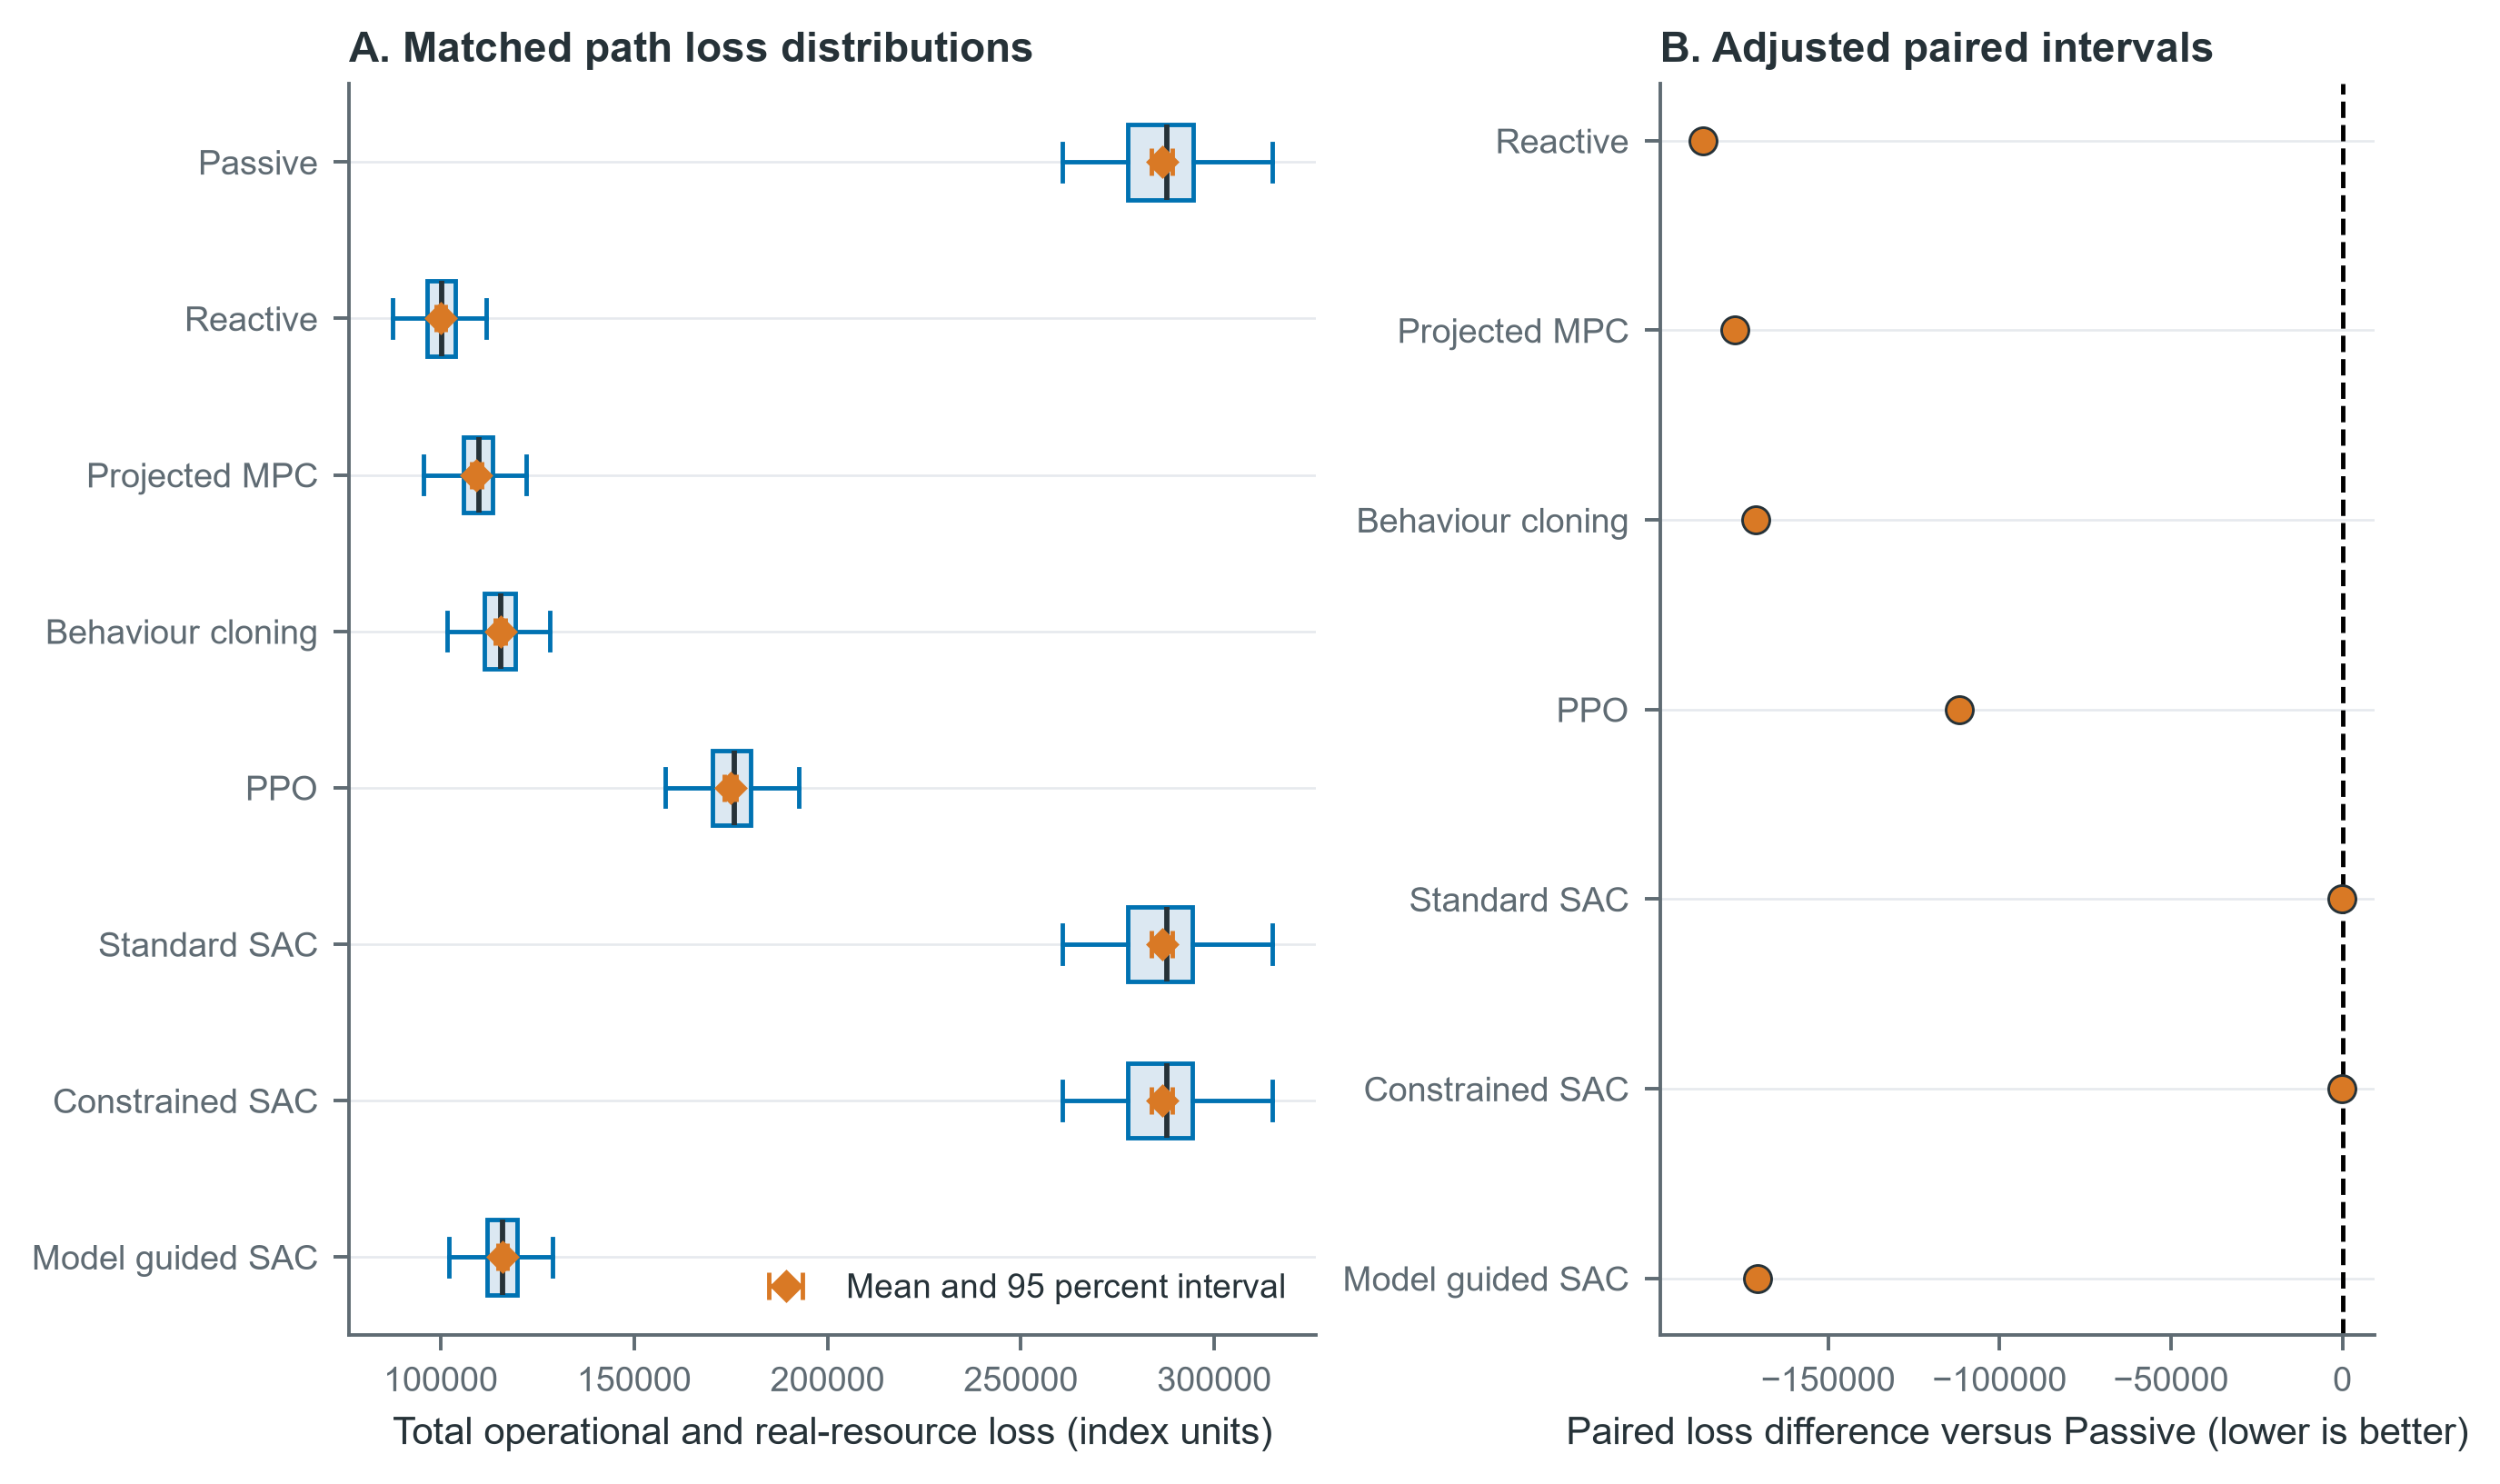
\includegraphics[width=\textwidth]{figures/figure_5_2_2a_policy_performance.png}
    \caption{Common authority policy performance and paired uncertainty}
    \label{fig:522-policy-performance}
\end{figure}

The component matrix in Figure~\ref{fig:522-loss-components} identifies waiting
as the main mechanism. Passive incurs waiting loss of 265,139.3, which is 92.5
percent of its total loss. Reactive lowers this component to 83,989.7 and also
reduces exit loss from 11,336.5 to 3,372.7. It accepts action cost of 599.9 and
higher queue, overload, and route resource losses than Passive. The waiting and
exit reductions dominate these increases. MPC records waiting loss of 90,843.2
and no cash action loss. This zero does not mean zero intervention because
release has no cash cost in the common objective. Vanilla SAC and Constrained
SAC leave waiting loss at 265,085.3 and 265,105.1. Their action costs are 3.5
and 3.4. The closed SAC updates therefore produce feasible but nearly passive
responses on these paths.

Route resource and transport loss is included in every total through
$\Delta c^{\mathrm{res}}_{kr}$ in
\cref{eq:stage-loss,eq:loss-components}. It ranges from 801.4 for Passive to
1,391.7 for MPC. The registered values zero, one, and two measure incremental
maritime lag weeks relative to Khor Fakkan. Handling, trucking, and border
increments are zero because the benchmark supplies no evidence that separates
those costs under the common topology. The component must therefore be read as
a designed real resource proxy rather than an observed monetary freight bill.
The exit component likewise contains both direct SUE exit and duration
attrition. Direct exit is small in this benchmark, so the reduction is driven
mainly by less mass ageing into attrition rather than by a policy setting an
exit quantity.

\begin{figure}[t]
    \centering
    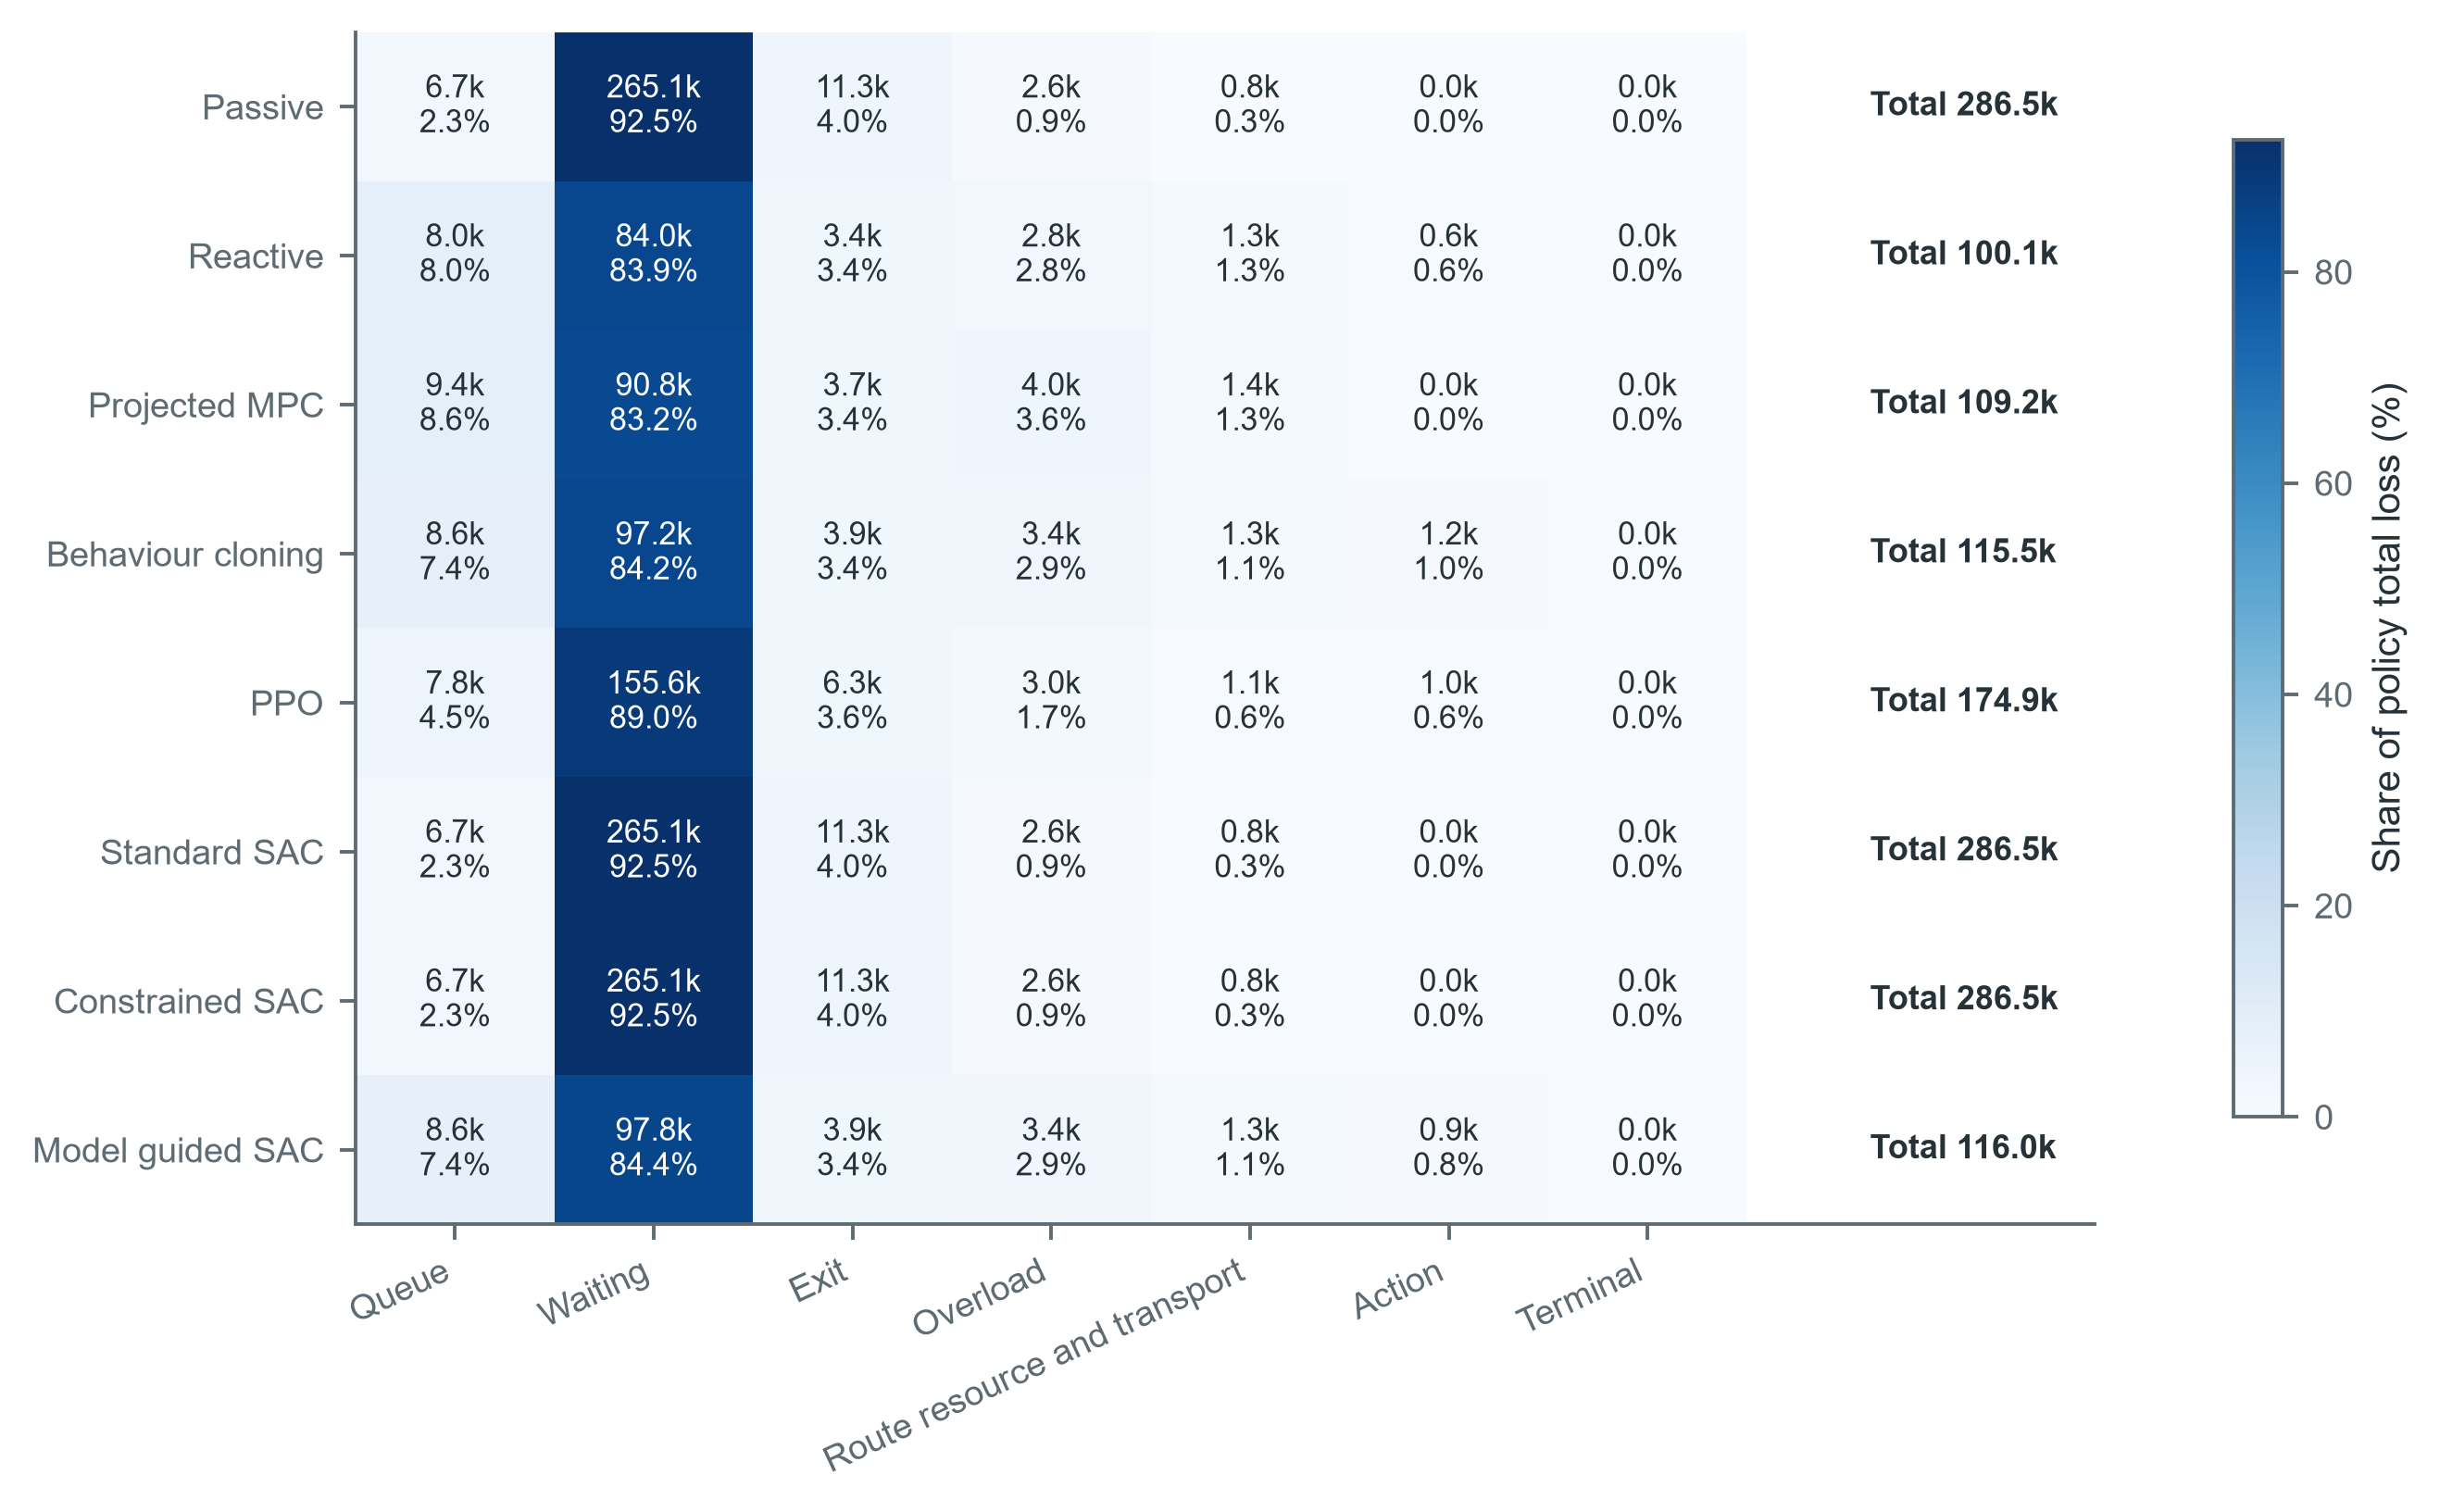
\includegraphics[width=\textwidth]{figures/figure_5_2_2b_loss_decomposition.png}
    \caption{Formal loss component matrix}
    \label{fig:522-loss-components}
\end{figure}

The clearance diagnostics rule out nonclearance as the explanation for the
loss ranking. Every trajectory clears within the 104 week continuation window,
so $\widehat P^{\mathrm{clear}}_{\pi}=1$ and no observation is right censored.
The restricted mean in \cref{eq:benchmark-clearance-metrics} is 78 weeks for
Passive, Vanilla SAC, and Constrained SAC. It is 79 weeks for Reactive, MPC,
BC, and the model guided selector. PPO is 78.996 weeks. Every mean final
outstanding mass is below $10^{-6}$ and terminal loss is zero. Lower cumulative
loss therefore does not mean faster complete clearance in this experiment.
Reactive and MPC reduce the burden carried during recovery while taking one
additional week on average to cross the strict empty tolerance.

For a regional authority, the benchmark favours an auditable current state rule
when the objective is cumulative congestion burden under the registered
resources. Reactive takes about $1.89\times10^{-4}$ seconds per decision,
compared with 10.41 seconds for MPC. The actor policies take about
$1.52\times10^{-3}$ seconds, while the model guided selector requires 3.13
seconds because it evaluates two proposals. These audited median times describe this
implementation and hardware only. The managerial result is not that learning
is unnecessary in general. It is that added complexity must demonstrate an
incremental reduction in formal waiting and propagation burden after common
authority, projection, information, and training contracts are enforced.
Clearance alone would miss this distinction. Total loss alone would miss the
one week recovery tradeoff.

The evidence boundary is narrow. The comparison is a public data calibrated
simulation with one aggregate cargo class, three gateways, one shared corridor,
a designed commitment midpoint, normalised action costs, and 88 matched test
paths.
The route resource term is not an observed transport tariff, $\gamma_I=1$ is a
design endpoint, and the physical feedback and action technology are declared
structural inputs. The benchmark neither estimates the historical committed
share nor identifies a causal port intervention effect. It also does not prove
global optimality or policy dominance under longer renewed closure, larger
gateway portfolios, different corridor bottlenecks, or alternative behavioural
and economic inputs. Those claims require the sensitivity analysis.

\FloatBarrier

\subsubsection{Action and Congestion Mechanisms}
\label{subsubsec:action-congestion-mechanisms}

The action and congestion mechanism experiment explains how the policy benchmark ranking is
produced. It asks when each formal action block becomes active, where congestion
is retained or transferred across waiting, maritime travel, and the four service
stages, and how the frozen benchmark leader changes when one action channel is
restricted. The experiment does not search for a new best policy. Its purpose is
to connect feasible actions to process outcomes while separating direct
mechanism evidence from a causal or reoptimised action value claim.

Table~\ref{tab:523-mechanism-inputs} identifies the inputs and their evidential
roles. No new external dataset or economic calibration is introduced. The
historical event and released information enter only through the accepted
benchmark paths. Requested and implemented actions, tagged states, waiting
vintages, both exit channels, capacity stocks, and loss components are replayed
through the same formal transition and policy interface.

\begingroup
\setlength{\tabcolsep}{4pt}
\begin{table}[t]
\centering
\caption{Action and congestion mechanism inputs}
\label{tab:523-mechanism-inputs}
\begin{tabular}{>{\RaggedRight\arraybackslash}p{0.20\textwidth}
                >{\RaggedRight\arraybackslash}p{0.20\textwidth}
                >{\RaggedRight\arraybackslash}p{0.27\textwidth}
                >{\RaggedRight\arraybackslash}p{0.25\textwidth}}
\toprule
Source & Retained unit & Mechanism role & Evidence boundary \\
\midrule
Frozen historical interface
& The 21 event weeks and released information accepted by the data and information validation experiment
& Common event, risk, serviceability, and blocked inflow sequence
& Observed and estimated replay under the declared transformations \\
Accepted policy benchmark
& 88 held out physical paths, three mechanism policies, requested actions, implemented actions, and frozen checkpoints
& Mechanism policy identification, matched replay, and exact input binding
& Conditional simulation evidence from the policy benchmark \\
Formal mechanism traces
& 440 policy seed path replays with source, vintage, route, capacity, queue, exit, delivery, and loss records
& Action to SUE to transition to loss reconstruction
& Auditing evidence under the formal model \\
Restricted action replay
& Full action and four restrictions on each of 88 physical paths
& Paired dependence of the frozen Reactive policy on each action channel
& Fixed policy diagnostics without reoptimisation or causal identification \\
Representative path
& One exogenous medoid selected from five features across 88 physical paths
& Fine grained route stage and provenance display
& Descriptive process evidence outside formal inference \\
\bottomrule
\end{tabular}
\end{table}
\endgroup

The main mechanism display retains Passive, Reactive as the policy benchmark mean
loss benchmark leader, and the proposed model guided constrained SAC selector.
Reactive remains a conditional benchmark leader rather than a universal
optimum. Their inherited mean losses are 286,516.53, 100,056.01, and
115,978.94. These values identify the policies whose mechanisms require
explanation and do not constitute a new ranking. All 88 physical paths support
the weekly action and aggregate outcome summaries. Learning seeds are first
averaged within path, and the bands describe path variation rather than
variation across the 21 event weeks.

The fine grained route display uses the medoid in
\cref{eq:mechanism-path-medoid}. The selected path is
\texttt{test\_017\_ebd333a3cdba}. Its standardised distance from the common
centroid is 0.5144, the smallest among the 88 candidates. Minimum serviceability
is zero on every candidate path and therefore contributes no relative
distance. Blocked mass, serviceability, and recovery geometry determine the
selection. Policy loss, action, and advantage do not. The selected path can
therefore illustrate a process but cannot replace the 88 paths used for
comparison.

The full action replay reproduces every corresponding accepted policy benchmark
outcome across 440 policy seed path trajectories. The 6,160 reproduction checks
have maximum absolute error $5.82\times10^{-11}$, well inside
$\epsilon_{\mathrm{rep}}=10^{-6}$. The four restrictions are then applied to
the raw Reactive proposal through \cref{eq:mechanism-action-restrictions}
before the common projector. No readiness sets $y_t^R=v_t^R=0$ from zero
initial readiness stock while retaining $y_t^V$. No direct capacity sets
$y_t^V=0$. Immediate release fixes $\rho_t=1$ and retains the same oldest first
operator. No disclosure sets $\lambda_t=0$ without removing the public
information system observed by the other action blocks. The physical state is
allowed to evolve after each restriction, but the Reactive policy mapping is
not retrained or reoptimised.

Reactive combines earlier release and stronger disclosure with the lowest
event end burden among the three mechanism policies. As shown in
Figure~\ref{fig:523-action-trajectories}, its mean release fraction is 0.490 and
its mean disclosure intensity is 0.609 across the decision window. The proposed
selector records 0.264 and 0.090, while Passive sets both actions to zero.
Reactive begins direct capacity orders after the initial disruption response,
exercises mature readiness when stock becomes available, and raises disclosure
to its upper bound after week ten. These actions coincide with an event week 21
burden $H_{\pi\omega t}$ of 543.29 model units, compared with 803.45 for Passive
and 611.23 for the proposed selector. The Reactive burden is therefore 32.4
percent below Passive and 11.1 percent below the proposed selector at that week.

The temporal association supports a coordinated operational interpretation.
Readiness, rapid direct capacity, waiting release, and disclosure act on
different parts of the same flow chain and should be monitored together. A port
authority that examines only a gateway queue could miss an accumulation in
external waiting or the maritime pipeline. The comparison does not assign the
32.4 percent difference to one action because the action blocks respond jointly
to a changing state and the ribbons represent variation across 88 physical paths.

\begin{figure}[t]
    \centering
    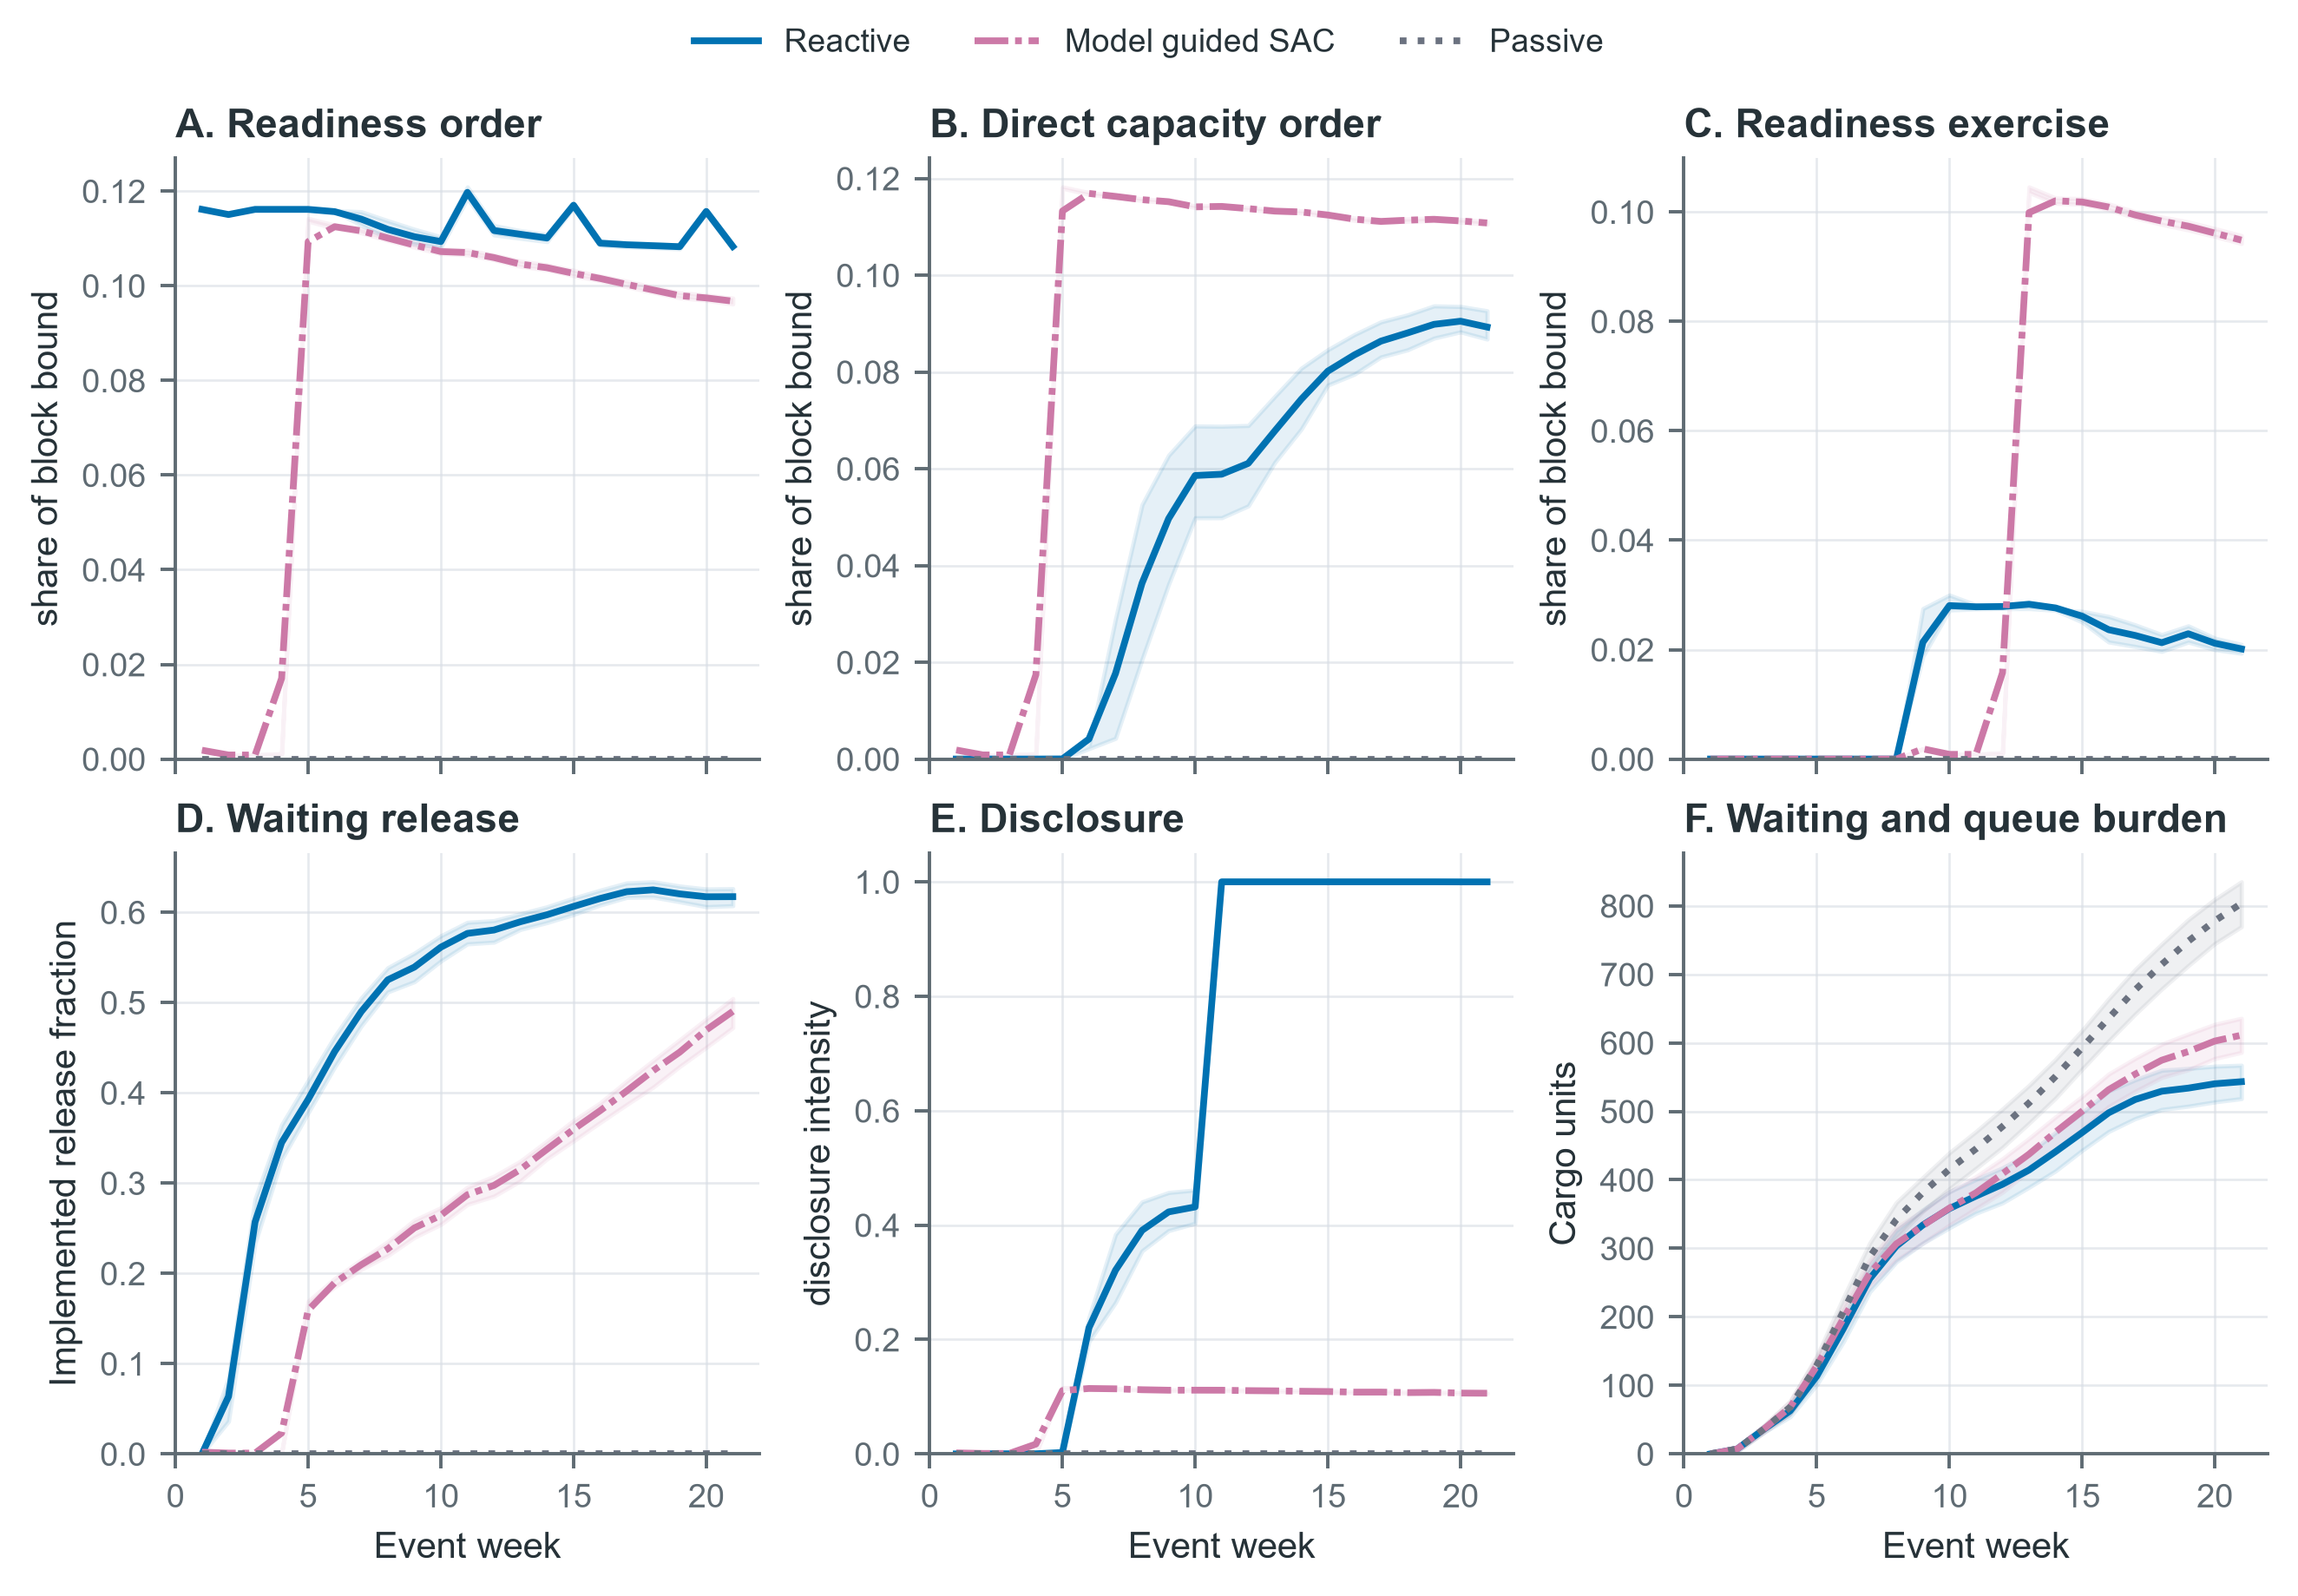
\includegraphics[width=\textwidth]{figures/figure_5_2_3a_action_congestion_trajectories.png}
    \caption{Formal action and congestion trajectories}
    \label{fig:523-action-trajectories}
\end{figure}

The proposed selector is active rather than an unused architectural layer. BC
is selected in 4,514 of 5,544 test decisions and the SAC proposal is selected
in 1,030, with no fallback. Readiness orders, direct orders, release, and
disclosure exceed $\epsilon_{\mathrm{act}}=10^{-7}$ in all 5,544 decisions.
Readiness exercise is active in 3,432 decisions because it requires mature
stock. The implemented block ranges are 48.2319 model units for readiness
orders, 49.5728 for direct orders, 44.3799 for readiness exercise, 0.620682 for
release, and 0.360943 for disclosure. This confirms that all five modules can
affect a trajectory. It does not establish that activation itself creates
economic value.
For a system operator, proposal counts are therefore a governance audit of what
the deployed controller actually uses rather than a performance criterion.

Route tags reveal that lower external waiting is accompanied by greater
maritime exposure on a longer alternative. Figure~\ref{fig:523-route-stage}
reports cumulative preservice exposure $E^{q,c}_{\pi kr}$ on the exogenous
medoid path. Under Passive, the largest adaptive route stage cell is the Khor
Fakkan berth at 439.9 model unit weeks. Under Reactive and the proposed
selector, the largest adaptive cell moves to the Sohar maritime pipeline at
1,146.3 and 1,171.1 model unit weeks. The fixed committed
itineraries do not change. Differences in their downstream cells arise from
service timing and physical propagation rather than reassignment.

The heatmap uses a square root colour scale while printing every cell in its
original unit. A dark maritime cell is not itself a port queue and can reflect
both dispatched mass and the registered route lag. The policy benchmark already
charges the corresponding route resource term, so this
transfer is not treated as costless. The mechanism explains why a coordinator
should monitor diversion from origin waiting through maritime arrival and the
shared corridor. Expanding gateway choice without observing this complete chain
could appear to relieve the focal queue while merely lengthening exposure
elsewhere.

\begin{figure}[t]
    \centering
    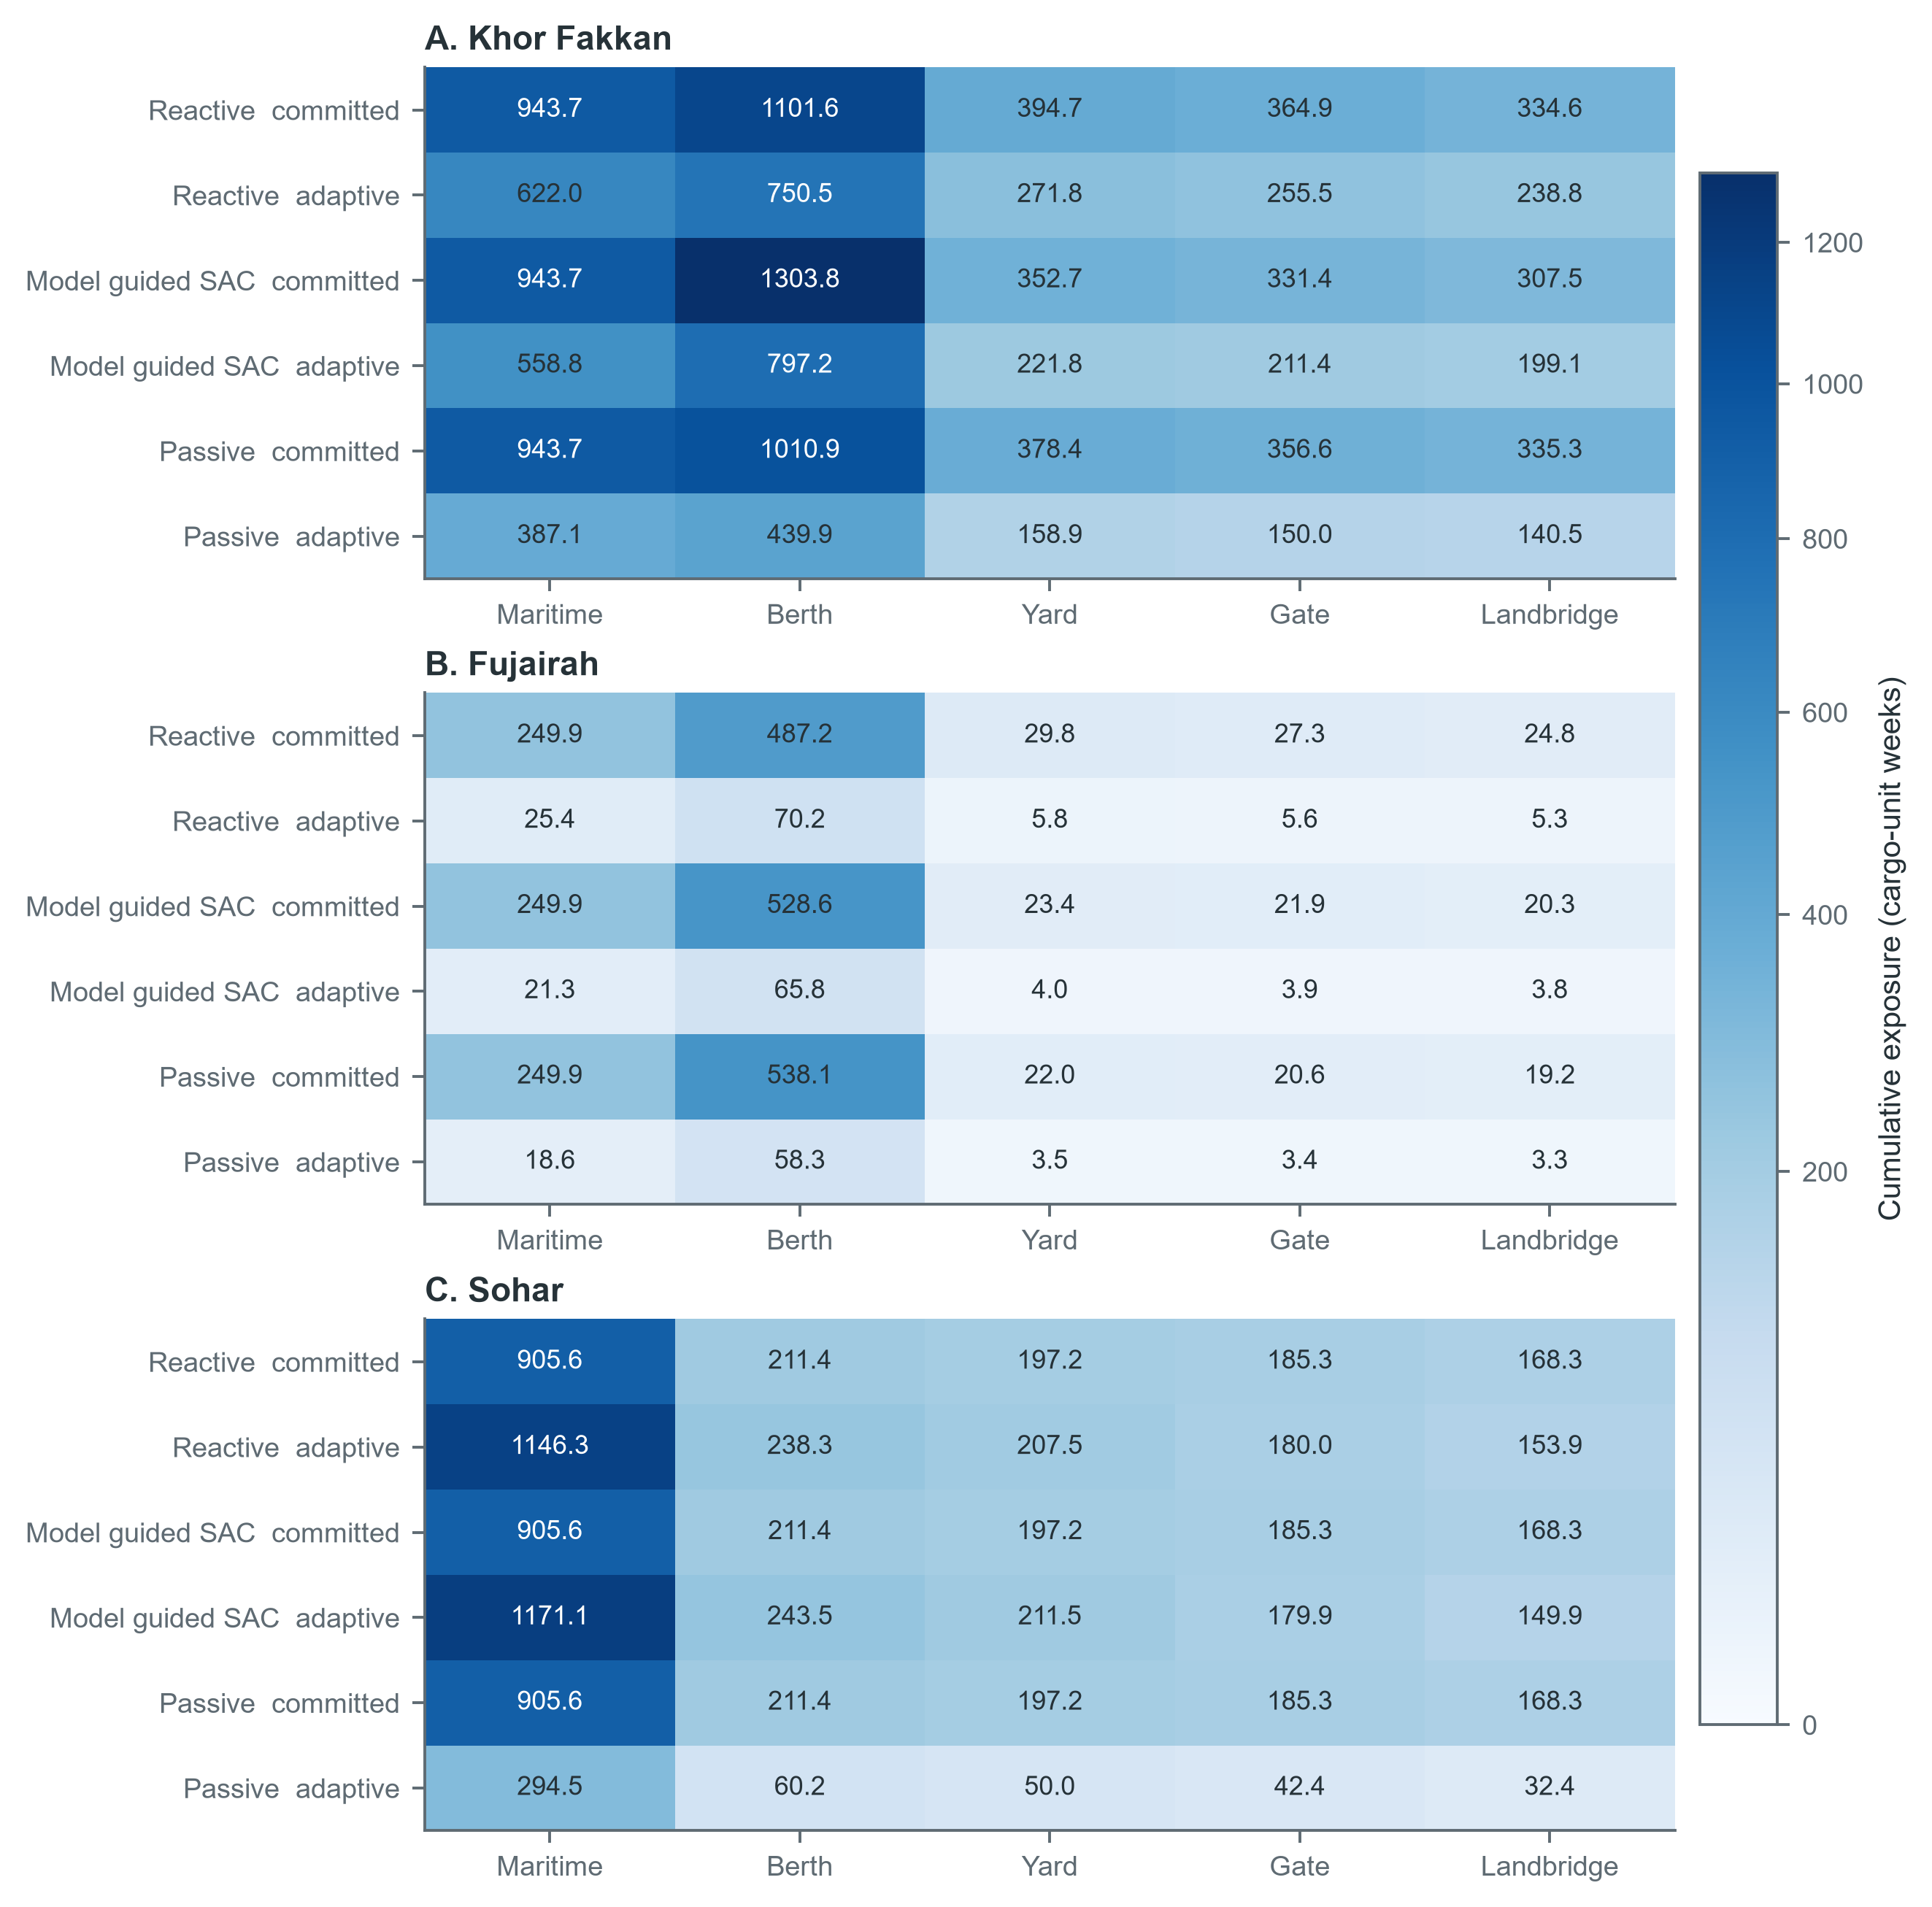
\includegraphics[width=\textwidth]{figures/figure_5_2_3b_tagged_route_stage_heatmap.png}
    \caption{Route stage exposure by dispatch provenance}
    \label{fig:523-route-stage}
\end{figure}

Direct temporary capacity is the action channel on which the frozen Reactive
policy depends most strongly in total loss terms. Figure~\ref{fig:523-restricted-actions}
reports the paired effects in \cref{eq:mechanism-paired-diagnostic}. Removing
direct capacity raises total loss by 7,166.45 with a simultaneous 95 percent
interval from 6,977.82 to 7,355.08. Waiting exposure rises by 334.73 model unit
weeks, overload rises by 274.30, duration attrition rises by 10.87, and route
resource loss rises by 100.87, despite an action cost reduction of 430.05.
Removing disclosure raises total loss by 3,973.68 with an interval from
3,839.43 to 4,107.93 and increases waiting exposure by 252.42. Removing
readiness raises total loss by 1,978.82 with an interval from 1,920.32 to
2,037.32 and increases waiting exposure by 99.34. All three total loss effects
remain resolved after Holm adjustment.

These positive differences show dependence of the frozen Reactive mapping on
the three channels under the reference network. They do not measure the value
of purchasing one more unit or the performance of a policy optimised without
that right. Within this boundary, an authority should preserve rapid direct
capacity as a contingency option and should not evaluate readiness or
disclosure only by their direct expenditure. Their operational relevance comes
from avoiding waiting age, attrition, and overload costs that exceed the saved
action cost on these paths.

Immediate release provides the important negative result. Fixing
$\rho_t=1$ lowers total loss by 4,967.21 relative to the full Reactive action,
with a simultaneous 95 percent interval from $-5{,}058.44$ to $-4{,}875.98$.
Waiting exposure falls by 445.81 model unit weeks and duration attrition falls
by 9.14. This gain is not free of physical transfer. Overload rises by 39.56,
route resource loss rises by 12.54, and action loss rises by 21.83. Direct SUE
exit rises by approximately $4.25\times10^{-6}$ model units. The waiting and
attrition reduction dominates those increases in the registered objective.

The negative sign cannot be presented as the causal value of removing release
pacing. It shows only that forcing immediate release improves the same frozen
Reactive mapping on these 88 paths after all later state responses are allowed.
The policy is not retrained within the reduced action set, and another event or
corridor state could place greater weight on the observed overload increase.
Managers should therefore treat pacing as a controller design choice that must
earn its value against an immediate release endpoint. The appropriate next step
is reoptimisation and structural stress testing, not removal of the authority
based on this diagnostic alone.

None of the four restrictions changes clearance probability and no trajectory
is right censored. The restricted mean clearance difference is zero for three
restrictions. Immediate release changes it by only $-0.011$ weeks with a
simultaneous interval from $-0.040$ to 0.018. Mean final outstanding differences
are below $8\times10^{-9}$ model units. The forest plot therefore explains
cumulative burden during disruption and recovery rather than a transfer into
nonclearance. This distinction matters because a policy can preserve eventual
clearance while imposing materially different waiting, exit, overload, route,
and action costs before the system empties.

\begin{figure}[t]
    \centering
    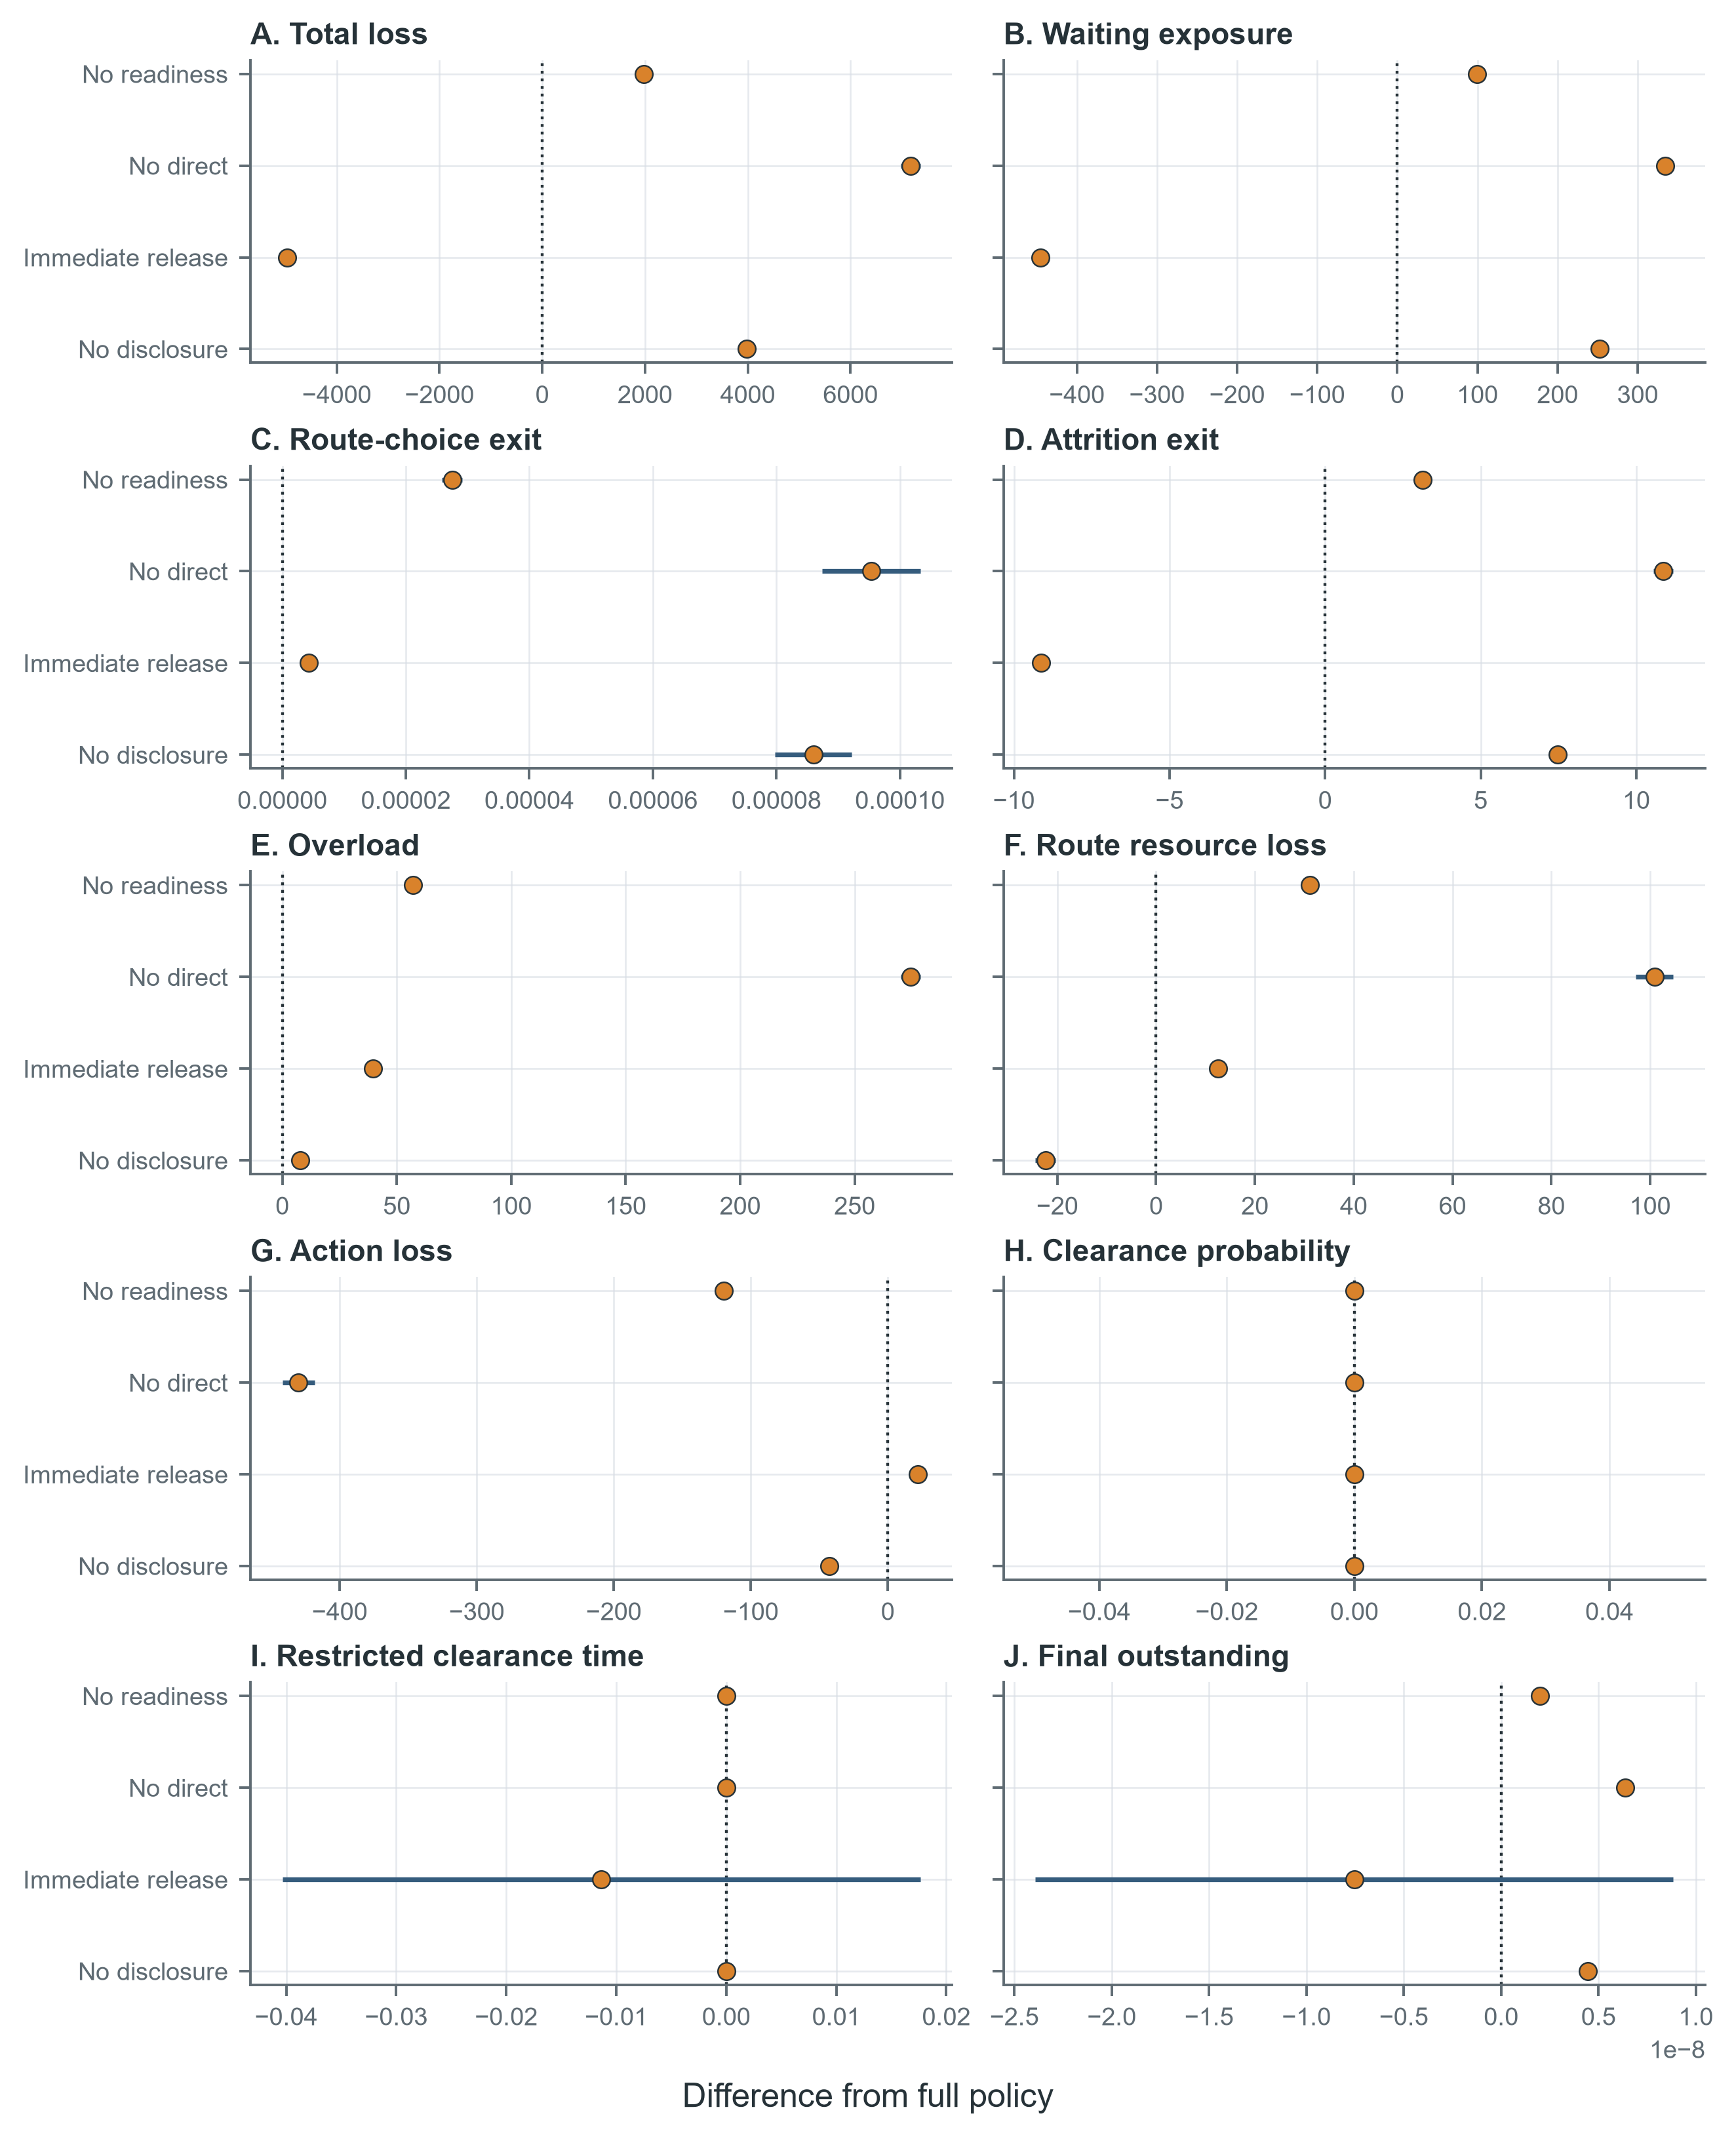
\includegraphics[width=\textwidth]{figures/figure_5_2_3c_restricted_action_forest.png}
    \caption{Fixed policy restricted action diagnostics}
    \label{fig:523-restricted-actions}
\end{figure}

All 18 blocking mechanism checks pass. The maximum transition residual is
$9.998\times10^{-7}$. Every other conservation residual is at most
$1.43\times10^{-13}$. Source choice mass, waiting vintage
identities, tagged queue conservation, provenance reconstruction, period loss,
direct procurement under no readiness, the immediate release endpoint, and the
nonaction information system under no disclosure all satisfy their registered
tolerances. The frozen inputs and regenerated outputs also pass their recorded
integrity checks. These checks make the mechanism records admissible for
interpretation. They do not by themselves validate policy effectiveness or
field execution.

The evidence boundary remains the reference simulation with one aggregate
cargo class, three gateways, one shared corridor, $\chi_{kt}=0.5$, designed
cost and action normalisations, and 88 physical paths. The medoid heatmap is a
single descriptive slice. Its provenance ledger is an accounting decomposition
that neither augments the formal state nor feeds information to a policy. The
restricted comparisons preserve one Reactive mapping and are neither causal
marginal values nor reoptimised action right values. PortWatch activity also
remains an AIS derived activity proxy rather than observed diversion cargo.
Longer renewed closure, different commitment, larger gateway portfolios, and
alternative corridor or behavioural conditions remain outside this experiment
and are addressed through the sensitivity analysis.

\FloatBarrier

\subsubsection{Risk Information and Capacity Preparation}
\label{subsubsec:released-risk-capacity}

The risk information and capacity preparation experiment asks whether legally released geopolitical risk
information improves the proposed controller after the information regime is
matched during training, whether earlier release of the same packet creates
timing value, and whether readiness and direct procurement provide complementary
capacity rights. These questions are distinct. Information value requires
condition specific optimisation. Substituting information into one frozen
checkpoint measures only signal responsiveness. Capacity portfolio value
requires each reduced action set to be optimised again.

Table~\ref{tab:524-information-inputs} records the inputs and their evidential
roles. No new external observation or economic coefficient is introduced. The
experiment inherits the accepted monthly risk model and release clock from
the data and information validation experiment and the physical paths, policy
architecture, transitions, loss, and clearance rule from the policy benchmark.

\begingroup
\setlength{\tabcolsep}{4pt}
\begin{table}[t]
\centering
\caption{Released information and capacity preparation inputs}
\label{tab:524-information-inputs}
\begin{tabular}{>{\RaggedRight\arraybackslash}p{0.20\textwidth}
                >{\RaggedRight\arraybackslash}p{0.21\textwidth}
                >{\RaggedRight\arraybackslash}p{0.27\textwidth}
                >{\RaggedRight\arraybackslash}p{0.24\textwidth}}
\toprule
Source & Retained unit & Experimental role & Evidence boundary \\
\midrule
Accepted risk interface
& The estimated transition matrix, training stationary distribution, released monthly beliefs, and Monday information clock
& Construction of $I_0$, $I_F$, $I_L$, and $I_O$ through \cref{eq:information-regimes-524}
& Estimated risk state information without a closure label \\
Accepted policy benchmark
& Eighty eight held out physical paths, three learning seeds, common model transitions, and the complete operational loss
& Matched evaluation and the unchanged $I_L$ controller with both capacity rights
& Conditional simulation evidence under the reference network \\
Release timing cases
& Historical release $G_H$, sufficient release $G_T$, insufficient release $G_L$, and false warning $G_{\mathrm{FW}}$
& Timing gaps from \cref{eq:information-release-gap-524} and an eight week preparation window
& One historical information replay and three designed timing stresses \\
Controller conditions
& Four information regimes, four capacity right sets, and one fixed checkpoint substitution
& Reoptimised information and rights comparisons with a separate responsiveness diagnostic
& Algorithm value separated from fixed policy response \\
Formal outcome records
& Actions, capacity stocks, tagged transitions, clearance, and every loss component
& Information value, capacity right value, mechanism tracing, and identity checks
& Model based outcomes rather than realised port intervention effects \\
\bottomrule
\end{tabular}
\end{table}
\endgroup

The primary information layer trains and selects the proposed controller under
each regime in \cref{eq:information-regimes-524}. The accepted $I_L$ controller
with both capacity rights remains the policy benchmark anchor because it was
already trained under that exact interface. Controllers for $I_0$, $I_F$, and
$I_O$ are trained from their own training and validation paths without observing
test paths. The oracle controller receives realised current and maturity status.
Its information set is theoretically dominant but its trained performance must
still be verified. The same $I_L$ checkpoint is evaluated under $I_0$, $I_F$,
and $I_L$ to test whether the architecture responds to a changed signal. This
second layer is not used to estimate information value.

Every case uses 88 physical paths and three learning seeds. Seeds are averaged
within path before paired inference, and simultaneous intervals follow
\cref{eq:information-inference-524}. The primary information and capacity right
layers each contain 1,408 path records. The fixed checkpoint layer contains
1,056 path records. Together the experiment retains 11,616 seed replications
and 336,864 weekly records. The eight preparation Mondays precede the accepted
21 event weeks, and clearance retains the 104 week follow up rule. The $G_H$
case preserves the public release dates. The $G_T$ case moves the last event
antecedent packet to the Monday that exactly permits eight week readiness
maturity. The $G_L$ case releases the same packet one week later. The
$G_{\mathrm{FW}}$ case uses the sufficient release schedule with normal demand
and full serviceability. Event physics, demand residuals, operational scenario
construction, market information, budgets, and random seed indices remain
matched where the estimand requires them.

Lead aligned information improves the reoptimised controller under the
historical release path, whereas current filtering alone slightly worsens it.
Figure~\ref{fig:524-information-value} reports the effects in
\cref{eq:information-capacity-values-524}. A positive value denotes a loss
reduction. The $I_F$ value is $-86.41$ model loss units under $G_H$, with a
simultaneous 95 percent interval from $-97.14$ to $-75.67$. Current filtering
therefore increases loss by 86.41 relative to $I_0$. The $I_L$ value is
$2{,}644.63$, with an interval from $2{,}558.79$ to $2{,}730.47$. Its incremental
value relative to $I_F$ is $2{,}731.03$, with an interval from $2{,}651.21$ to
$2{,}810.86$. All three comparisons remain resolved after Holm adjustment. The
contrast shows that a current risk coordinate can direct costly preparation
without improving the complete system, while alignment with readiness maturity
can change that decision. A coordinator should therefore assess released risk
information against the resource lead and the complete operational loss rather
than procure a current state signal on filtering accuracy alone.

The trained oracle controller reduces loss by only 134.19 relative to $I_0$,
with a simultaneous interval from 104.23 to 164.14. More importantly, its
realised oracle gap $G^O$ is $-2{,}510.44$, with an interval from $-2{,}597.47$
to $-2{,}423.41$. The negative gap means that the trained oracle controller has
higher loss than the lead aligned controller even though its information set is
theoretically dominant. This inversion is an optimisation or training
limitation. It is not evidence that perfect information is intrinsically
harmful and it cannot be presented as an attained upper bound. The oracle
result therefore diagnoses the distance between information availability and
controller attainment rather than a procurable managerial benefit.

\begin{figure}[t]
    \centering
    
\includegraphics[width=\textwidth]{figures/figure_5_2_4a_released_information_value.pdf}
    \caption{Released information value and policy response}
    \label{fig:524-information-value}
\end{figure}

Moving the target packet changes neither main information effect materially.
Across $G_H$, $G_T$, and $G_L$, the maximum difference among the reported
information effects is 0.010 model loss units. The shifted packet contains
almost no current high risk probability, while its maturity projection remains
close to the 0.116 training stationary share. Earlier availability therefore
does not create a materially different decision input in this construction.
This is a negative timing result for the released content and controller
studied here. It does not imply that earlier public information is generally
valueless. Authorities should first establish that a packet changes the lead
relevant probability before paying for faster release or advance capacity on
timing grounds.

The fixed checkpoint panel in Figure~\ref{fig:524-information-value} provides a
separate interface check. With the identical $I_L$ controller, replacing $I_0$
by $I_F$ reduces loss by 242.87 with an interval from 227.99 to 257.75. Replacing
$I_0$ by $I_L$ reduces loss by 192.78 with an interval from 179.08 to 206.48.
The checkpoint is therefore responsive to both signal coordinates. The
positive response under the fixed checkpoint does not contradict the negative
reoptimised $I_F$ value because the policy and evaluation information are not
matched in this diagnostic. These effects demonstrate interface use and
response outside the selected information condition. They do not measure
information value or policy superiority.

The false warning construction produces another necessary qualification. The
mean costs in \cref{eq:information-diagnostics-524} are $-0.082$ for $I_F$,
$7.072$ for $I_L$, and $12.915$ for $I_O$. Positive values record added loss
when no physical disruption occurs. Ten false warning comparisons have zero or
numerically negligible across path variance, which produces zero width or
nearly zero width intervals. Their deterministic matched differences describe
this designed case. Nominal zero $p$ values from these comparisons are not
conventional sampling evidence.

The historical timing trace clarifies why information availability and useful
capacity are not the same object. Figure~\ref{fig:524-capacity-timing} follows
the exogenous physical path medoid selected by
\cref{eq:mechanism-path-medoid} under $G_H$, $I_L$, and both capacity rights.
The accepted medoid is selected only from blocked mass, serviceability, and
recovery features and has standardised distance 0.5144 from the common centre.
It is a mechanism display and does not replace the 88 paths used for inference.

Before event onset, the current high risk probability is effectively zero and
the lead aligned probability remains close to 0.116. Small readiness orders
placed eight weeks earlier begin to mature immediately before onset and are
first exercised when the event begins. Larger readiness orders start on 23
March and mature from 11 May, while direct orders arrive in their order week.
The trace therefore verifies the distinct eight week and zero week delivery
rules. It also shows that most capacity expansion follows realised congestion
rather than the historical warning packet. For an authority, information
release and capacity delivery must be audited as one dated chain. A signal that
arrives earlier has no operational value unless it changes an admissible order
before the relevant resource lead closes.

\begin{figure}[t]
    \centering
    
\includegraphics[width=\textwidth]{figures/figure_5_2_4b_release_capacity_timing.pdf}
    \caption{Information release and capacity preparation}
    \label{fig:524-capacity-timing}
\end{figure}

The same trace exposes the remaining physical burden. Four stage queues continue
to accumulate while usable temporary capacity rises, and blocked cargo remains
positive across the event window. Capacity can relieve a local resource without
eliminating external waiting or the cost of acquiring that capacity. A port
coordinator should therefore monitor order date, maturity, exercise, immediate
delivery, external waiting, and the full queue chain together. The
representative trace does not identify the marginal value of either action
because it is one realised path from a jointly responding policy.

Readiness and direct procurement are complementary under the historical release
case and the reference prices and leads. Figure~\ref{fig:524-capacity-portfolio}
applies the rights restrictions in \cref{eq:capacity-rights-524} and reoptimises
every condition. Under $G_H$, mean total loss is 115,985.81 with both rights,
119,181.59 with readiness only, 120,582.20 with direct procurement only, and
120,747.11 with neither right. Adding readiness when direct procurement exists
has value $V_{R\mid D}=4{,}596.39$ with a simultaneous interval from 4,501.58 to
4,691.20. Adding direct procurement when readiness exists has value
$V_{D\mid R}=3{,}195.78$ with an interval from 3,105.80 to 3,285.76. The
combination effect is $S_{RD}=3{,}030.88$ with an interval from 2,938.16 to
3,123.60. All three differences remain resolved after Holm adjustment.

The complete loss decomposition explains the complementarity. Relative to
neither right, both rights reduce waiting loss by 4,783.93, queue loss by 393.00,
attrition exit loss by 195.88, overload loss by 302.47, and route resource loss
by 27.71. These reductions exceed the additional action loss of 941.70. The two
rights are valuable together because the immediate resource covers the period
before readiness matures, while the prepared resource supports later weeks.
Total loss includes transportation related route resource loss as well as
queue, waiting, both exit channels, overload, action, and terminal components.
The finding is therefore not produced by omitting transportation cost.

\begin{figure}[t]
    \centering
    
\includegraphics[width=\textwidth]{figures/figure_5_2_4c_capacity_portfolio.pdf}
    \caption{Readiness and direct procurement portfolio}
    \label{fig:524-capacity-portfolio}
\end{figure}

The capacity relation reverses under $G_{\mathrm{FW}}$. The three right effects
$V_{R\mid D}$, $V_{D\mid R}$, and $S_{RD}$ become $-9.39$, $-20.82$, and
$-6.17$. With no disruption, the capacity rights create preparation cost
without congestion relief. This result is distinct from the false warning
information cost, which compares information regimes while holding the rights
case fixed. Managers should therefore preserve access to both instruments when
the disruption case and reference cost structure apply, but condition exercise
and direct procurement on the physical burden rather than activate the
portfolio for every warning. The conclusion is conditional on the designed
unit costs, eight week readiness lead, zero lead direct procurement, common
budget, and trained controllers. It is not a field estimate of procurement
prices or universal technological complementarity.

All 40 registered contrast precision targets are met. The largest achieved
half width is 64.03 against the target 2,255.64. Every evaluated path clears
within the follow up horizon, no trajectory is right censored, and terminal loss
is zero. Independent reconstruction matches all paired interval endpoints
within $4.04\times10^{-12}$. The maximum transition residual is
$9.99991\times10^{-7}$ against the $10^{-6}$ tolerance, and the maximum loss
closure error is $2.91\times10^{-11}$. The accepted policy benchmark anchor is
reproduced within $1.46\times10^{-11}$. These checks establish admissibility of
the reported comparisons rather than field effectiveness.

The evidence boundary is a historical release replay combined with three
designed timing stresses, 88 physical paths, one aggregate cargo class, three
gateways, one shared corridor, $\chi_{kt}=0.5$, and the reference economic and
capacity normalisations. The HMM supplies a geopolitical risk state belief and
a maturity aligned state forecast. It does not predict an exact closure date.
The fixed checkpoint layer is responsiveness evidence only. The oracle
information set is unattainable and its trained controller does not attain the
theoretical performance bound. Capacity right effects remain conditional
simulation results. Alternative resource costs, longer direct lead, readiness
expiry, renewed closure, and network expansion can change these relations and
remain for the sensitivity analysis.

\FloatBarrier

\subsubsection{Computational Acceptance}
\label{subsubsec:computational-methodological-acceptance}

The computational acceptance experiment asks whether the computations reported by the preceding
benchmark experiments preserve the formal model and solution contract. It separates
engineering connectivity, numerical validity, method implementation, and
experimental precision. This separation is necessary because a small solver
residual cannot compensate for an incomplete learning update, and a correct
implementation cannot compensate for imprecise policy evidence. Overall
acceptance therefore follows the noncompensatory rule in
\cref{eq:method-acceptance-525}.

Table~\ref{tab:525-acceptance-inputs} records the data sources and their
evidential roles. No new observation, behavioural coefficient, cost weight, or
physical capacity is introduced. The experiment uses the accepted released
information interface from the data and information validation experiment and
the frozen paths, checkpoints, actions, physical transitions, and losses from
the policy, mechanism, and risk information experiments.

\begingroup
\setlength{\tabcolsep}{4pt}
\begin{table}[t]
\centering
\caption{Computational and methodological acceptance inputs}
\label{tab:525-acceptance-inputs}
\begin{tabular}{>{\RaggedRight\arraybackslash}p{0.20\textwidth}
                >{\RaggedRight\arraybackslash}p{0.22\textwidth}
                >{\RaggedRight\arraybackslash}p{0.27\textwidth}
                >{\RaggedRight\arraybackslash}p{0.23\textwidth}}
\toprule
Source & Retained unit & Experimental role & Evidence boundary \\
\midrule
Accepted upstream interfaces
& Released information records, 88 physical paths, 1,584 policy path records, checkpoints, and run manifests
& Identity, chronology, matched path, clearance, precision, and reproducibility audits
& Accepted inputs rather than an independent reestimation \\
Production numerical records
& Requested and applied actions, SUE residuals, tagged states, capacity pipelines, loss terms, and terminal stocks
& Projection, nonanticipativity, conservation, travel time, capacity timing, and loss closure checks
& Tested production trajectories under the registered tolerances \\
Controlled solver cases
& Three production lower level problems and one nested control case with seven candidates
& RC MSA comparison, expected objective reproduction, and finite lattice minimisation
& Numerical diagnostics rather than a policy comparison or continuous global optimisation \\
Learning and selector records
& BC records, complete SAC update traces, validation checkpoints, paired proposal scores, and selected proposals
& Twelve SAC contracts, validation selection, mechanical proposal selection, and candidate set regret
& Internal implementation and frozen candidate evidence rather than global learning optimality \\
Contract reinforcement records
& Complete master support histories, disclosure reference calls with $a_t^{-I}$, 105 waiting vintage balances, nested module certificates, and numerical equivalence records
& Master choice distance, information exclusion, age retention, nested module reconstruction, and repair equivalence checks
& Acceptance certificates rather than new observations, parameters, or policy outcomes \\
Execution records
& Recorded call times, software version, declared processor, deterministic seeds, and output hashes
& Computational profile and replay identity
& One machine without an external operating deadline or retained historical training memory \\
\bottomrule
\end{tabular}
\end{table}
\endgroup

The settings follow Table~\ref{tab:parameter-register-84}. Each of the three
lower level cases is solved by RC MSA and conventional MSA on the identical
fixed point problem with tolerance $10^{-6}$ and a 500 iteration cap. RC MSA
uses the registered residual controlled steps, while conventional MSA uses
$1/(n+1)$. The action audit applies the registered weighted Euclidean
projection. The control audit independently recalculates
\cref{eq:mpc-objective} for seven frozen action candidates, three common
scenarios, and the eight week horizon. The learning audit checks stochastic
reparameterisation, both reward critics, the constraint critic, the actor mean
and log standard deviation, the entropy term and temperature, the constraint
dual, the projection Jacobian, finite differences, and validation checkpoint
selection. Three learning seeds are first averaged within each physical path.
The selector audit then applies \cref{eq:two-proposal-selector} without an added
score or discretionary weight. Five further checks reconstruct the historical
distance on the full master choice set, enforce $a_t^{-I}$ at the disclosure
reference interface, preserve every waiting vintage without an age reset,
retain every nested module record, and compare accepted scientific quantities
before and after the core repair.

RC MSA satisfies the common tolerance in all three production cases.
Figure~\ref{fig:525-numerical-convergence} reports convergence after 7, 7, and
10 iterations, with a maximum terminal residual of
$7.83\times10^{-7}$. Conventional MSA does not satisfy the same tolerance in
any case within 500 iterations. Its terminal residuals range from
$5.27\times10^{-6}$ to $1.68\times10^{-5}$. This is negative evidence for the
conventional update under the common cap, but three controlled cases do not
establish universal RC MSA superiority.

The same figure shows the nested control audit. All seven expected objectives
are reproduced with zero numerical difference, and the recorded control is the
mechanical minimiser of the frozen lattice. The zero action candidate has the
minimum objective of 41.5772 in this controlled case. One, two, and three
scenario prefixes select the same candidate and reproduce this objective. This
prefix result checks the implemented nesting only. It does not establish that
three scenarios are sufficient in other states or that the finite candidate
minimum is the continuous action optimum. The managerial value is procedural.
An authority can reject an action when the equilibrium residual or nested
objective cannot be reproduced before implementation.

\begin{figure}[t]
    \centering
    
\includegraphics[width=\textwidth]{figures/figure_5_2_5a_numerical_convergence.pdf}
    \caption{Equilibrium convergence and nested control acceptance}
    \label{fig:525-numerical-convergence}
\end{figure}

Figure~\ref{fig:525-learning-selector} closes the learning contract that supports
the benchmark checkpoints. All twelve critical SAC checks pass. They jointly
verify the stochastic actor, twin reward critics, constraint critic, mean and
log standard deviation updates, entropy contribution, adaptive temperature,
constraint dual, projected gradient, finite difference reconstruction, and
validation based checkpoint selection. The maximum relative actor gradient
error is $1.75\times10^{-11}$, and the maximum projection Jacobian error is
$6.35\times10^{-13}$. These checks establish correspondence with the formal
learning equations. They do not imply that the trained policy reaches a
global optimum or outperforms the operational comparators.

The selector follows its formal score in all 5,670 recorded decisions. This
total comprises 126 validation decisions and the 5,544 held out test decisions
reported in the policy benchmark and mechanism experiment. On the test paths, the selector chooses
the BC proposal 4,514 times and the SAC proposal 1,030 times, with no fallback.
Mechanical compliance does not imply that either proposal is good. Relative to
the better frozen candidate after each path is realised, selector regret has a
mean of 510.46 loss units and ranges from 157.35 to 872.35. This retained
negative result explains why model guided constrained SAC does not improve on
BC in the policy benchmark. The managerial implication is that an auditable selector
still requires a strong candidate set and an accurate nested score. Governance
of the choice rule cannot substitute for candidate quality.

\begin{figure}[t]
    \centering
    
\includegraphics[width=\textwidth]{figures/figure_5_2_5b_learning_selector.pdf}
    \caption{Learning contract and proposal selector acceptance}
    \label{fig:525-learning-selector}
\end{figure}

All 32 critical method contracts pass, as shown in
Figure~\ref{fig:525-contract-runtime}. The largest normalised residual is 0.783
for RC MSA and remains below its acceptance boundary of one. The 1,408 replay
checks that bind the policy, mechanism, and risk information experiments have a maximum difference of
$5.82\times10^{-11}$. Maximum tagged mass and loss closure errors are
$5.68\times10^{-14}$ and $2.91\times10^{-10}$. Thus the accepted figures and
statistics are connected to the same released information, projected actions,
tagged transitions, capacity timing, and complete loss account used by the
model.

The five reinforcement contracts also pass. The master choice and disclosure
reference errors are zero. All 105 waiting vintage balances pass, and the
independent age zero no reset identity has zero error. The largest nested module certificate error is
$1.71\times10^{-13}$. RC MSA diagnostics and MPC candidate objectives remain
numerically identical before and after the repair, while the largest upstream
anchor difference is $5.82\times10^{-11}$. These results show that the stronger
audit closes previously unrecorded contracts without changing the accepted
benchmark evidence. They do not provide an additional policy comparison.

The experimental evidence layer also passes. All 88 required physical paths
are executed, and all seven registered precision contrasts satisfy the target
in \cref{eq:benchmark-path-precision}. The maximum paired half width is
2,237.54, below the target of 2,255.64. None of the 1,584 policy paths is right
censored. This supports the finite confidence statements already reported in
the policy benchmark. It does not remove the conditional simulation boundary or turn a
confidence set leader into a universally optimal policy.

The runtime panel provides a descriptive burden profile for Python 3.12.13 under
Windows 11 on the declared AMD64 machine. Median and 95 percent decision times
are 10.41 and 16.68 seconds for projected stochastic MPC, and 3.13 and 5.04
seconds for the model guided selector. The individual learned actors require
about $1.52\times10^{-3}$ seconds at the median. Reactive requires about
$1.89\times10^{-4}$ seconds. These values identify the nested objective as the
main online burden. They do not establish real time operability because no
external response deadline is registered.

\begin{figure}[t]
    \centering
    
\includegraphics[width=\textwidth]{figures/figure_5_2_5c_contract_runtime.pdf}
    \caption{Critical method contracts, upstream reproduction, and runtime}
    \label{fig:525-contract-runtime}
\end{figure}

Engineering acceptance, numerical acceptance, method contract acceptance, and
experimental evidence acceptance all pass. Overall acceptance therefore also
passes under \cref{eq:method-acceptance-525}. Three noncritical diagnostics
remain explicitly untested. They are the SLSQP dual and KKT multipliers, BC
validation error by action coordinate, and historical training wall time and
peak memory. No substitute values are constructed. These omissions do not
invalidate the registered critical contracts, but they prevent a claim of
comprehensive diagnostic instrumentation.

The experiment boundary is the frozen benchmark production chain, 32
critical contracts, three controlled equilibrium problems, one seven candidate
control lattice, two selector proposals, 88 physical paths, and one runtime
environment. Acceptance concerns implementation connectivity, registered
numerical conditions, and attained path precision. It does not establish
global optimality, universal policy superiority, causal effects at real ports,
or real time deployability.

Taken together, the benchmark experiments follow a single evidence chain. Data
and information validation establishes the event input and released information
clock. The policy benchmark provides the conditional common authority comparison.
The mechanism experiment identifies action and congestion processes without
reranking policies. The risk information experiment separates released
information, fixed checkpoint response, and capacity rights. Computational
acceptance verifies that these claims originate from the registered
model and attain the declared numerical and path precision conditions. Negative
results for the third month HMM score, learned policy performance, immediate
release diagnostic, trained oracle, conventional MSA, and selector regret are
retained. The sensitivity analysis therefore tests structural boundaries rather than using
method acceptance to extend the empirical claims.

\FloatBarrier
\subsection{Sensitivity Analysis}
\label{subsec:sensitivity-analysis}

\subsubsection{Commitment Sensitivity}
\label{subsubsec:commitment-sensitivity}

The commitment sensitivity experiment asks how itinerary lock changes the
remaining scope for common authority coordination. The structural share
$\chi$ assigns only each newly blocked cohort to committed dispatch or adaptive
choice. It is not estimated from the historical event. The experiment therefore
tests controllability over the complete admissible domain rather than treating
the neutral benchmark midpoint as an observed cargo characteristic.

Table~\ref{tab:531-commitment-inputs} records the data and experimental inputs.
No new observation is added. The accepted historical interface supplies the
same event and released information path, while the accepted path builder
supplies the same physical disturbances for every commitment value and policy.

\begingroup
\setlength{\tabcolsep}{4pt}
\begin{table}[t]
\centering
\caption{Commitment sensitivity inputs}
\label{tab:531-commitment-inputs}
\begin{tabular}{>{\RaggedRight\arraybackslash}p{0.20\textwidth}
                >{\RaggedRight\arraybackslash}p{0.22\textwidth}
                >{\RaggedRight\arraybackslash}p{0.27\textwidth}
                >{\RaggedRight\arraybackslash}p{0.23\textwidth}}
\toprule
Source & Retained unit & Experimental role & Evidence boundary \\
\midrule
Accepted historical interface
& Twenty one weekly event records with released risk states and event inputs
& Common historical clock, serviceability, blocked flow, and released information
& Frozen input rather than a new event estimate or commitment observation \\
Matched physical paths
& Eighty eight held out paths containing common residual blocks and service trajectories
& Path paired policy evaluation in every commitment cell
& Public data calibrated simulation rather than independent realised disruptions \\
Registered network and authority
& Three gateways, the common 34 coordinate action, capacity pipelines, costs, and clearance rule
& Identical physical and decision contract across the grid
& Conditional evidence for the declared network and common authority \\
Commitment and training register
& Nine commitment values, common seed indices, condition specific teacher data, and 81 checkpoint records
& Cohort splitting, retraining, validation selection, provenance conservation, and replay identity
& Designed structural variation with no reuse of benchmark learning checkpoints \\
\bottomrule
\end{tabular}
\end{table}
\endgroup

The grid is
$\chi\in\{0,0.125,0.25,0.375,0.50,0.625,0.75,0.875,1\}$. The five point
endpoint and quartile design and the four intervening eighth points were all
registered before outcomes were inspected. The split and provenance metrics
follow \cref{eq:commitment-sensitivity-metrics}. Passive, Reactive, projected
stochastic MPC, BC, and model guided constrained SAC form the comparison set.
Teacher data, BC, and constrained SAC are regenerated within every commitment
cell. Validation precedes test evaluation, and no accepted benchmark checkpoint
is reused. The design produces 7,128 policy path seed runs. The three learning
seeds are averaged within each path before inference.

Endpoint variance is evaluated against both Passive and Reactive for each of
the other four policies. This gives 16 registered precision contrasts. Their
largest required count is 88 paths, so the common grid does not expand to the
cap of 196. Within each commitment cell, let
\begin{equation}
 \widehat\pi_{\chi}
 =\argmin_{\pi\in\Pi^C}\frac{1}{N_{\mathrm{path}}}
 \sum_{\omega}\bar J^{\mathrm{op}}_{\pi\omega}(\chi),
 \qquad
 \mathcal C^{\mathrm{best}}_{\chi}
 =\left\{\pi\in\Pi^C:
 L^{\mathrm{sim}}_{\pi,\widehat\pi_{\chi}}(\chi)\leq0\right\},
 \label{eq:commitment-confidence-set}
\end{equation}
where $L^{\mathrm{sim}}$ is the lower bound of the simultaneous interval for
the path paired loss difference from the sample leader. Holm adjusted tests and
Bonferroni intervals are calculated within each registered family.

Reactive is the sample loss leader and the sole member of
$\mathcal C^{\mathrm{best}}_{\chi}$ in all nine cells, as shown in
Figure~\ref{fig:531-loss-regret}. At $\chi=0$, Reactive reduces loss relative
to Passive by 223,726.63 units, with a simultaneous interval from 221,400.35 to
226,052.92 for the reduction. At $\chi=1$, the corresponding reduction narrows
to 6,138.54, with an interval from 5,884.33 to 6,392.74. Thus the value of
adaptive coordination is greatest when newly blocked cargo remains eligible for
choice and contracts progressively remove that discretion. An authority should
therefore establish the existing itinerary lock before transferring a policy
comparison to a new event. This ranking remains conditional on the five declared
policies, network, costs, and matched paths.

At the reference midpoint, mean losses are 100,056.01 for Reactive, 109,237.91
for MPC, 115,923.55 for BC, 116,385.41 for model guided constrained SAC, and
286,516.53 for Passive. Passive, Reactive, and MPC preserve their deterministic
benchmark anchors. The learned values are condition specific retraining results
rather than reproductions of the benchmark checkpoints. This distinction
prevents a small checkpoint difference from being interpreted as a change in
the structural policy ordering.

\begin{figure}[t]
    \centering
    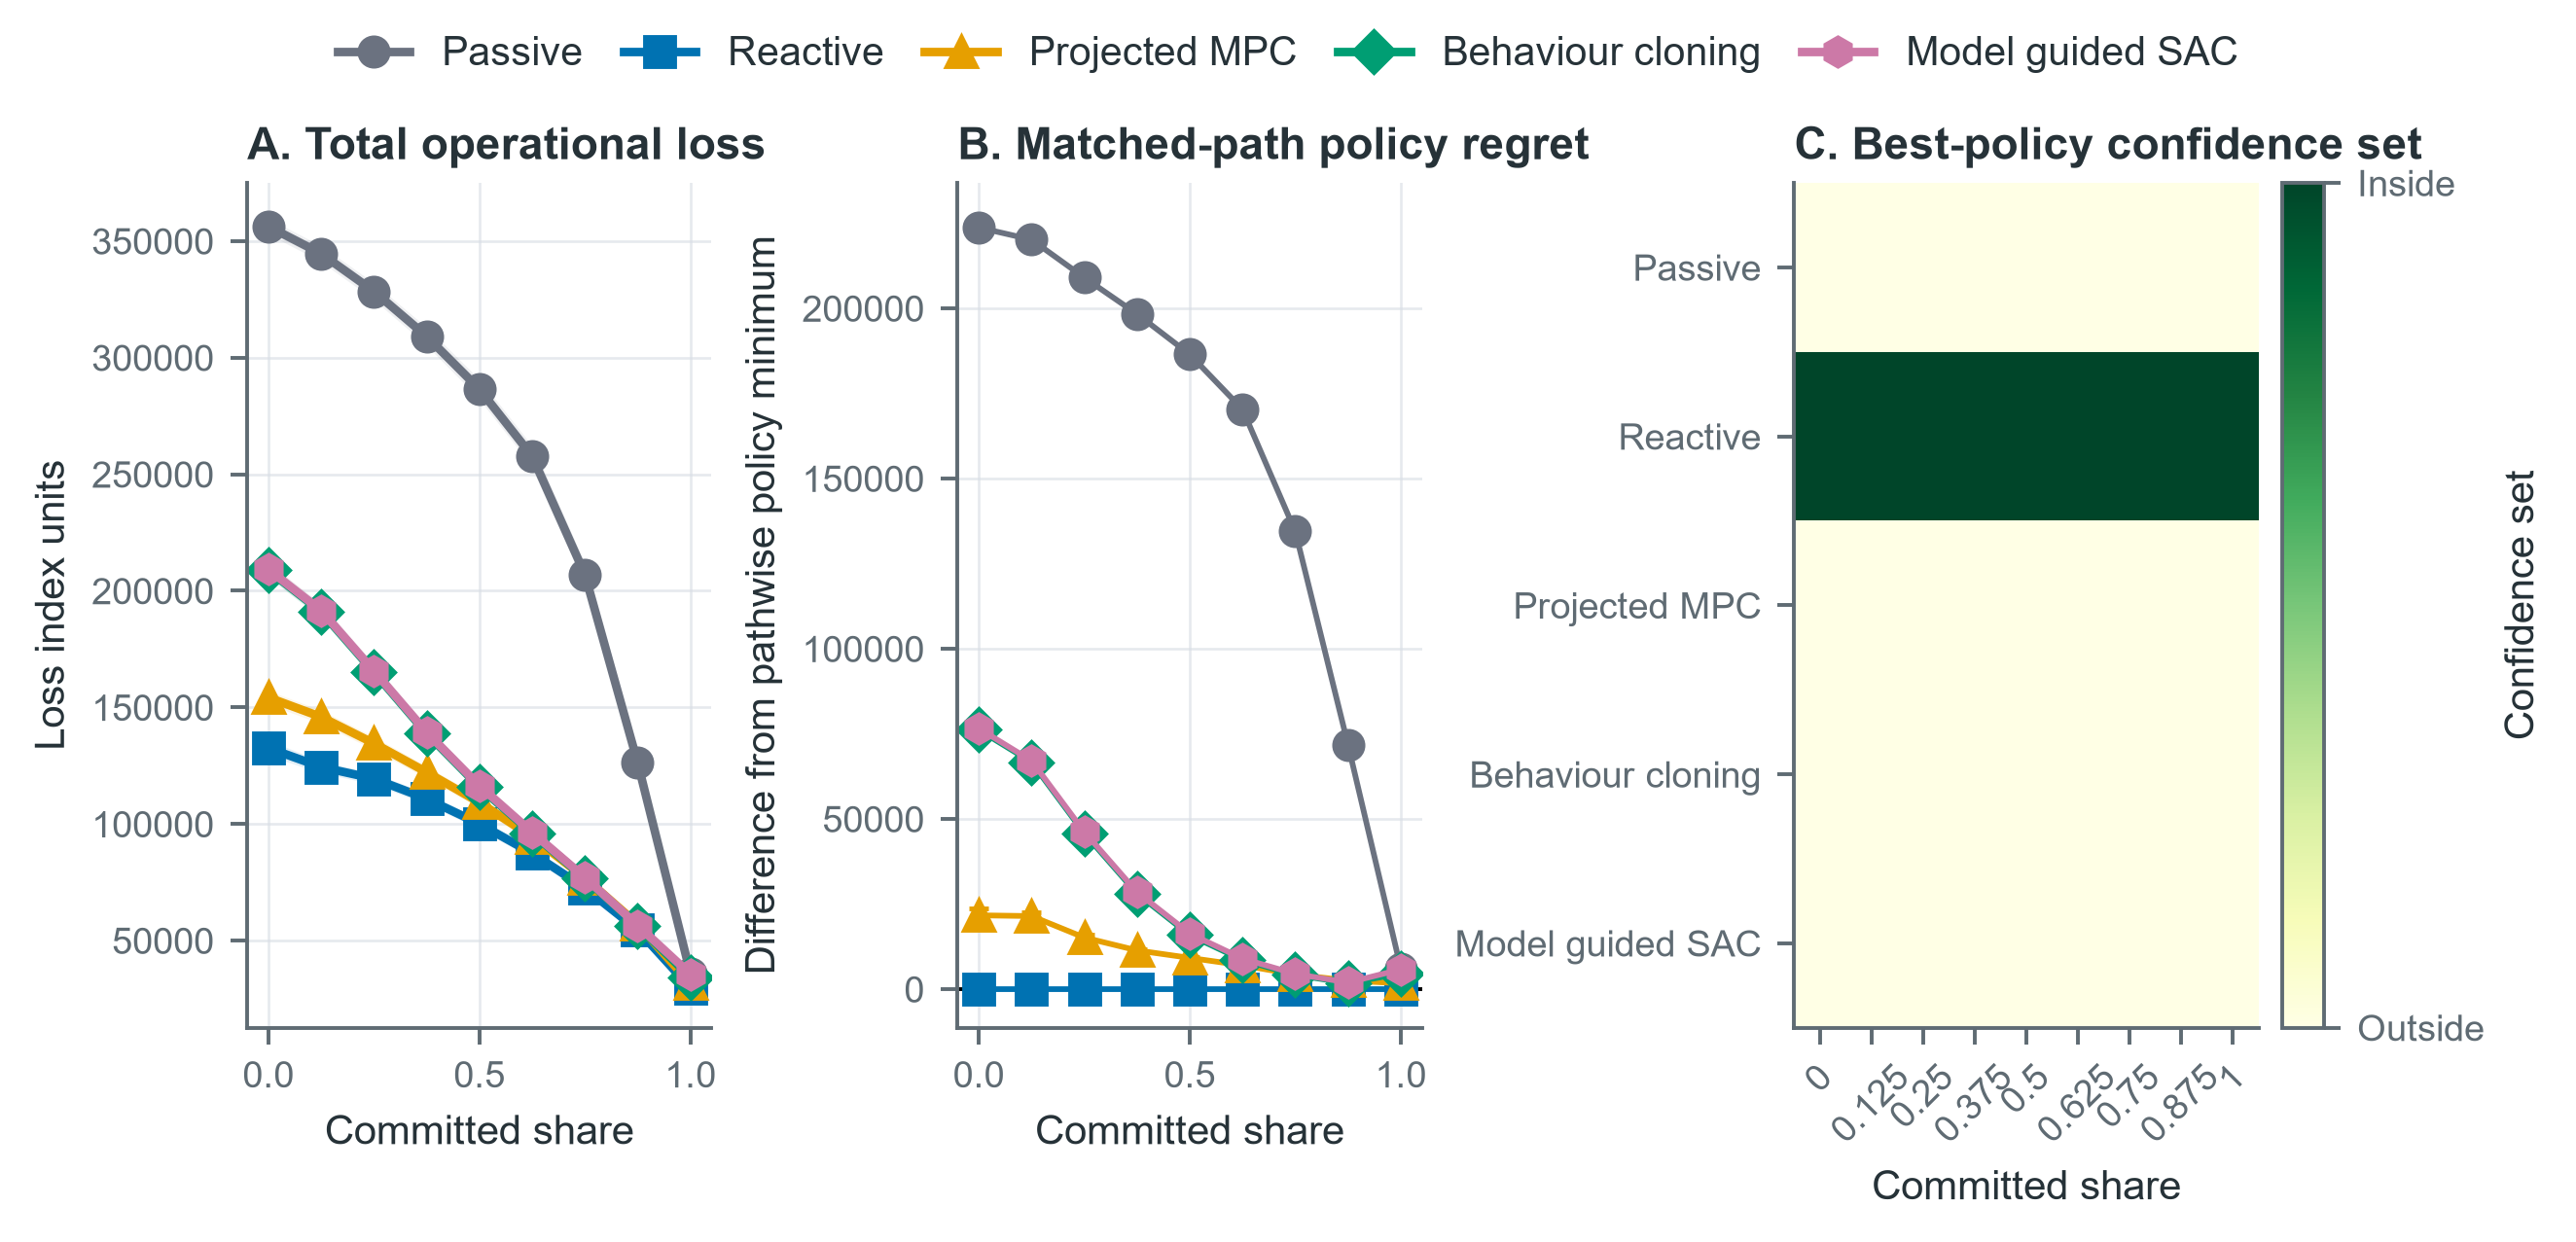
\includegraphics[width=\textwidth]{figures/figure_5_3_1a_loss_regret_confidence_set.png}
    \caption{Commitment loss and policy confidence set}
    \label{fig:531-loss-regret}
\end{figure}

Mean loss declines as $\chi$ increases for every policy, but this pattern is a
consequence of the cohort definition rather than evidence that more cargo
should be contractually locked. Figure~\ref{fig:531-wait-exit-delivery} shows
that waiting exposure, duration attrition, and adaptive delivery fall as new
blocked cargo moves into committed tagged dispatch, while committed delivery
rises. The largest mean direct SUE exit is only 0.001198 model units, so duration
attrition carries nearly all exit in these paths. All loss comparisons retain
transport, route resource, congestion, waiting, both exit channels, action, and
terminal components. For managers, the implication is diagnostic. Commitment
must be measured as a predecision constraint because it changes which mechanism
generates cost. The experiment does not support increasing commitment as an
intervention.

\begin{figure}[t]
    \centering
    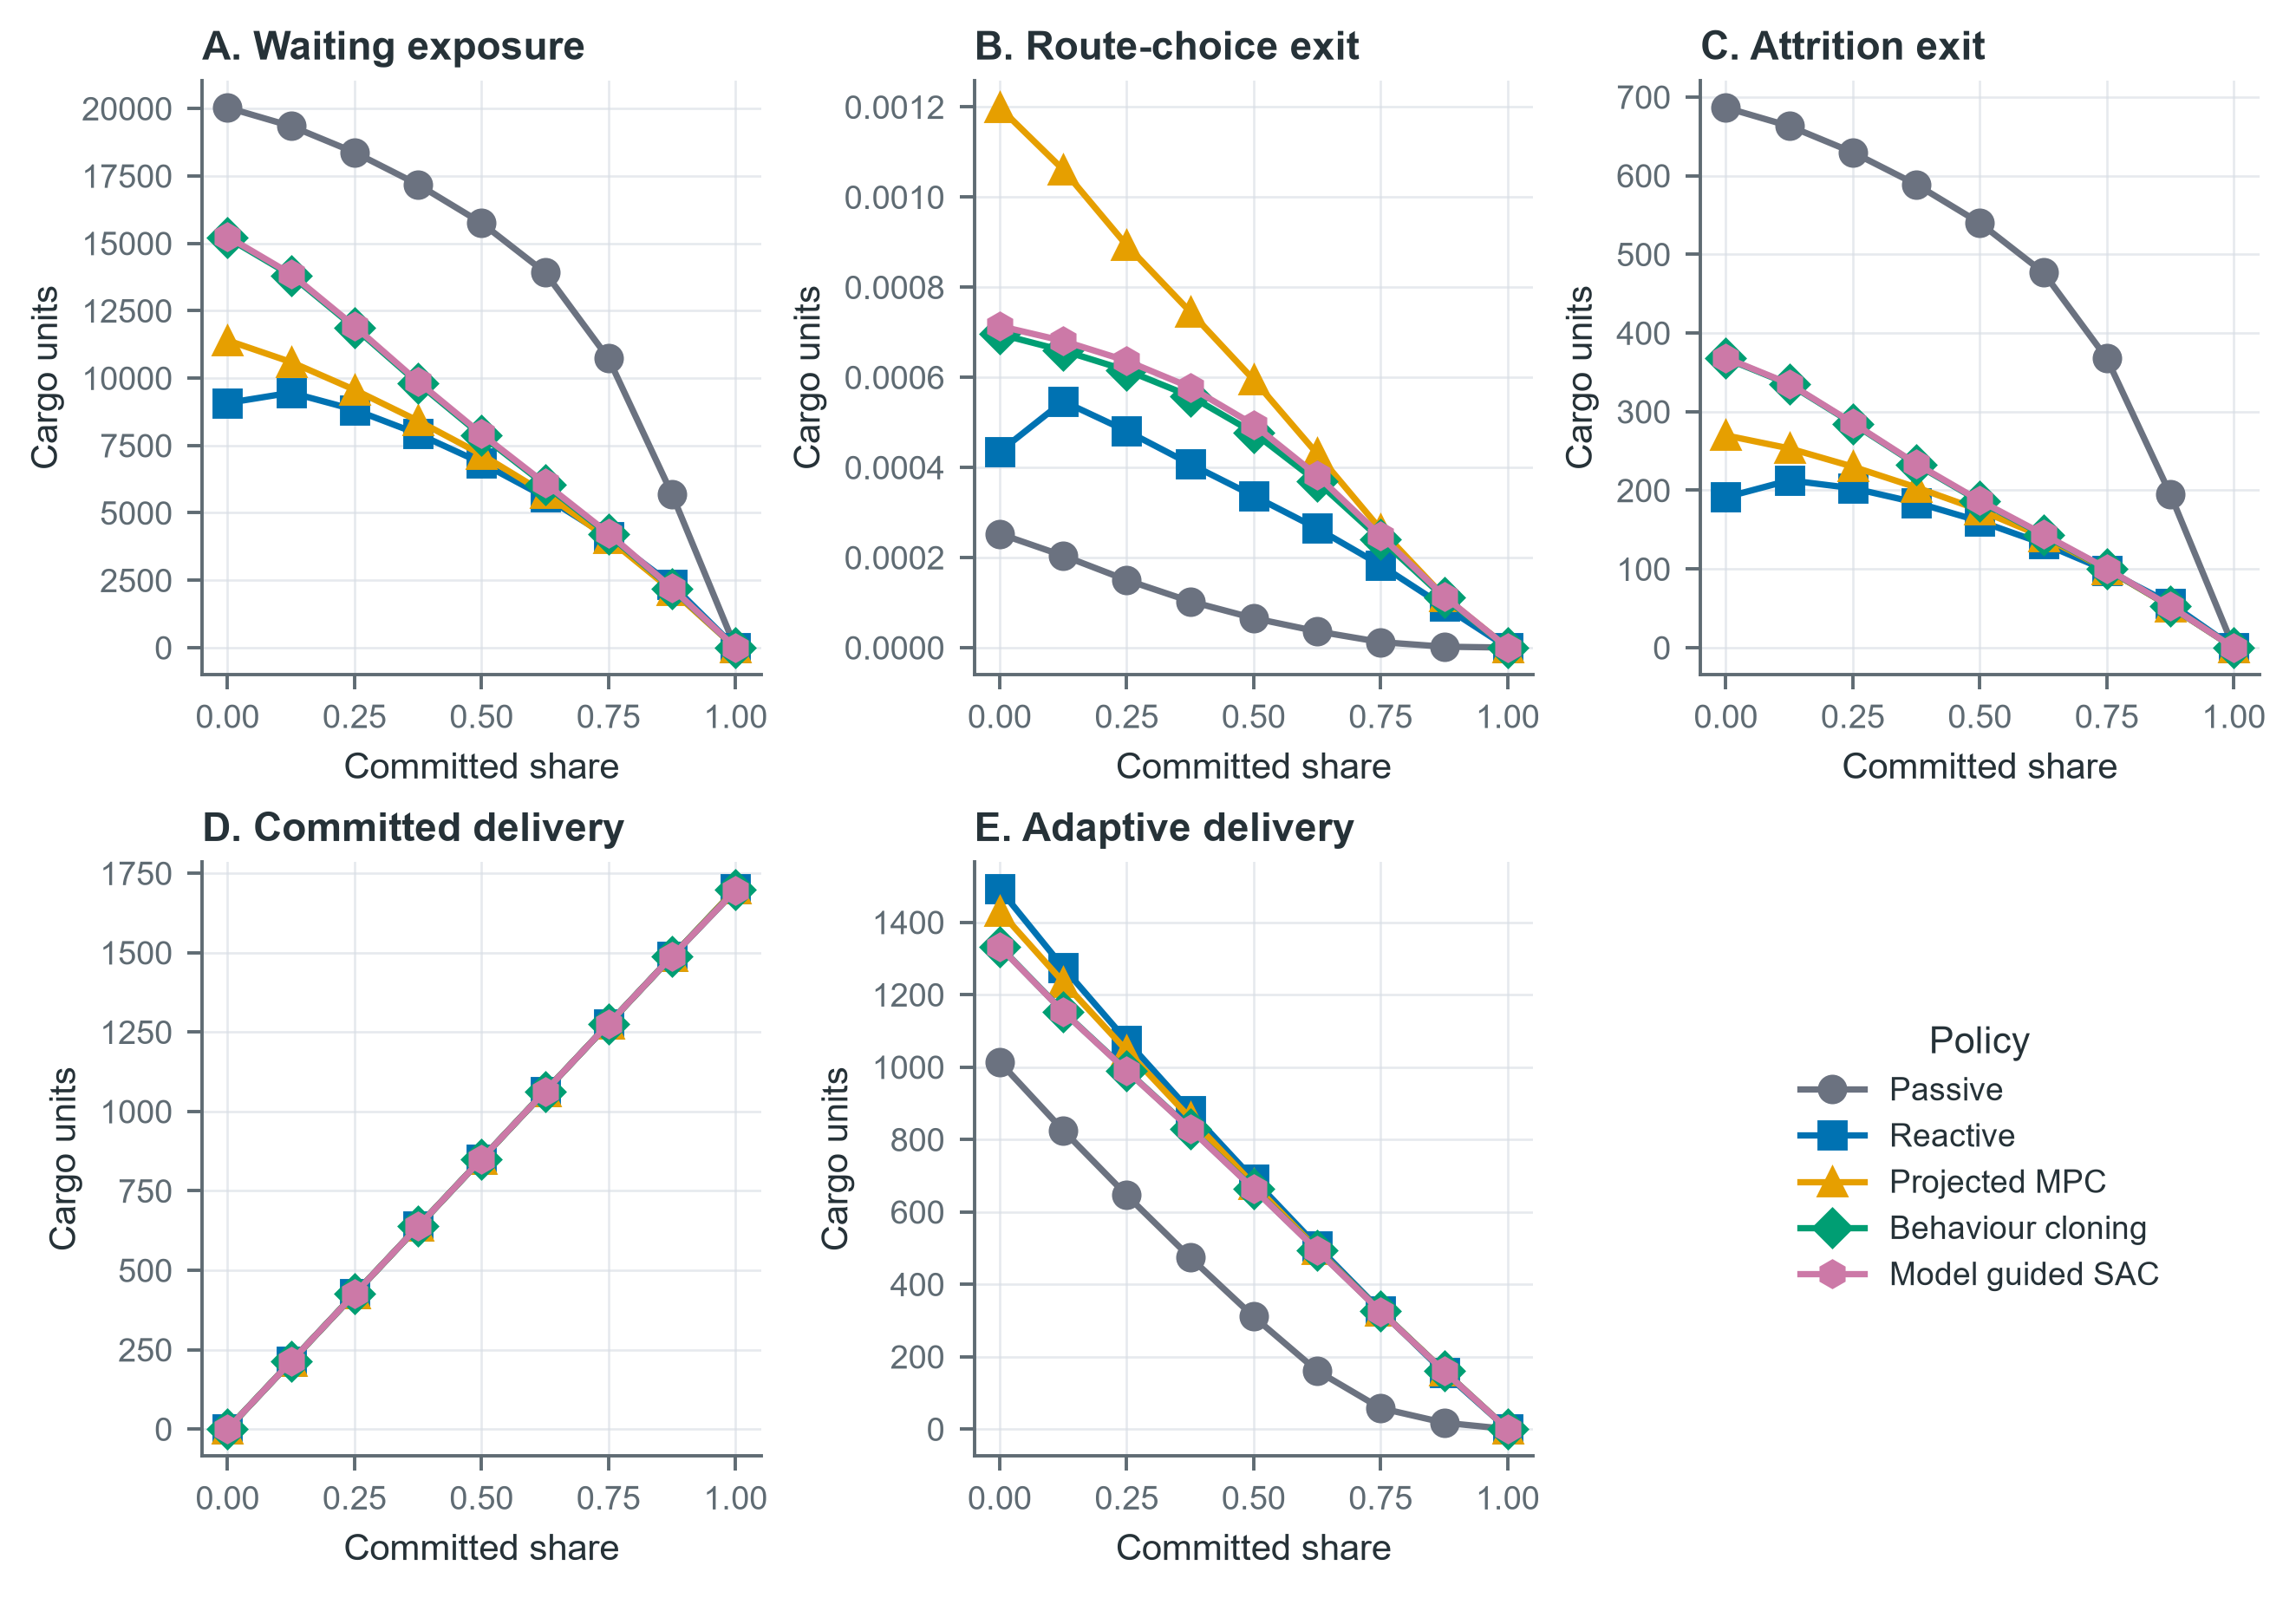
\includegraphics[width=\textwidth]{figures/figure_5_3_1b_wait_exit_delivery_mechanisms.png}
    \caption{Waiting exit and provenance delivery}
    \label{fig:531-wait-exit-delivery}
\end{figure}

Loss leadership does not imply clearance leadership. At $\chi=0$, Reactive
clears only 0.148 of the 88 paths and 75 paths are right censored, while Passive
clears every path. At $\chi=1$, clearance probabilities are 0.239 for Passive,
0.761 for Reactive, 0.795 for MPC, 0.405 for BC, and 0.288 for model guided
constrained SAC. Figure~\ref{fig:531-clearance-terminal} reports these
probabilities with restricted mean clearance time and terminal outstanding
mass. The adverse boundary result shows that lower cumulative loss can coexist
with positive terminal mass and weaker clearance. Authorities should therefore
use loss and clearance as joint decision criteria rather than infer operational
recovery from the loss ranking alone. The clearance cap classifies censoring and
does not alter actions, transitions, or losses.

\begin{figure}[t]
    \centering
    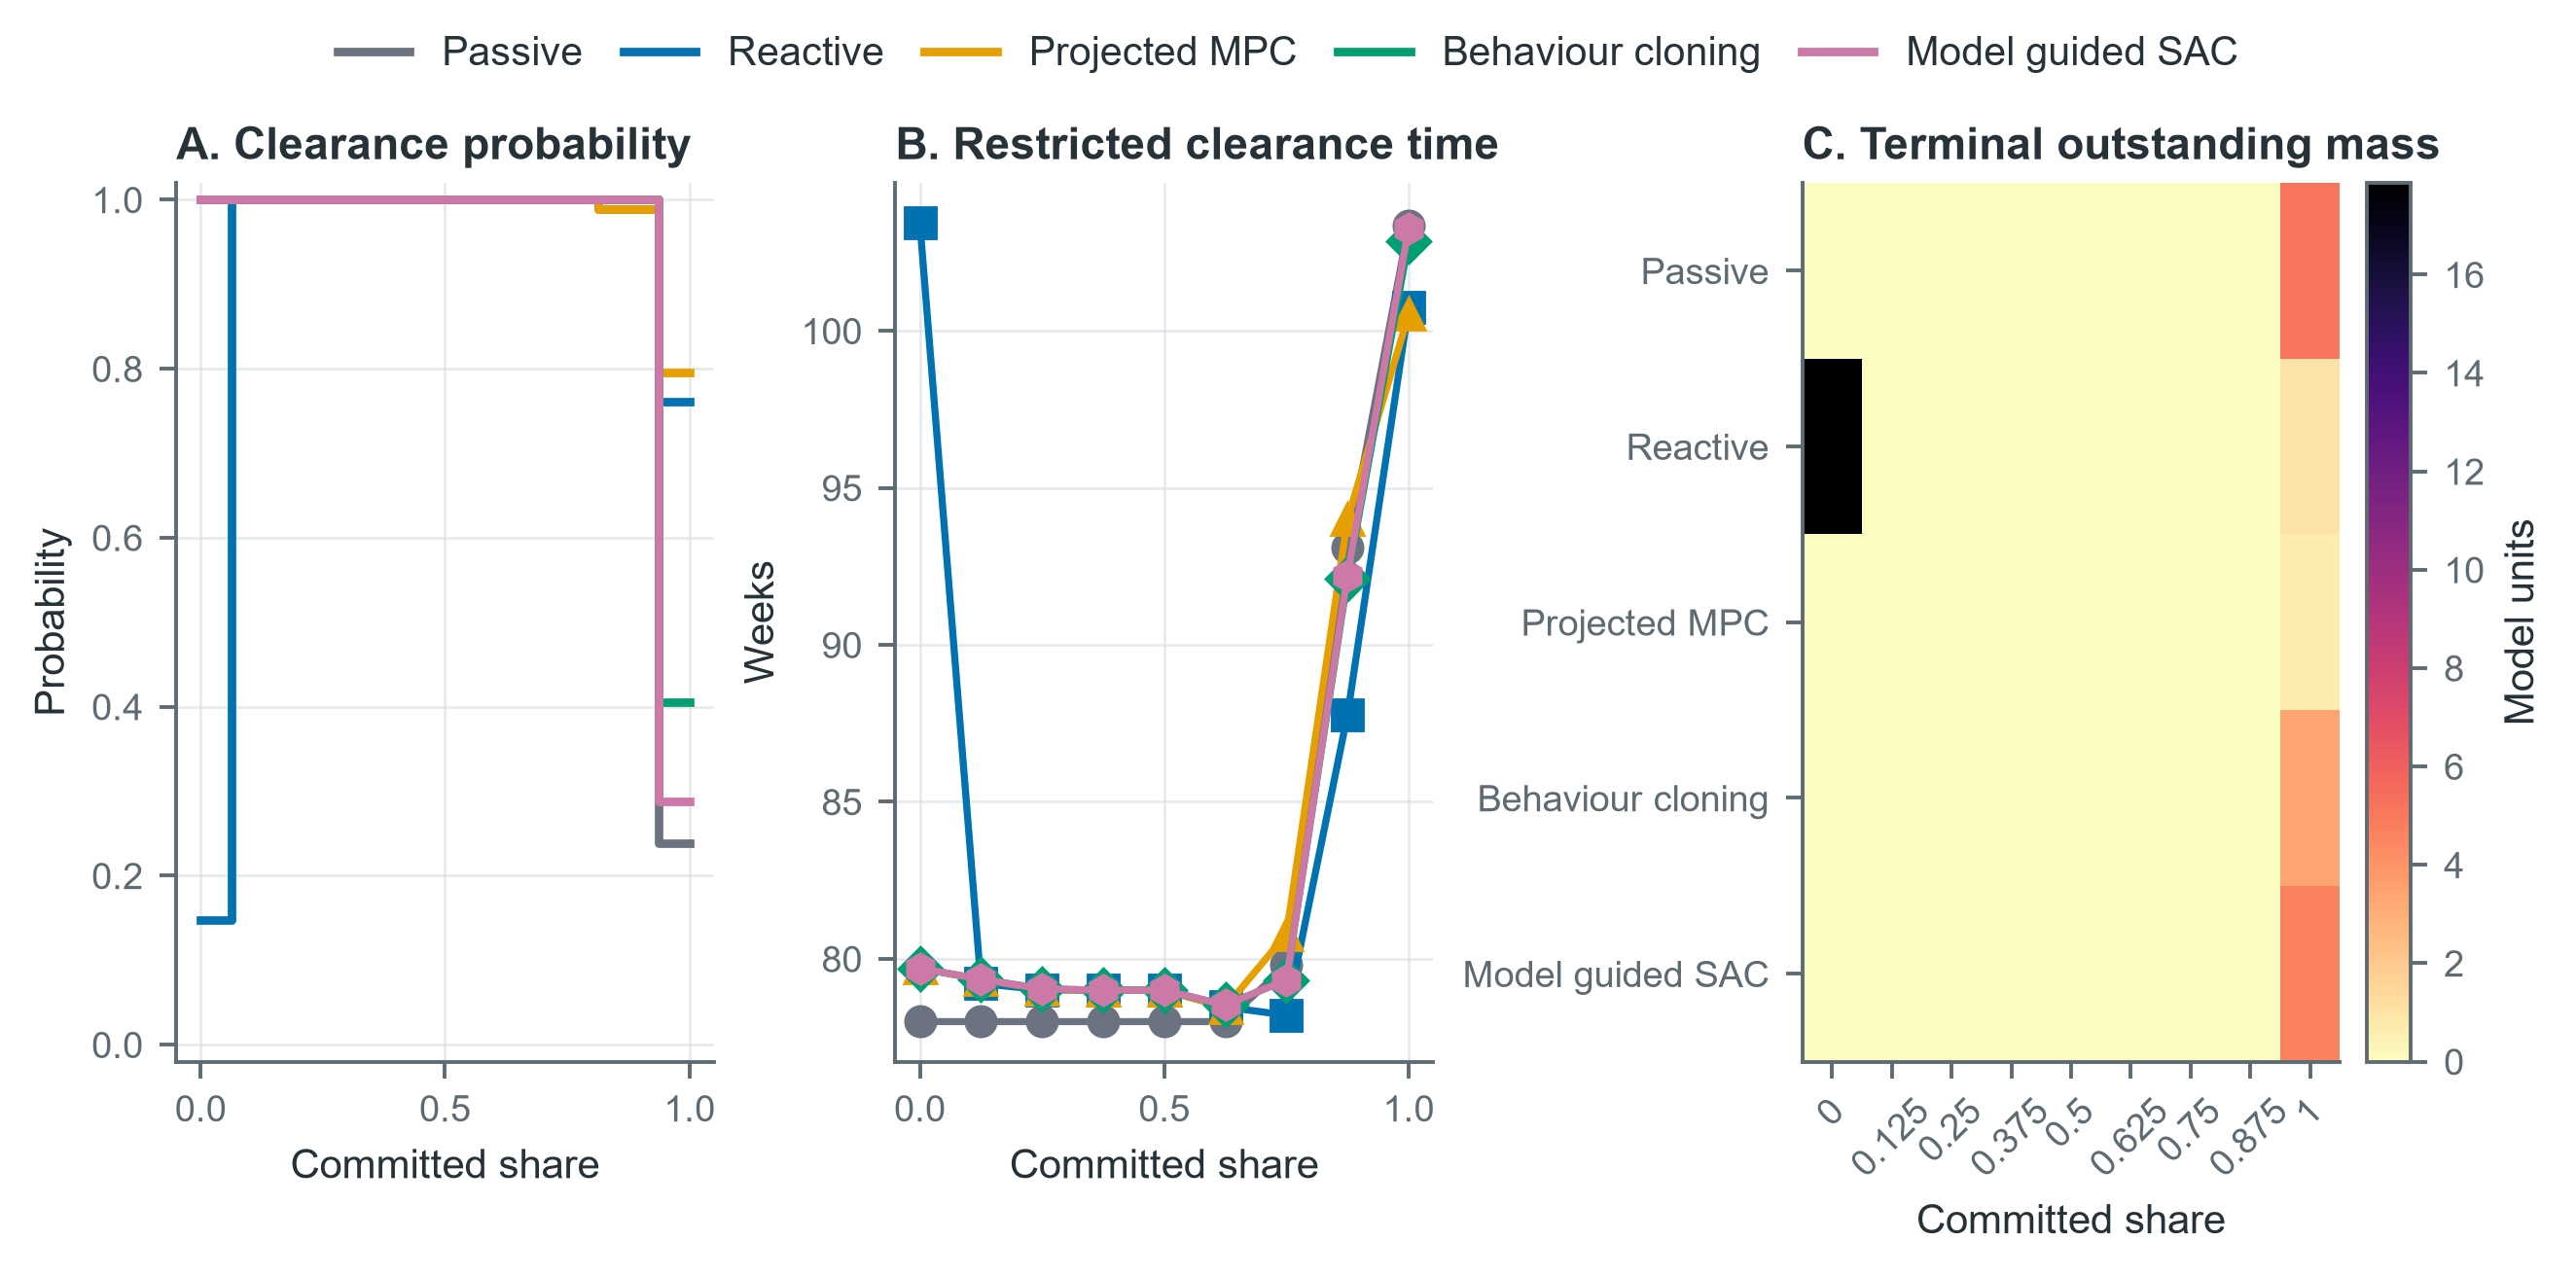
\includegraphics[width=\textwidth]{figures/figure_5_3_1c_clearance_terminal_mass.png}
    \caption{Clearance and terminal mass under commitment}
    \label{fig:531-clearance-terminal}
\end{figure}

All 16 endpoint precision targets pass. The maximum realised half width is
1,690.24 against the registered target of 2,255.64. The largest loss closure,
committed conservation, and new cohort split errors are
$3.49\times10^{-10}$, $1.67\times10^{-12}$, and
$2.13\times10^{-14}$. The maximum production transition residual is
$9.999997\times10^{-7}$ and remains within the common tolerance. The later core
contract reinforcement leaves the 7,128 trajectories, 81 checkpoints,
statistics, and figures unchanged. All 39 frozen artifact checks and 13 targeted
compatibility checks pass without retraining or full path replay.

The experimental boundary is deliberately structural. The endpoint $\chi=0$
means that no newly blocked cargo is committed. It does not remove the initial
system state. The endpoint $\chi=1$ commits every newly blocked cohort. It does
not revoke formal choices from waiting vintages that already exist. The results
therefore identify how a designed itinerary lock changes controllability under
the declared three gateway network. They do not estimate the historical Hormuz
commitment share, a field causal effect, or the value of changing commercial
contracts.

\subsubsection{Renewed Closure Sensitivity}
\label{subsubsec:reclosure-sensitivity}

The renewed closure experiment asks when the length of a temporary opening,
the intensity of a subsequent closure, and its duration change policy
performance or cross a physical recovery boundary. These quantities are
designed structural conditions rather than three observed event attributes.
The public advisories identify a 3.29 week opening and an intensity of 0.837,
but the renewed closure duration remains right censored. Table~\ref{tab:532-reclosure-inputs}
records the data and experimental roles without treating the historical marker
as a complete grid cell.

\begingroup
\setlength{\tabcolsep}{4pt}
\begin{center}
\centering
\captionof{table}{Renewed closure sensitivity inputs}
\label{tab:532-reclosure-inputs}
\begin{tabular}{>{\RaggedRight\arraybackslash}p{0.20\textwidth}
                >{\RaggedRight\arraybackslash}p{0.22\textwidth}
                >{\RaggedRight\arraybackslash}p{0.27\textwidth}
                >{\RaggedRight\arraybackslash}p{0.23\textwidth}}
\toprule
Source & Retained unit & Experimental role & Evidence boundary \\
\midrule
Accepted historical interface
& Twenty one weekly event records with the released information clock and matched residual construction
& Common event prefix, blocked flow, serviceability, and nonanticipative information
& Frozen public data supported input rather than 150 observed disruptions \\
Public event advisories
& Opening of 3.29 weeks and renewed closure intensity of 0.837
& Historical marker for opening and severity in every duration panel
& Duration remains right censored and does not select a duration cell \\
Matched physical paths
& 196 held out paths with common residual blocks and path specific continuations
& Path paired policy inference and policy independent physical certification
& Public data calibrated simulation rather than independent realised events \\
Registered deployment design
& Sixteen policy cells, three complete policy anchors, and 150 certificate cells
& Axial policy sensitivity, joint corner comparison, and complete absorption boundary
& Unevaluated policy and cell pairs receive no imputed result or ranking \\
\bottomrule
\end{tabular}
\end{center}
\endgroup

The complete grid $\mathcal G^R$, policy subset $\mathcal G^\pi$, and anchor
set $\mathcal G^A$ follow \cref{eq:reclosure-coverage-51}. At a grid point
$g=(D^{\mathrm{open}},1-a^{\mathrm{reclose}},D^{\mathrm{reclose}})$,
serviceability equals one during the opening and
$a^{\mathrm{reclose}}$ during the renewed closure. It then follows the common
recovery rule
\begin{equation}
 a^{\mathrm{rec}}_g(j)=a^{\mathrm{reclose}}_g+
 \left(1-a^{\mathrm{reclose}}_g\right)
 \frac{j}{H^{\mathrm{rec}}},
 \qquad j=1,\ldots,H^{\mathrm{rec}},
 \qquad H^{\mathrm{rec}}=8.
 \label{eq:reclosure-recovery-532}
\end{equation}
The eight week horizon equals the accepted planning and readiness horizon.
Normal activity repeats the accepted path specific residual block, and the
last legally released risk information is carried forward after the historical
prefix. The commitment share remains 0.5. Initial states, action rights,
budgets, costs, recovery, and random paths remain common. The accepted
checkpoints are deployed without grid cell retraining, which isolates the
effect of the renewed closure environment.

Policy inference is limited to the family actually evaluated at each policy
cell. For $g\in\mathcal G^\pi$, let
\begin{equation}
 \widehat\pi_g=
 \argmin_{\pi\in\Pi_g}
 \frac{1}{N^{R}_{\mathrm{path}}}
 \sum_{\omega=1}^{N^{R}_{\mathrm{path}}}
 \bar J^{\mathrm{op}}_{\pi\omega}(g),
 \qquad
 \mathcal C^{\mathrm{best}}_g=
 \left\{\pi\in\Pi_g\,\middle|\,
 L^{\mathrm{sim}}_{\pi,\widehat\pi_g}(g)\leq0\right\}.
 \label{eq:reclosure-confidence-set-532}
\end{equation}
The three learning seeds are averaged within each physical path before this
calculation. Simultaneous intervals use the three pair family for $\Pi_3$ and
the ten pair family for $\Pi_5$. The 24 precision contrasts at the three
anchors use the loss based target in \cref{eq:benchmark-path-precision}. The
required count exceeds the registered cap for the most adverse comparisons,
so all 196 matched physical paths are retained.

Renewed closure duration produces the strongest increase in operational loss,
while closure intensity also increases loss throughout the reference centred
axes, as shown in Figure~\ref{fig:532-axial-policy}. Reactive remains the sample
leader and the only retained confidence set member at every reference centred
axis cell. At nonanchor cells this statement concerns only Passive, Reactive,
and frozen BC. The widening separation from Passive reflects the accumulation
of external waiting and delayed physical absorption as closure severity and
duration increase. For a regional coordinator, the result supports early
reactive measures when a renewed closure becomes deeper or more persistent,
but it does not establish a complete five policy ranking away from the three
anchors.

\FloatBarrier
\begin{figure}[!htbp]
    \centering
    
\includegraphics[width=\textwidth,trim=0 0 0 20bp,clip]{figures/figure_5_3_2a_axial_policy_sensitivity.png}
    \caption{Axial policy sensitivity under renewed closure. Grey circles show Passive, blue squares show Reactive, and orange triangles show BC. Filled regret markers identify membership in the simultaneous confidence set}
    \label{fig:532-axial-policy}
\end{figure}
\FloatBarrier

The complete anchor comparisons reveal a conditional policy switch, as shown
in Figure~\ref{fig:532-anchor-mechanism}. At the reference anchor
$(4,0.85,8)$, Reactive has the lowest sample mean loss at 54,854.50 and is the
only member of the five policy confidence set. Under the mild corner
$(12,0.40,2)$, projected stochastic MPC becomes the sample leader at 27,797.82
and is the only retained member, compared with 34,615.53 for Reactive. All
policies clear every path at these two anchors. A long opening and brief mild
renewed closure therefore leave sufficient recovery time for anticipatory
capacity and release planning to improve the loss result without creating a
clearance tradeoff.

Under the severe corner $(1,0.95,32)$, Reactive again has the lowest sample
mean loss at 100,440.41 and is the sole confidence set member. Its clearance
probability is 0.959, whereas the four alternatives range from 0.010 to 0.155.
The experiment is conducted over the preregistered ensemble of 196 matched
physical paths. Between path variation in policy effects increases materially
at this corner. Nineteen of the 24 registered anchor contrasts attain the
target half width of 2,255.64. The remaining five contrasts are all located at
the severe corner, where the largest attained half width is 3,089.23. The
observed ordering and confidence set are retained, but estimated effect sizes
are not extrapolated beyond this evaluated ensemble. Managers should therefore
treat early reactive coordination as the most consistently supported response
within the declared severe scenarios rather than as a universally optimal
controller.

\FloatBarrier
\begin{figure}[!htbp]
    \centering
    
\includegraphics[width=\textwidth]{figures/figure_5_3_2b_anchor_mechanism_recovery.png}
    \caption{Anchor mechanisms and recovery under renewed closure}
    \label{fig:532-anchor-mechanism}
\end{figure}
\FloatBarrier

The recovery results also prevent a loss ranking from being mistaken for a
clearing time ranking. Across the evaluated policy cells, 808 path policy
summaries remain right censored. These observations enter clearance probability
and restricted mean clearance time, and none is assigned the 104 week cap as an
observed clearing time. This distinction is operationally material because a
controller can reduce cumulative queue and waiting loss while leaving positive
terminal mass under an adverse physical path. Authorities should therefore
monitor loss, clearance probability, restricted mean clearance time, and final
outstanding mass jointly.

The policy independent certificate identifies a broad physical boundary, as
reported in Figure~\ref{fig:532-absorption}. All 196 matched paths violate the
optimistic absorption condition in 118 of the 150 structural cells, and at
least one path violates it in 137 cells. A violation proves that threshold
crossing cannot be avoided even after removing future arrivals, relaxing
budget coupling, applying the optimistic component capacity envelope, and
assigning shared corridor capacity favourably. In these regimes managers need
to prioritise demand containment, emergency capacity, and corridor recovery
because fine differences in controller loss cannot restore physical
absorbability.

\FloatBarrier
\begin{figure}[!htbp]
    \centering
    
\includegraphics[width=\textwidth]{figures/figure_5_3_2c_full_absorption_certificate.png}
    \caption{Optimistic absorption boundary under renewed closure. Squares identify the 16 policy cells, stars identify the three complete policy anchors, and hatching identifies cells where all matched paths violate the certificate. The historical opening and intensity marker appears in every duration panel because duration remains right censored}
    \label{fig:532-absorption}
\end{figure}
\FloatBarrier

Certificate nonviolation has no converse interpretation. An unhatched cell may
still fail under the dynamic equilibrium, action budget, shared corridor, or
finite clearance horizon. The historical opening and intensity marker appears
in every duration panel because duration is unobserved rather than because the
event belongs to every duration cell. The experiment therefore supports axial
deployment sensitivity, two joint corners, and a complete physical
impossibility boundary. It does not support a five policy ordering across all
150 cells, a complete three factor policy interaction surface, guaranteed
feasibility in certificate nonviolating cells, or a field causal effect.

\subsubsection{Gateway Network Sensitivity}
\label{subsubsec:gateway-network-sensitivity}

The gateway network experiment asks whether a larger portfolio creates usable
diversification or merely redistributes congestion across a fixed regional
chain. A gateway denotes a complete route tagged itinerary through maritime
transport, berth, yard, gate, and the shared landbridge corridor. The
experiment therefore concerns regional gateway architecture rather than port
count alone. The observed three gateway network is compared with semi
synthetic portfolios of four, five, seven, and nine gateways. Every added node
inherits the median stage capacity, maritime lag, and waiting error scale of
the three observed gateways. No added node is interpreted as a forecast for a
named port.

The 25 declared cells follow \cref{eq:gateway-network-design-51}. Capacity
neutral designs increase the number of route alternatives while retaining the
observed aggregate gateway capacity and shared corridor. Port only designs add
gateway stage capacity while leaving the shared corridor fixed. End to end
designs add both gateway stages and their corridor contribution. Emergency
only additions serve adaptive cargo, whereas precontracted additions also
enter the committed itinerary set. Each cell uses the same 23 matched physical
paths. Learning seeds are first averaged within path. A new teacher, BC
controller, and constrained SAC controller are produced for every network
size because the formal action dimension increases from 34 to 94. Size
specific controllers are then held fixed across architecture and eligibility
conditions. Passive, Reactive, and BC are evaluated in all cells. Projected
stochastic MPC and model guided constrained SAC are additionally evaluated at
the observed reference and the six nine gateway endpoints. Unevaluated policy
and cell pairs receive no imputed loss or ranking.

Figure~\ref{fig:533-loss-regret} shows that gateway expansion changes both
system loss and the relative value of policy computation. In the observed
three gateway reference, mean operational loss is 99,362.09 for Reactive,
108,668.67 for projected stochastic MPC, 115,949.64 for BC, 116,409.19 for
model guided constrained SAC, and 288,769.30 for Passive. Reactive is the
sample leader in 14 of the 25 evaluated cells. BC leads the three policy family
in five intermediate network cells. When all five policies are compared at
the six nine gateway endpoints, projected stochastic MPC is the sample leader
in every case. The change does not establish one universally best controller.
It shows that a larger route and action space increases the value of solving
the network specific coordination problem rather than transferring the
reference policy ordering without revaluation.

\begin{figure}[t]
    \centering
    
\includegraphics[width=\textwidth]{figures/figure_5_3_3a_loss_regret_network.png}
    \caption{Gateway network loss and policy regret}
    \label{fig:533-loss-regret}
\end{figure}

The matched architecture contrasts show why gateway count alone is
insufficient. Under Reactive and emergency only access, moving from three
observed gateways to nine capacity neutral gateways lowers mean loss by
20,868.06 units. With precontracted access the corresponding reduction is
35,962.08. This is diversification value because total declared capacity is
held fixed. Adding port side capacity to the nine gateway emergency network
reduces Reactive loss by a further 9,160.81. The same port only change under
precontracting instead increases loss by 2,720.19, which reveals a loading and
bottleneck interaction rather than an unconditional capacity benefit. Adding
the corridor contribution after port expansion lowers Reactive loss by 441.38
under emergency access and 775.94 under precontracting. Precontracting itself
lowers Reactive loss by 15,094.02 in the capacity neutral architecture,
3,213.02 in the port only architecture, and 3,547.58 in the end to end
architecture. Thus contractual eligibility can create more usable value than
an isolated increase in physical capacity.

Figure~\ref{fig:533-overload} holds the Reactive policy fixed and identifies
where the burden moves. The fraction of gateways experiencing overload falls
as the portfolio expands, but total resource week overload need not fall. In
the nine gateway capacity neutral emergency design, overloaded gateway
incidence falls from 0.667 to 0.222 while resource week overload rises from
194.35 to 363.04. The additional alternatives spread exposure across more
locations without increasing the aggregate service envelope. Port only
expansion reduces gateway overload but creates positive shared corridor
overload. End to end expansion removes this corridor exposure. Under the nine
gateway precontracted design, end to end expansion yields resource week
overload of 52.74 and overloaded gateway incidence of 0.111. A coordinator
should therefore monitor both overload incidence and total overload duration.
A lower affected share is not evidence that the regional burden has fallen.

\begin{figure}[t]
    \centering
    
\includegraphics[width=\textwidth]{figures/figure_5_3_3b_network_overload.png}
    \caption{Gateway and corridor overload under network expansion}
    \label{fig:533-overload}
\end{figure}

The flow outcomes in Figure~\ref{fig:533-flow-clearance} reinforce this
distinction. Under Reactive, every nine gateway architecture lowers waiting
exposure and increases delivered cargo relative to the observed reference.
However, the capacity neutral emergency design does not clear within the
declared horizon on any matched path and retains mean terminal mass of 27.81.
Precontracting restores clearance in the matched ensemble and raises delivered
cargo from 1,593.02 to 1,608.77. Both port only and end to end nine gateway
designs clear under the evaluated access conditions, although their overload
locations differ. A low cumulative loss or low gateway incidence must
therefore be read jointly with clearance and terminal mass.

\begin{figure}[t]
    \centering
    
\includegraphics[width=\textwidth]{figures/figure_5_3_3c_flow_clearance.png}
    \caption{Waiting delivery and clearance under gateway expansion}
    \label{fig:533-flow-clearance}
\end{figure}

The managerial conclusion is that an alternative gateway has value only when
four conditions align. It must provide an additional route choice, possess
usable port side service, connect to sufficient shared corridor capacity, and
be contractually available to the relevant cargo cohort. Capacity neutral
expansion identifies diversification value. Port only expansion can transfer
the bottleneck inland. End to end expansion closes the physical chain, while
precontracting closes the eligibility gap. These are conditional structural
findings for the declared event, costs, policies, and semi synthetic network
templates. They do not estimate the effect of constructing a particular port
or guarantee that a larger gateway portfolio will improve every policy and
physical path.

\FloatBarrier

\subsubsection{Parameter Robustness}
\label{subsubsec:parameter-robustness}

The parameter robustness experiment asks whether the benchmark policy ordering
and its congestion mechanisms persist when publicly unidentified behavioural,
physical, economic, control, and information inputs move away from their
reference values. It uses one factor screening and four declared combined
stresses rather than a high dimensional factorial design. The levels in
\cref{eq:robustness-transformations-51,eq:robustness-design-51} are designed
structural conditions and not estimated confidence intervals. Commitment
remains fixed at $\chi=0.5$ because its complete admissible domain is evaluated
in the commitment experiment.

Table~\ref{tab:534-robustness-inputs} records the evidence used in this
experiment. No new historical observation is introduced. The accepted event
interface, reference parameter register, matched path constructor, severe
renewed closure endpoint, and semi synthetic gateway constructor retain their
previous evidence status.

\begingroup
\setlength{\tabcolsep}{4pt}
\begin{table}[t]
\centering
\caption{Parameter robustness inputs}
\label{tab:534-robustness-inputs}
\begin{tabular}{>{\RaggedRight\arraybackslash}p{0.20\textwidth}
                >{\RaggedRight\arraybackslash}p{0.22\textwidth}
                >{\RaggedRight\arraybackslash}p{0.27\textwidth}
                >{\RaggedRight\arraybackslash}p{0.23\textwidth}}
\toprule
Source & Retained unit & Experimental role & Evidence boundary \\
\midrule
Accepted historical interface
& Twenty one weekly event records with released risk states and event inputs
& Common event clock, serviceability, blocked flow, and nonanticipative information
& Frozen public data supported input rather than a new disruption sample \\
Reference parameter register
& Thirteen behavioural, physical, economic, control, and information factors
& Common reference and two declared nonreference endpoints for each factor
& Reference centred structural levels rather than estimated parameter intervals \\
Matched physical paths
& Ten held out paths selected by the outcome blind eight hour timing rule
& Path paired effects, policy regret, confidence sets, clearance, and mechanism outcomes
& Conditional simulation ensemble rather than independent realised events \\
Policy and structural registers
& Accepted reference checkpoints, matched severe closure training, a size matched nine gateway checkpoint, and four combined stresses
& Controller support, checkpoint selection, structural constructors, and replay acceptance
& Unevaluated policies are retained as not run and receive no imputed result \\
\bottomrule
\end{tabular}
\end{table}
\endgroup

The 31 simulated cells contain the common reference, two nonreference levels
for each of 13 one factor screens, and four combined structural stresses. The
combined stresses pair a doubled maritime lag with the one week opening, 0.95
renewed closure intensity, and 32 week renewed closure endpoint, the reference
convex waiting hazard with half exit consequence, the nine gateway end to end
precontracted network with half shared corridor capacity, and a sixteen week
readiness lead with the design midpoint $\gamma_I=0.5$. The first combination
uses the common eight week recovery. The second is algebraically identical to
the half exit consequence main effect because $p=2$ is the reference waiting
hazard. It is therefore an identity audited combined anchor rather than an
identified nonadditive interaction.

Policy coverage follows the state and action dimensions supported in each
cell. Passive, Reactive, and BC are evaluated in 22 dimension compatible one
factor cells. The two maritime lag cells, two readiness lead cells, and the
long readiness and low credibility combination compare Passive, Reactive, and
online MPC because their model input dimension changes. The common reference
and the other three combined anchors compare all five declared policies. BC
and full constrained SAC are retrained only for the long lag and severe closure
anchor. The nine gateway anchor uses the size matched checkpoint that was
frozen before the corridor stress. No lower dimensional checkpoint is padded,
and no missing policy is interpolated.

For a cell $c$, policy $\pi$ evaluated at both $c$ and the common reference,
and physical path $\omega$, define the paired deployment effect and within cell
regret as
\begin{equation}
 \Delta^P_{c,\pi,\omega}
 =\bar J^{\mathrm{op}}_{c,\pi,\omega}
 -\bar J^{\mathrm{op}}_{\mathrm{ref},\pi,\omega},
 \qquad
 R^P_{c,\pi,\omega}
 =\bar J^{\mathrm{op}}_{c,\pi,\omega}
 -\min_{\pi'\in\Pi_c}
 \bar J^{\mathrm{op}}_{c,\pi',\omega}.
 \label{eq:parameter-robustness-effects}
\end{equation}
The three learning seeds are averaged within each path before either quantity
is calculated. Simultaneous intervals and Holm adjusted tests are formed within
each declared family. The best policy confidence set is
\begin{equation}
 \widehat\pi_c=
 \argmin_{\pi\in\Pi_c}\frac{1}{N^P_{\mathrm{path}}}
 \sum_{\omega}\bar J^{\mathrm{op}}_{c,\pi,\omega},
 \qquad
 \mathcal C^{\mathrm{best}}_c=
 \left\{\pi\in\Pi_c\,\middle|\,
 L^{\mathrm{sim}}_{c,\pi,\widehat\pi_c}\leq0\right\},
 \qquad N^P_{\mathrm{path}}=10.
 \label{eq:parameter-robustness-confidence-set}
\end{equation}
The timing rule fixes the ten paths before test outcomes are read. All
inference is therefore conditional on this matched physical path ensemble and
the policy family $\Pi_c$ actually evaluated in each cell.

Figure~\ref{fig:534-parameter-effects} shows the Reactive cell minus reference
effects. Doubling network exposure produces the largest loss increase at
188,662.22, with a simultaneous interval from 179,804.93 to 197,519.52. The
long lag and severe renewed closure combination increases loss by 122,609.08,
with an interval from 86,132.86 to 159,085.29. Doubling maritime lag and halving
port service increase loss by 78,500.95 and 37,516.43. These effects locate the
largest deployment risks in demand scale, travel time, and physical service.
The maritime lag stress also retains its registered lag based real resource
increment, while port service and corridor stresses preserve the corresponding
one service week congestion thresholds. They are therefore coherent system
stresses rather than isolated coefficient changes.

The largest Reactive loss reduction occurs under the concave waiting hazard
$p=0.5$ at 76,472.20 units. This change arises because earlier waiting vintages
receive a larger attrition hazard and is not a recommendation to accelerate
cargo exit. The authority budget endpoints produce zero loss change for the
frozen Reactive rule, which means that the registered budget is nonbinding on
these ten paths. A four week readiness lead produces a change of $-154.94$
with an interval from $-379.67$ to 69.79. Neither result establishes that
budget or preparation time is generally immaterial.

\begin{figure}[t]
    \centering
    
\includegraphics[width=\textwidth]{figures/figure_5_3_4a_parameter_effect_forest.png}
    \caption{Reactive parameter and combined stress effects}
    \label{fig:534-parameter-effects}
\end{figure}

Policy identity is stable across most declared comparisons but has two
material structural exceptions. Figure~\ref{fig:534-policy-stability} shows
that 30 of the 31 cells have one member in the simultaneous confidence set
within their evaluated policy family. On the ten path common reference,
Reactive loss is 98,871.13 and it is the sole confidence set member. The
corresponding losses are 108,011.97 for MPC, 114,230.87 for BC, 114,762.68 for
model guided constrained SAC, and 286,265.04 for Passive. These are conditional
deployment anchors for the robustness ensemble and do not replace the complete
benchmark estimates. Reactive is the sample leader in 28 cells and belongs to
the confidence set in 29 cells. At half maritime lag, MPC
has a sample advantage of only 21.12 over Reactive and its interval from
$-880.80$ to 923.04 retains both policies. At doubled maritime lag, MPC leads
Reactive by 9,415.47, with an interval from 4,231.90 to 14,599.03. In the nine
gateway and low corridor combined stress, MPC leads Reactive by 33,668.74,
with an interval from 32,982.72 to 34,354.76. A coordinator should therefore
reconsider an online planning policy when maritime timing or network dimension
departs substantially from the reference, but these cells do not establish a
general MPC advantage under every stronger stress.

BC enters none of the confidence sets in its 26 evaluated cells. Model guided
constrained SAC enters none of the four complete policy anchor sets. At the
matched long lag and severe closure anchor, BC and model guided constrained SAC
remain 41,828.98 and 43,580.88 above Reactive after matched training. This
negative result shows that matched support does not close their performance
gap at that endpoint. Model guided constrained SAC is not evaluated in the
behavioural and economic one factor screens, so those cells do not establish
its parameter robustness. White entries in
Figure~\ref{fig:534-policy-stability} denote policies not evaluated by design
and not policy failures.

\begin{figure}[t]
    \centering
    
\includegraphics[width=\textwidth]{figures/figure_5_3_4b_policy_stability.png}
    \caption{Policy confidence set stability}
    \label{fig:534-policy-stability}
\end{figure}

The mechanism outcomes in Figure~\ref{fig:534-interaction-mechanisms} explain
why the combined stresses cannot be reduced to a common severity scale. Under
long lag and severe renewed closure, Reactive loss is 221,480.21, clearance
probability is 0.70, and mean terminal outstanding mass is 4.962. BC, MPC, and
model guided constrained SAC each clear 0.30 of their paths. Reactive remains
the sole confidence set member, but the pressure is expressed mainly through
port stage overload, waiting, and terminal mass rather than shared corridor
overload alone. A small corridor measure is therefore not evidence that the
network has no bottleneck.

The convex hazard and low exit anchor reduces Reactive loss by 2,337.51 while
direct SUE exit rises from approximately zero to 11.837 model units. Because
this anchor reproduces the half exit consequence main effect, it verifies the
registered identity but does not identify an independent interaction. In the
nine gateway and half corridor combination, all evaluated policies clear and
MPC loss is 32,093.06 compared with 65,761.80 for Reactive. This cell changes
both the network and corridor condition. Its lower loss relative to the three
gateway reference cannot be attributed to reducing corridor capacity. The
network architecture comparisons remain the evidence for that separate
component effect.

The sixteen week readiness and low credibility combination increases Reactive
loss by 204.82, with an interval from 39.35 to 370.29, and leaves Reactive as
the sole confidence set member. It measures the total policy response to this
combined condition. It does not recompute $V_{R\mid D}$, $V_{D\mid R}$, or
$S_{RD}$ and therefore does not reidentify whether readiness and direct
procurement are complements or substitutes. The conditional capacity right
estimands in Figure~\ref{fig:524-capacity-portfolio} remain the evidence for
that relationship.

\begin{figure}[t]
    \centering
    
\includegraphics[width=\textwidth]{figures/figure_5_3_4c_interaction_mechanisms.png}
    \caption{Mechanisms under combined structural stresses}
    \label{fig:534-interaction-mechanisms}
\end{figure}

Clearance and failure diagnostics provide an additional boundary. When network
exposure is doubled, Passive, Reactive, and BC clear none of the matched paths.
When port service is halved, Reactive clears 0.10 and the other two policies
clear none. Across the 1,010 evaluated path policy summaries, 91 are right
censored and no numerical failure occurs. At the common reference, terminal
mass lies between $5.52\times10^{-7}$ and $7.12\times10^{-7}$. Reclassifying
these same terminal states at $10^{-8}$ marks every policy as uncleared, while
$10^{-6}$ and $10^{-4}$ mark every policy as cleared. The diagnostic changes no
action, transition, loss, or terminal state and is not a reoptimised clearance
experiment.

The 1,610 policy path seed runs satisfy the registered trajectory and numerical
contracts. The maximum transition residual is $9.99985\times10^{-7}$ and the
maximum loss closure error is $4.66\times10^{-10}$. These checks establish
internal acceptance rather than field effectiveness. The substantive evidence
is conditional on the ten paths chosen by the prespecified computational rule,
the policy family supported in each cell, the declared reference centred
levels, and the four combined anchors. It does not provide a high dimensional
uncertainty distribution, an empirical parameter confidence region, a causal
field effect, or a universal controller ranking.

\FloatBarrier
\section{Discussion and Conclusions}
\label{sec:discussion-conclusions}

The analysis answers RQ1 by showing that congestion propagation is governed by
the interaction of four cargo responses and two feedback channels. Gateway
commitment fixes part of the spatial burden before a coordinator acts. The
route-and-waiting equilibrium determines whether the remaining cargo enters a
gateway or stays outside. Tagged queues then transmit arrivals through berth,
yard, gate, and landbridge stages, while downstream congestion changes upstream
service and later route costs. The same observed transit loss can therefore
produce different queue, waiting, and clearance outcomes without violating mass
conservation.

The answer to RQ2 is conditional rather than an algorithm ranking by novelty.
Model guidance is useful because stochastic MPC teacher data give the actor a
structured initialization and because behavior cloning executes about 56 times
faster than online MPC. Constrained SAC refinement passes the implementation and
activation audit, and the model-guided selector wins validation for two of three
seeds. It nevertheless increases historical mean loss from 5567.26 under
behavior cloning to 5643.31 and more than doubles external waiting. Stochastic
MPC remains the historical loss leader, while reactive coordination leads both
stress tests. The results reject the proposition that DRL is operationally
superior merely because it is newer. In a small and highly structured gateway
system, a strong teacher or state-triggered rule can remain preferable. Learning
becomes most defensible when online latency, a larger action space, or repeated
deployment makes MPC rollouts costly, but that scalability claim requires a
separate network-size experiment.

The reclosure map sharpens this conditional answer. Reactive coordination is the
appropriate default across most of the tested region because its observable
state trigger captures the main congestion mechanism at negligible online
cost. Scenario based MPC becomes preferable only when renewed closure is both
severe and persistent and when the temporary reopening is too short to drain
the committed wave. Once the optimistic absorption boundary is crossed, the
priority changes again. The decision is no longer which controller removes all
overload, but how to reserve physical capacity, limit new commitments, and
manage waiting and exit transparently. This creates an operational policy switch
rule without claiming that a more complex algorithm dominates every state.

Three managerial implications follow. First, coordinators should measure
gateway commitment before issuing diversion guidance. When the committed wave
approaches optimistic absorption capacity, information cannot prevent every
threshold crossing and scarce physical capacity should be reserved for the most
consequential stages. Second, external waiting must appear on the operating
dashboard. A policy that lowers port overload by holding cargo outside can still
raise delay and inventory exposure. Third, risk monitoring should be tied to a
specific reversible readiness instrument. A filtered geopolitical state without
a forecast horizon, publication lag, procurement lead time, expiry rule, and
false-warning cost is not an operational early-warning system.

The study also has clear limitations. PortWatch measures AIS-derived activity
proxies and may be revised. The no-disruption counterfactual is estimated rather
than observed. Public data do not identify cargo commitment, exit, stage
capacity, queue thresholds, or policy cost. The three-gateway network and
designed behavioral parameters therefore support mechanism and boundary claims,
not port-specific welfare estimates. The HMM forecasts a latent risk regime, not
a closure. MG-PC-SAC is validated in simulation and not in live operations.
Future research should use carrier booking data, terminal event logs, border
queues, and repeated real disruptions to estimate route, waiting, exit, and
duration attrition behavior and
to test transfer across networks.

Within those boundaries, the paper provides a coherent final combination of
event evidence, equilibrium theory, and sequential control. It retains the
structural depth of the original route-tagged model, corrects waiting, exit,
forecast, and information-timing errors, and subjects the restored MG-PC-SAC
architecture to stronger model-based and learning benchmarks. Its central
result is not that one algorithm eliminates a chokepoint shock. It is that
operational value can be attributed only after observed impairment, predicted
counterfactual activity, behavioral recourse, physical conservation, and
control authority are represented on the same clock.

\label{numerical}
























%% Loading bibliography style file
% \bibliographystyle{model1-num-names}
\bibliographystyle{cas-model2-names}

% Loading bibliography database
\bibliography{Revised_cas-refs-final-8.3}

%\vskip3pt




\appendix



\section{Proofs of the Model Propositions}
\label{app:proofs}

This appendix proves the three model propositions in Chapter 3 and the
conditional convergence proposition in Chapter 4. The arguments preserve the
scope stated with each result. In particular, the absorption result is a
sufficient physical certificate, the fixed point result establishes existence
only, and the RC MSA result is conditional on contraction. The local Jacobian
in \cref{eq:local-jacobian} remains a conditional diagnostic and is not promoted
to a proposition about global stability.

\begin{proof}[Proof of \cref{prop:controllability}]
Fix the state, new demand, and release vector as required by the proposition.
The resulting source mass $d_{kht}$ is therefore identical under $z$ and
$z'$. For each class and source pair $(k,h)$, both feasible vectors are
nonnegative and each sums to $d_{kht}$ on $\mathcal C_k(t)$. The triangle
inequality gives
\[
 \frac12\sum_{\ell\in\mathcal C_k(t)}
 |z'_{kh\ell t}-z_{kh\ell t}|
 \le
 \frac12\sum_{\ell\in\mathcal C_k(t)}
 \left(z'_{kh\ell t}+z_{kh\ell t}\right)
 =d_{kht}.
\]
The same inequality is valid when $d_{kht}=0$ because both vectors are then
zero. Summing over all classes and sources proves
\cref{eq:shapeable-bound}. The fixed release vector is essential because it
fixes every released vintage decision mass before the two choice patterns are
compared. Committed cargo, unreleased waiting, and duration attrition are not
members of these source simplices and therefore do not enter the bound.
\end{proof}

\begin{proof}[Proof of \cref{prop:absorption}]
Suppose to the contrary that a feasible policy keeps every associated berth,
yard, gate, and reachable corridor state at or below its absolute threshold
throughout the $H$ period window. Consider the exact trajectory generated from
the complete state at period $t$. It contains the legacy tagged workload and
the committed arrivals determined by the existing maritime pipeline.

Construct a candidate flow in the relaxed time expanded network. Retain the
complete initial workload, every committed arrival, and the tagged holding and
service movements needed to carry that workload through the network. Delete
only future base and adaptive arrivals. If a service movement in the exact
trajectory also served deleted mass, retain only its legacy and committed
portion. This projection preserves flow conservation for the retained mass.
It is admissible in the relaxation because the relaxed network does not impose
the behavioral equilibrium, proportional sharing, or work conserving service
rules of the exact transition.

Every projected storage state satisfies its absolute threshold because the
corresponding exact state does so by assumption and deleting mass cannot
increase an inventory. Every projected service movement satisfies the
componentwise capacity envelope because that envelope weakly exceeds the
realized effective capacity. Relaxing the shared budget preserves feasibility
even when the componentwise capacity maxima cannot be purchased jointly.
Allocating every reachable shared corridor to gateway $i$ can only enlarge the
relaxed feasible set. The actual committed arrival vector is consequently
feasible for $\mathcal F^{\mathrm{TE}}_{it}(H)$. Its objective value must satisfy
\[
 \mathcal Q^C_{it}(H)
 \le\mathcal C^{\mathrm{abs}}_{it}(H).
\]
This contradicts \cref{eq:unavoidable-condition}. The construction is
optimistic at every relaxation step. Consequently, violation is sufficient for
an unavoidable crossing, while failure to violate the condition is not a
guarantee of avoidability. The first violating horizon is an upper bound on the
latest guaranteed crossing time. A capacity increment that only removes the
certificate is a lower bound on the capacity required to make avoidance
possible and is not a sufficient operating prescription.
\end{proof}

\begin{proof}[Proof of \cref{prop:sue-existence}]
Let
$\mathcal I_t^+=\{(k,h):d_{kht}>0\}$.
For each pair in this set, define
\[
 X_{kht}=
 \left\{
 z_{kh}\ge0:
 \sum_{\ell\in\mathcal C_k(t)}z_{kh\ell}=d_{kht}
 \right\},
 \qquad
 X_t=\prod_{(k,h)\in\mathcal I_t^+}X_{kht}.
\]
The choice set is nonempty because waiting and exit remain available even when
no route is available. Finite decision masses and finite choice sets make each
$X_{kht}$ a nonempty compact convex simplex. Their finite product $X_t$ has the
same properties. Zero mass sources are fixed at zero and require no softmax
evaluation.

Under the stated assumptions, every component of the generalized cost vector
is continuous on $X_t$. The Logit numerator is therefore continuous, and its
denominator is strictly positive because it is a finite sum of positive
exponentials. Hence $\mathcal L_t$ is continuous. Equation
\eqref{eq:logit-loading} preserves nonnegativity and returns exactly
$d_{kht}$ for every positive mass source. Thus
$\mathcal L_t(X_t)\subseteq X_t$. Brouwer's fixed point theorem guarantees a
$z_t^\star\in X_t$ satisfying \cref{eq:sue-fixed-point}. This argument proves
existence only. It does not prove uniqueness, continuity of the selected branch,
or convergence of a numerical method.
\end{proof}

\begin{proof}[Proof of \cref{prop:rcmsa-convergence}]
Let $X_t$ denote the feasible product of source flow simplices and use the norm
in which $\mathcal L_t$ is a contraction. The set $X_t$ is closed in a finite
dimensional space and is therefore complete. Banach's fixed point theorem gives
a unique fixed point $z^\star$. Every auxiliary loading
$y^m=\mathcal L_t(z^m)$ belongs to $X_t$. For any trial step selected from
$\mathcal A_m$, the update is
\[
 z^{m+1}=(1-\eta_m)z^m+\eta_m y^m.
\]
Because $0<\eta_m\le1$ and $X_t$ is convex, every iterate remains feasible.
This feasibility conclusion does not require contraction. Let $q<1$ be the
contraction modulus. The contraction property and the triangle inequality give
\[
 \begin{aligned}
 \norm{z^{m+1}-z^\star}
 &\le
 (1-\eta_m)\norm{z^m-z^\star}
 +\eta_m\norm{\mathcal L_t(z^m)-\mathcal L_t(z^\star)}\\
 &\le
 \left(1-(1-q)\eta_m\right)\norm{z^m-z^\star}.
 \end{aligned}
\]
Every member of the safeguarded grid satisfies
$\eta_m\ge1/(m+1)$, so $\sum_m\eta_m=\infty$. Iterating the displayed bound
and using $1-u\le\exp(-u)$ shows that
\[
 \prod_{m=0}^{M-1}\left(1-(1-q)\eta_m\right)
 \le
 \exp\left(-(1-q)\sum_{m=0}^{M-1}\eta_m\right)
 \longrightarrow0.
\]
Therefore $z^m\to z^\star$ for every start. The residual based choice among
the trial steps does not alter the result because the bound holds for every
$\eta_m\in\mathcal A_m$. This is the asymptotic statement for the underlying
iteration. A finite run that stops at tolerance $\epsilon_R$ certifies only the
reported residual. When contraction is not verified, the algorithm retains
feasibility and reports its numerical diagnostics but does not claim
convergence or uniqueness.
\end{proof}

For completeness, the local diagnostic in \cref{eq:local-jacobian} follows by
implicit differentiation on the branch stated in Chapter 3. Hold the action
regime and exogenous inputs fixed and write the locally selected equilibrium as
$z^\star(s)=\mathcal L(z^\star(s);s)$. Differentiation gives
\[
 \left(I-\frac{\partial\mathcal L}{\partial z}\right)
 \frac{\partial z^\star}{\partial s}
 =\frac{\partial\mathcal L}{\partial s}.
\]
When the displayed matrix is invertible, substitution into the derivative of
$s^+=\Phi(s,z^\star(s))$ yields \cref{eq:local-jacobian}. The derivation fails
when the selected branch, active set, or queue regime changes. It therefore
supports only the local conditional interpretation stated in Chapter 3 and
does not establish a global cascade threshold or global stability.




\end{document}
